\chapter{Background estimation for the \alphat search}

The accurate estimation of SM background yields is crucial for a sensitive and robust
search for new physics. The $\alphat$ analysis uses data driven estimations for both the
QCD multijet and electroweak background components of the backgrounds. As described below, 
these are determined using the dedicated QCD background estimation and transfer factor 
method techniques respectively. The reliance on the modelling of the backgrounds 
is therefore reduced through the use of these control regions. The predictions for
each \nj,\nb,\scalht bin is discussed in this section. 

The use of data control regions mitigates the effect of mismodelling in simulation, however,
differences between control and signal region selection mean residual biases may remain.
The simulated events are therefore reweighted to account for known discrepancies, 
such as the modelling of pileup. The corrections and the corresponding systematic uncertainties
are described in Section ??. Additional data driven validations of the predictions from the
control regions are carried out using \emph{Closure tests} between the control regions. 
These are discussed in Section ?? and used to derive additional uncertainties to cover effects 
that may not have been included in the systematic uncertainties derived using simulation.

The modelling of the \mht~variable is taken directly from simulation in each \nj,\nb,\scalht bin.
The validation of this modelling and derivation of related systematic uncertanties using
data in the control regions is described in Section ??.

\section{Datasets and simulated samples}
The analysis detailed in this thesis uses datasets collected during the 25ns running of the 
LHC at 13 \TeV~during 2016 as well as simulated samples to model the backgrounds and
signal contributions.
\subsection{Data}
The events recorded by CMS are collected and categorised depending on the trigger selections, 
detailed in Section ??. For the signal region and hadronic control region, data passing the \alphat-\scalht,
\mht-\met and \scalht triggers are collected into the HTMHT, MET and JetHT \emph{primary datasets}.
For the other control regions, data passing the single photon and single muon triggers are collected 
into the SinglePhoton and SingleMuon primary datasets. These primary datasets are filtered to remove
any overlaps. The total integrated luminosity of each dataset is measured as XX\ifb.
\subsection{Simulated samples}
Simulated samples are necessary for background and signal model prediction. As detailed below, 
different \emph{generators} are used to produce the processes expected to contribute to
the \alphat analysis.

The processes with the highest contributions to the signal and control regions, 
including \zj, Drell-Yan (\dy) + jets, \gj, \ttbar, \wj and QCD multijet events, are generated at leading order (LO) 
using \MADGRAPH \AMCATNLO~\cite{Alwall:2014hca}. The same generator is used at next-to-leading order (NLO)
to generate samples of s-channel production of single top and \ttV events.
The t-channel and tW-channel single top samples are generated using \POWHEG~\cite{Alioli:2010xd} at NLO.
The diboson samples, WW, WZ and ZZ, are generated at NLO using \PYTHIA~\cite{PYTHIA}. 
The simulated background samples are normalised using cross sections calculated with NLO and NNLO precision.%CITE?
The full detector response is simulated using the \GEANTfour package for these samples.

The signal samples include gluino-mediated and direct pair production of squarks, in
association with up to two additional partons. These are generated using \MADGRAPH \AMCATNLO
with the sparticle decay, taking 100\% branching fraction to the specified final state, 
performed using \PYTHIA. The cross sections are calculated with
NLO plus next-to-leading-logatithm (NLL) accuracy~\cite{sparticleXs}. The detector response
is simulated using the CMS fast simulation package~\cite{fastsim}.

The XX and YY parton distribution functions (PDFs) are used for the generators described above
The showering and hadronisation is performed using \PYTHIA~\cite{PYTHIA}, with subsequent 
$\tau$ lepton decay simulated using the dedicated \TAUOLA generator~\cite{TAUOLO}. The effects
of pileup are simulated by combining the generated output with a minimum bias sample 
before the detector simulation.

\section{Corrections to simulation}
The simulation is corrected for known differences in conditions and modelling of
the physics processes from the data. These corrections may be common to many analyses,
such as reweighting to correct the pileup modelling, or derived specifically for the \alphat 
analysis, such as the evaluation of the contribution of fakes and fragmentation
to the photon control region, and are detailed in this section.
\subsection{Pileup reweighting}
The distribution of the pileup interactions in the simulated events is different from
that in the data and is corrected using the \emph{pileup reweighting} procedure. 

The reweighting factors are derived as a function of the \emph{nTrueInt} variable. 
For simulation this is the parameter of the poisson distribution from which 
both the number of interactions in that bunch crossing and the number of interactions in
the neighbouring bunch crossing are drawn to simulate in-time and out-of-time pileup
respectively. For data the nTrueInt is derived by measuring the instantaneous luminosity
for each colliding bunch and multipliying by the predicted cross section 
of the total inelastic pp interaction, XX mb. 

The pileup reweighting factors are the ratios of the distributions in nTrueInt in data
and simulation. These are normalised such that the total number of simulated events 
is unchanged. The effect of this pileup reweighting is shown in Figure ??. The uncertainty
in this reweighting is derived by constructing alternative weighting factors for variations 
of the inelastic pp cross section of $\pm5\%$.

\subsection{Top \pt reweighting}

The top \pt distribution is significantly different in simulation and data for 
\ttbar events. A reweighting is carried out based on the result of the CMS 
measurement of the differential cross section of top quark pair production 
at 13 \TeV~\cite{toppt}. The weighting is carried out on only the \ttbar 
simulated sample and depends on the \pt of the top and anti top in the event.

\subsection{Lepton and photon scale factors}
\label{sec:scale-factor}
Differences in the efficiency for leptons and photons predicted in 
simulation and measured in data are mitigated by the use of scale factors. 
Each scale factor corrects a different source of mismodelling, such as 
object identification, trigger efficiency, tracker efficiency and isolation requirements.
They are derived by finding the ratio of the efficiency measured in data to that
predicted by simulation using methods such as tag-and-probe~\cite{MuonReco} and are typically dependant on 
the $\eta$, \pt and/or $\phi$ of the relevant object.

\subsection{B tag scale factor correction}

The b tag scale factors are computed using the ratio in efficiency observed in data
to that predicted in simulation for identifying a jet as originating from a bottom
quark. These scale factors depend on simulated jet flavour, \pt and $\eta$. 

The simulated samples are corrected by reweighting
each event rather than changing the properties of jets within the event. 
The efficiency for tagging a jet, i, $\epsilon_{i}^{b}$, is measured in simulation per 
jet \pt, $\eta$ and flavour separately for each of the 
\alphat~signal and control regions. The probability of a particular configuration 
of b tagged jets in data and simulation is then calculated for each event,

\begin{align}
P(\text{simulation}) &= \prod_{i=\text{tagged}} \epsilon^{b}_{i} \prod_{j=\text{not tagged}} (1-\epsilon^{b}_{j})\\
P(\text{data}) &= \prod_{i=\text{tagged}} SF_{i}\epsilon^{b}_{i} \prod_{j=\text{not tagged}} (1-SF_{j}\epsilon^{b}_{j})
\end{align}

where $SF_{i}$ is the scale factor. Using these probabilities the b tag scale factor weighting for the event is 
determined by

\begin{equation}
w = \frac{P(\text{data})}{P(\text{simulation})}.
\end{equation}

\subsection{Trigger efficiency}

The simulated samples are corrected to account for inefficiencies in the selection of muons
at the trigger. The muon trigger selection is emulated in the simulation with a scale factor
applied as described in Section~\ref{sec:scale-factor}. The photon trigger efficiencies
are not emulated in the simulation and therefore photon \pt~dependant corrections are measured 
using data. 

The efficiency for the signal triggers are measured using data, as described 
in section ??, and are \scalht, \njet~and \mht~depedant.

\subsection{Sideband corrections}
\label{sec:sideband-corrections}

In the high-\scalht, high-\etmiss corner of the phase space used in this search, the normalisations 
of the simulated samples may not necessarily agree with data. This may be due
to the kinematic selection as well as missing higher perturbative order corrections 
to the overall cross section. The analysis strategy for background prediction
using transfer factors (see Section ??) is designed to minimise sensitivity 
to normalisation corrections as the background composition is similar
in the control and signal regions. However, the data driven tests 
described in Section~\ref{sec:closure-tests} may exhibit sensitivity to such corrections
due to the extrapolations between samples required.

In this section a procedure is described to derive process-dependent \emph{sideband corrections}
where a likelihood fit to data in sidebands of the control regions is used to determine
normalisation corrections. These corrections are derived after all other corrections to simulation
described in this section are applied. The sideband corrections are applied and propagated 
to all the steps of the analysis. No uncertainty is considered for these corrections as this will
be accounted for by the systematics derived through the tests described in Section~\ref{sec:closure-tests}.

To take advantage of the full phase space of the sidebands, a simultaneous 
fit is used to derive the corrections for \gj, \wj, \zj and \ttbar, using the $100<\mht<130$ GeV sideband
for the \mj and \mmj control region and an \alphat sideband (inverting the \alphat selection per \scalht bin)
for the \gj control region. 

The sideband is binned identically to the control region in \njet, \nb and \scalht and a floating 
parameter per relevant process encodes the correction for that process (fully correlated across all bins).
The \wj and \ttbar processes are mainly constrained by the \mj sideband while the \zj and \gj process is 
constrained by the \mmj and \gj sidebands respectively. The values of the corrections and uncertainties
given by the fit are shown in Table~\ref{tab:sbCorrsFromFit}.\\
The correction derived for \zj is also applied to the \znunu sample. 

\begin{table}[!h]
  \scriptsize
  \centering
  \caption{Cross section corrections for SM backgrounds derived with fit to sidebands in data.}
  \label{tab:sbCorrsFromFit}
  \begin{tabular}
    {cllc}
    \hline\hline
    \textbf{Process} & \textbf{Sideband} & \textbf{Selection} & \textbf{Corrrection} \\
    \hline
    \wj & $100 < \mht < 130 \, \mathrm{GeV}$ & \mj& $1.13 \pm 0.01$ \\
    \zj & $100 < \mht < 130 \, \mathrm{GeV}$ & \mmj& $1.08 \pm 0.01$ \\
    \gj & $0.50 < \alphat < 0.52(0.53)$ & \gj & $1.33 \pm 0.03$ \\
    \ttbar + jets & $100 < \mht < 130 \, \mathrm{GeV}$ & \mj, \mmj  & $0.91 \pm 0.01$ \\
    \hline \hline
  \end{tabular}
\end{table}

\section{Background estimation}
\subsection{Electroweak background prediction}
The electroweak backgrounds are predicted using the \emph{transfer factor} (TF)
method. The control regions are binned identically
to the signal region in \scalht, \nj and \nb. The simulation and data observed in the control region,
$\nobs^{\rm control}(\njet,\nb,\scalht)$ and $\nsim^{\rm control}(\njet,\nb,\scalht)$ 
, as well as the simulation in the signal region, $\nsim^{\rm signal}(\njet,\nb,\scalht)$, 
is used to predict the background in the signal region, $\npre^{\rm signal}(\njet,\nb,\scalht)$. 
The TF is defined using the ratio of the number of events predicted in 
simulation in the signal region and control region for the relevant processes,

\begin{equation}
  \label{equ:tf-ratio}
  {\rm TF} = \frac{N_{\rm MC}^{\rm signal}(\njet,\nb,\scalht)}{N_{\rm
      MC}^{\rm control}(\njet,\nb,\scalht)}.
\end{equation}

The prediction of the relevant process in the signal region can then be written as

\begin{equation}
  \label{equ:pred-method}
  \npre^{\rm signal}(\njet,\nb,\scalht) = \frac{N_{\rm MC}^{\rm
      signal}(\njet,\nb,\scalht)}{N_{\rm MC}^{\rm
      control}(\njet,\nb,\scalht)} \times \nobs^{\rm
    control}(\njet,\nb,\scalht).
\end{equation}

The \mj control region is used to predict the \wj and \ttbar backgrounds while the
\znunu background is predicted using the \mmj and \gj control regions. The use of 
the transfer factor method within the likelihood used for interpreting the results of the
\alphat~analysis is described in detail in Section ??.

The selections in the control region closely resemble those made for
the signal region. This ensures that similar objects and kinematic processes
are chosen in the control and signal regions. The selection on the \alphat and
\bdphi variables are removed for the control regions to increase the statistical 
power of the control regions while selections on quantities such as the invariant
or transverse mass ensure the \mj and \mmj control regions are enriched in
W, Z and \ttbar as appropriate. These selections also ensure the control regions
are signal depleted.

The transfer factors account for differences in the cross sections and branching fractions,
acceptance and reconstruction efficiencies and kinematic requirements between signal 
and control regions. The values of the transfer factors for the prediction from the \mj,
\mmj and \gj control regions are shown in figure ??.

Many systematic effects in the modelling of \scalht, \nb and \njet for the relevant processes 
are expected to cancel or be mitigated in the transfer factor. Residual uncertainties from
sources such as the potential mismodelling of kinematics, theoretical uncertainties (for example
in predicting \znunu using \gj events), and mismodelling of the reconstruction of the objects
used in the control region. The determination of these uncertainties using both simulation 
and tests in data are discussed in detail in Section~\ref{sec:syst-uncs}.

The values of the transfer factors from each of the control regions to the relevant
signal region background are shown in Figure ??.

%%%%TRANSFER FACTOR PLOT!!!

% An example
% of this can be seen in figure ?? where the variation expected from simulation in the 
% signal region using simulation is compared to the variation in the transfer factor
% prediction for ??. 
% For the purposes of the transfer factor prediction the signal region is split into two background sources,
% named \zInv and \ttW. 

\subsection{QCD background prediction}

The prediction of the QCD multijet background follows a transfer factor method
similar to that used for the electroweak backgrounds. The region used
for the prediction is the QCD multijet enriched hadronic control region, 
inverting the signal region selection on \mhtmet. Due to the limited statistical
power, the predictions are made per \njet~and \scalht~category (inclusive in \nb).
Figure~\ref{fig:qcd_plots} shows the QCD multijet events from simulation 
in the hadronic control region and signal region and corresponding transfer factors.

The hadronic control region contains a significant electroweak background component, 
as shown in Figure~\ref{fig:ewk_fail}. This component must be accurately predicted
using electroweak control regions (with the \mhtmet selecttion inverted) analagously 
to the signal region. The remaining QCD multijet contribution in the control region,
$N_{QCD}^{\rm control}$, then replaces $\nobs^{\rm control}$ in Equation~\ref{equ:pred-method} 
to predict the QCD multijet contribution in the signal region. 

\begin{figure}[!h]
  \centering
  \subfigure[Simulated QCD events in the signal region.\label{fig:qcd_pass}]{
    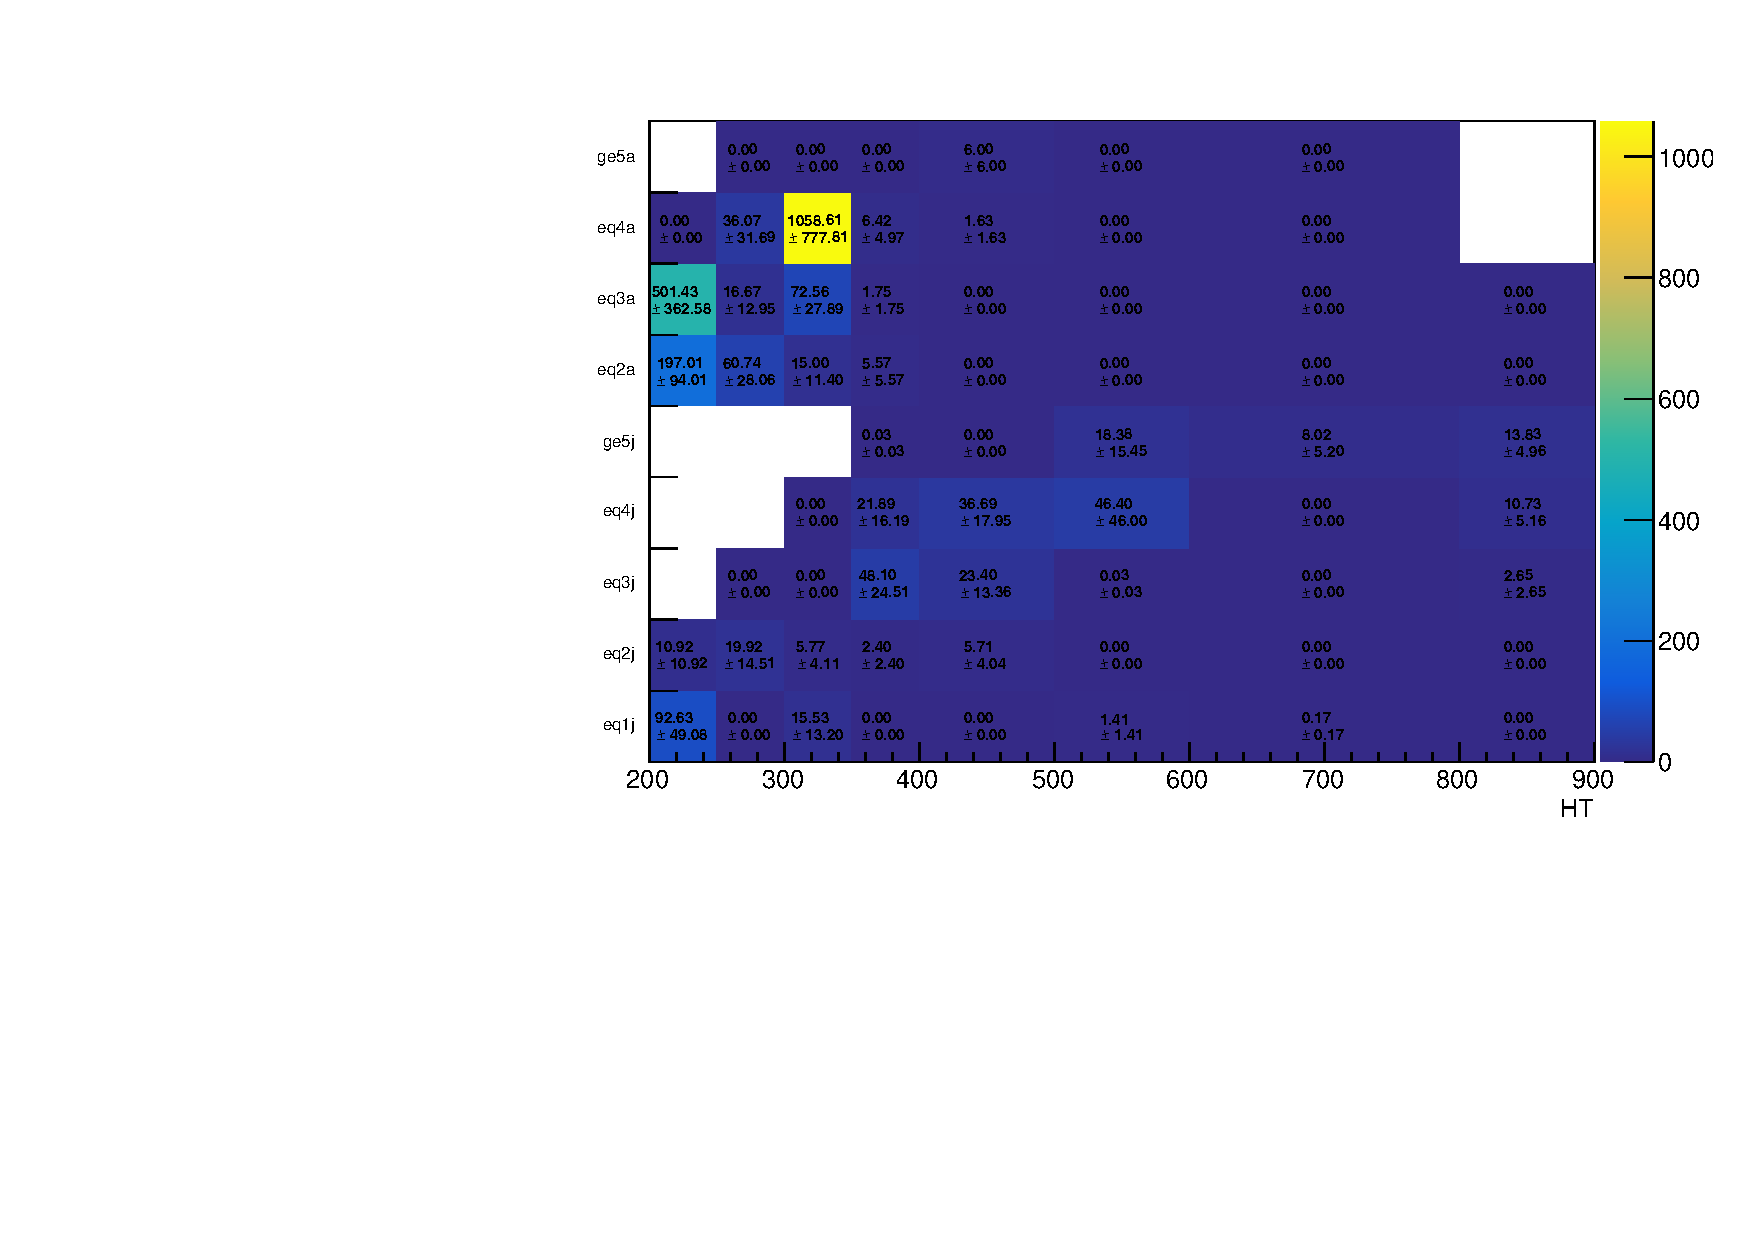
\includegraphics[width=0.4\textwidth]{Figures/qcd/plots/signalQCD_MC}
  } ~
  \subfigure[Simulated QCD events in the \mhtmet hadronic control region.\label{fig:qcd_fail}]{
    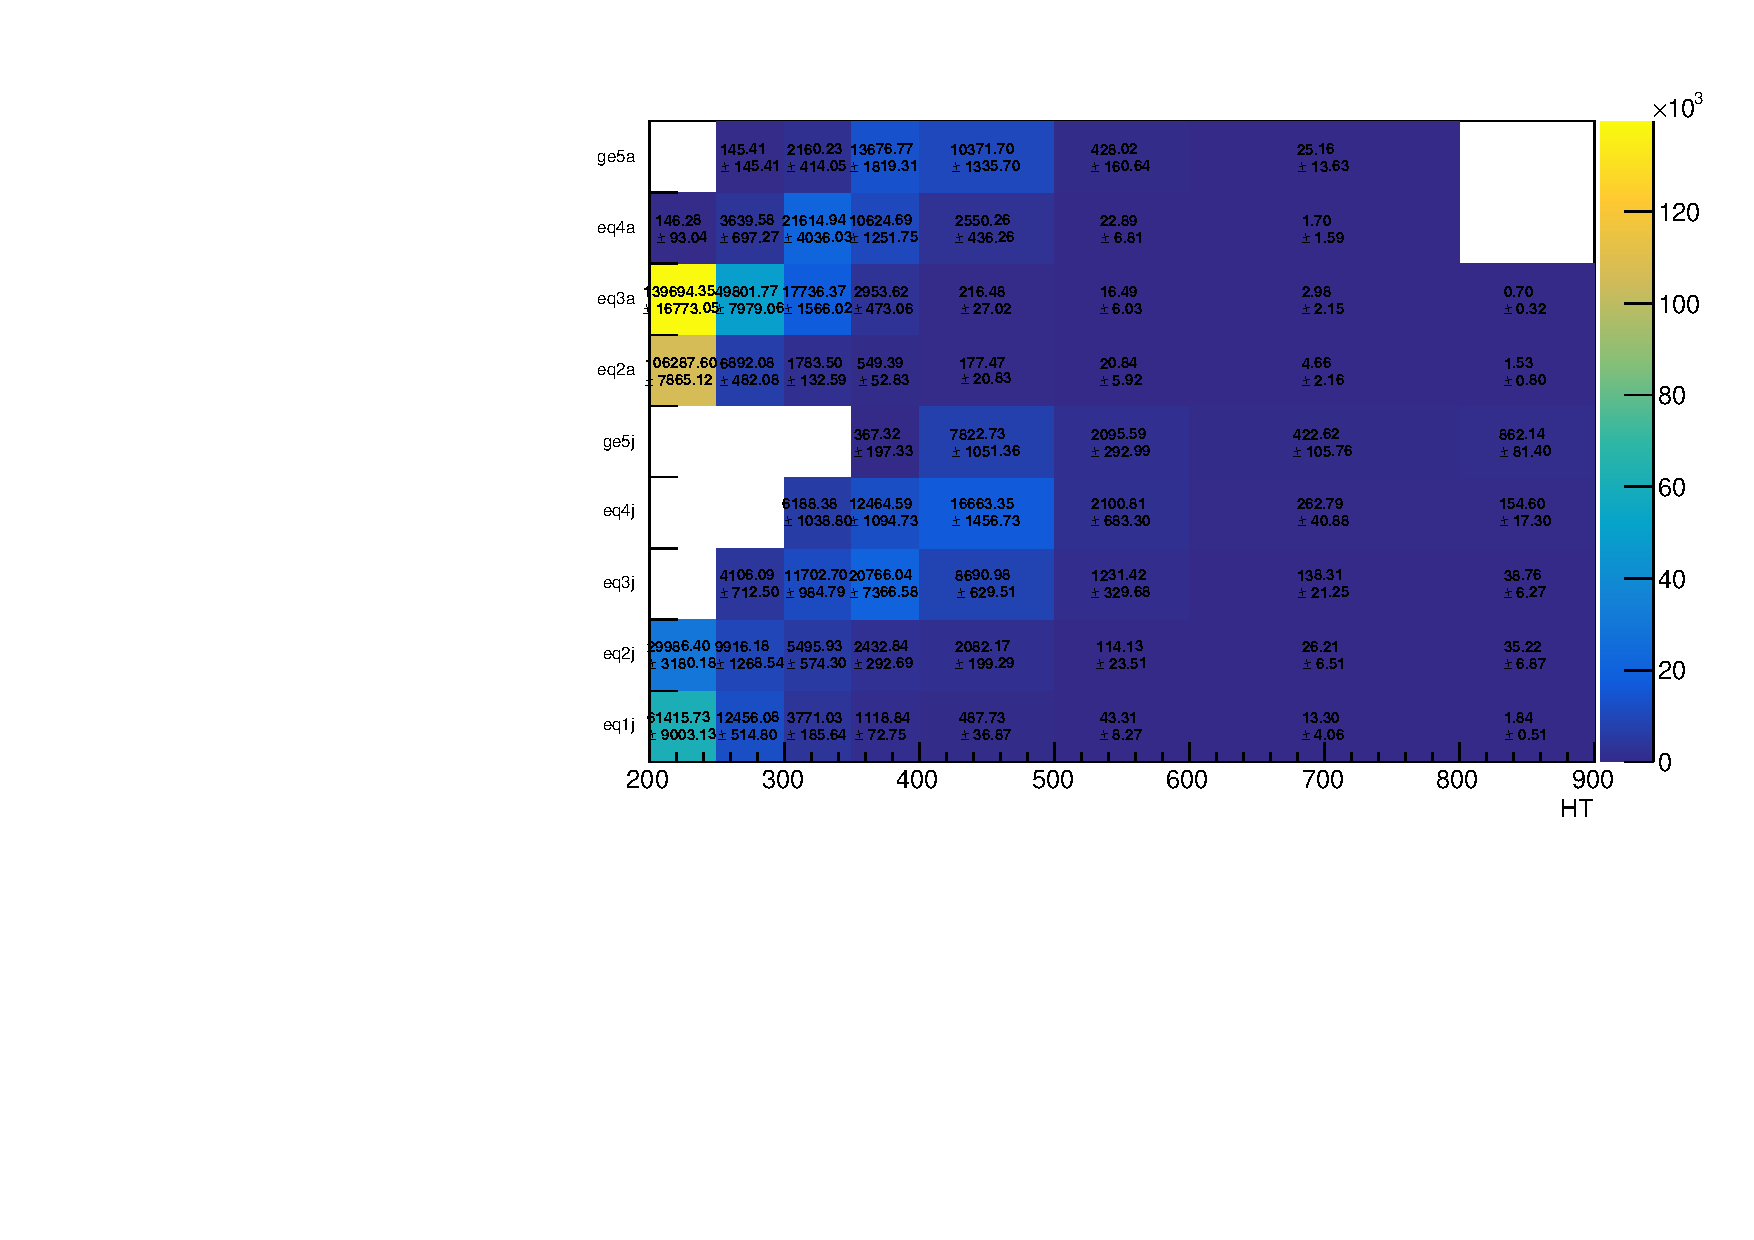
\includegraphics[width=0.4\textwidth]{Figures/qcd/plots/qcdSbQCD_MC}
  } \\
  \subfigure[Transfer factor from simulated QCD events.\label{fig:qcd_ratio}]{
    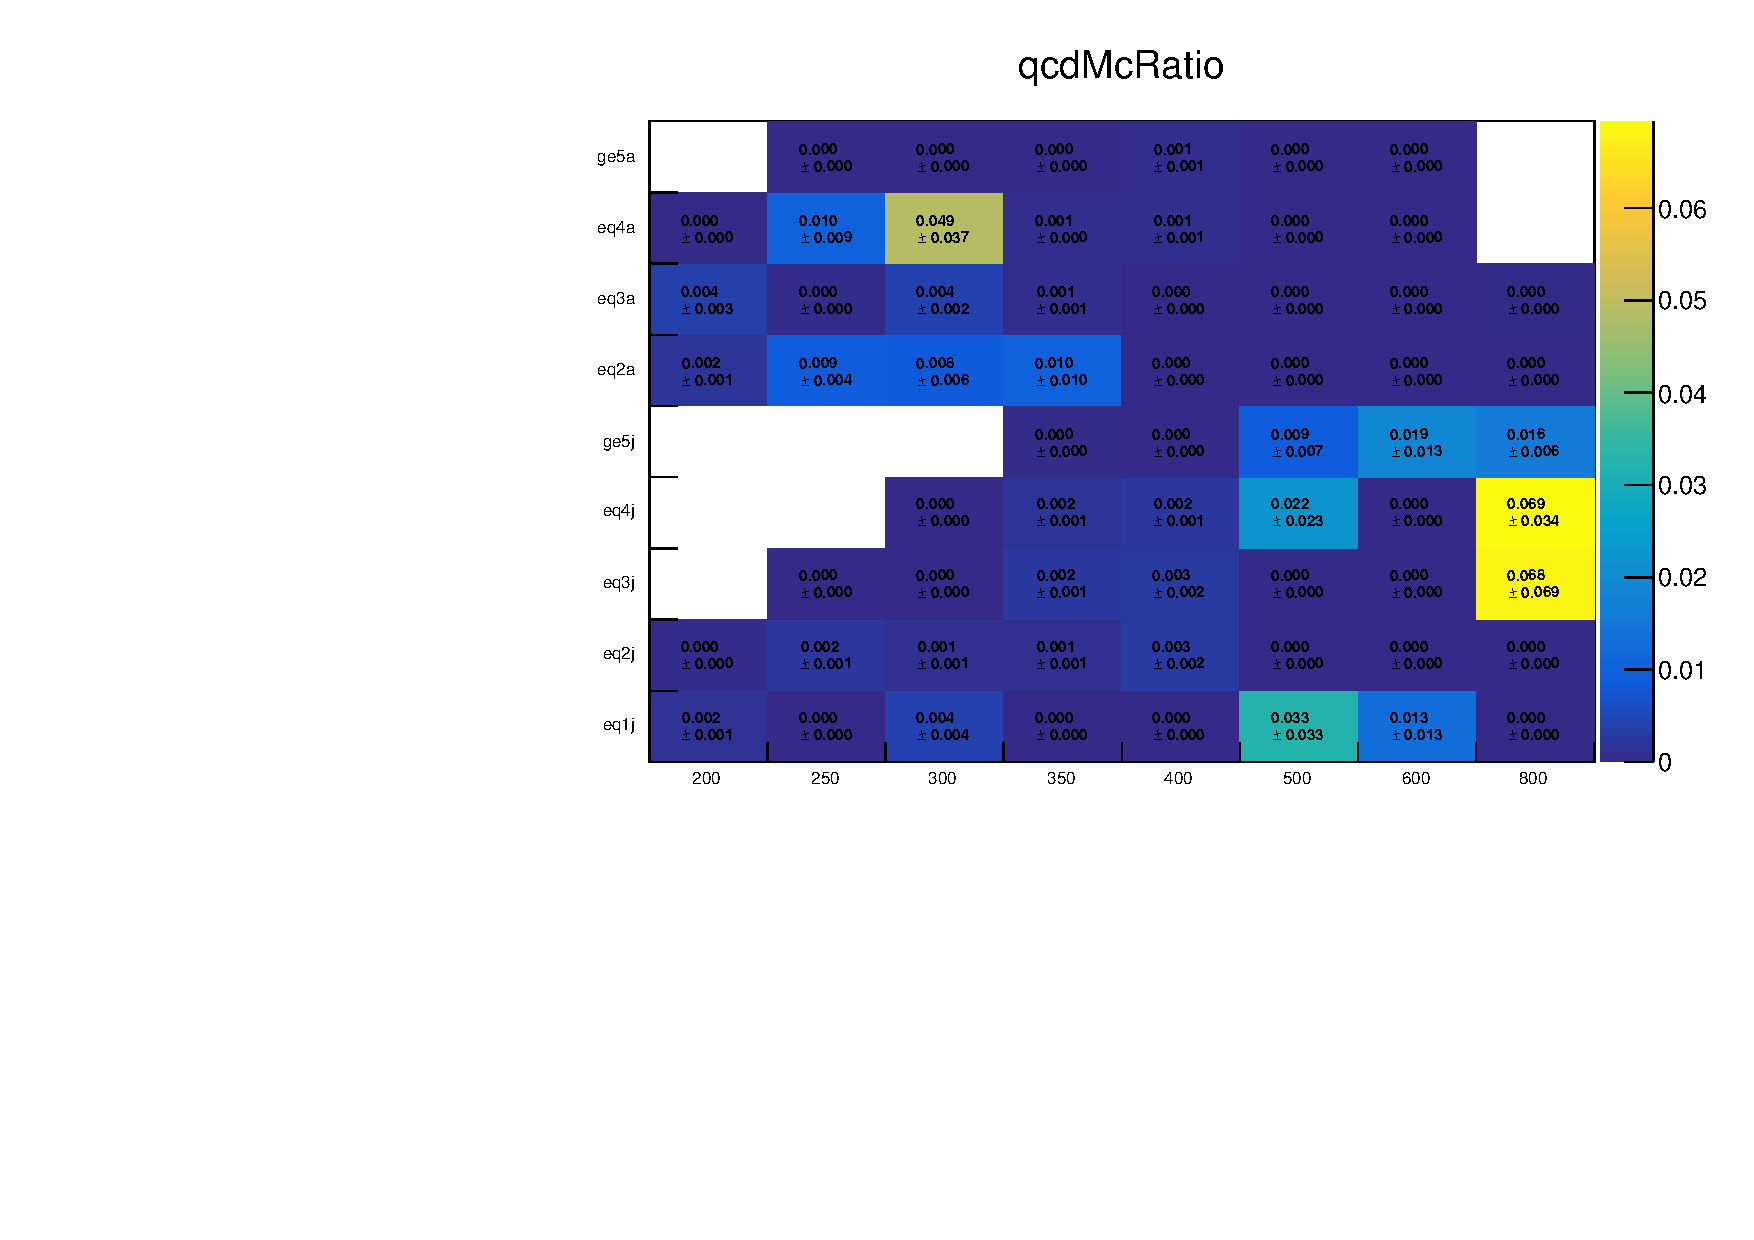
\includegraphics[width=0.4\textwidth]{Figures/qcd/plots/signalQcdDivSbQcd_MC}
  } ~ 
  \subfigure[Simulated electroweak events in \mhtmet hadronic control region.\label{fig:ewk_fail}]{
    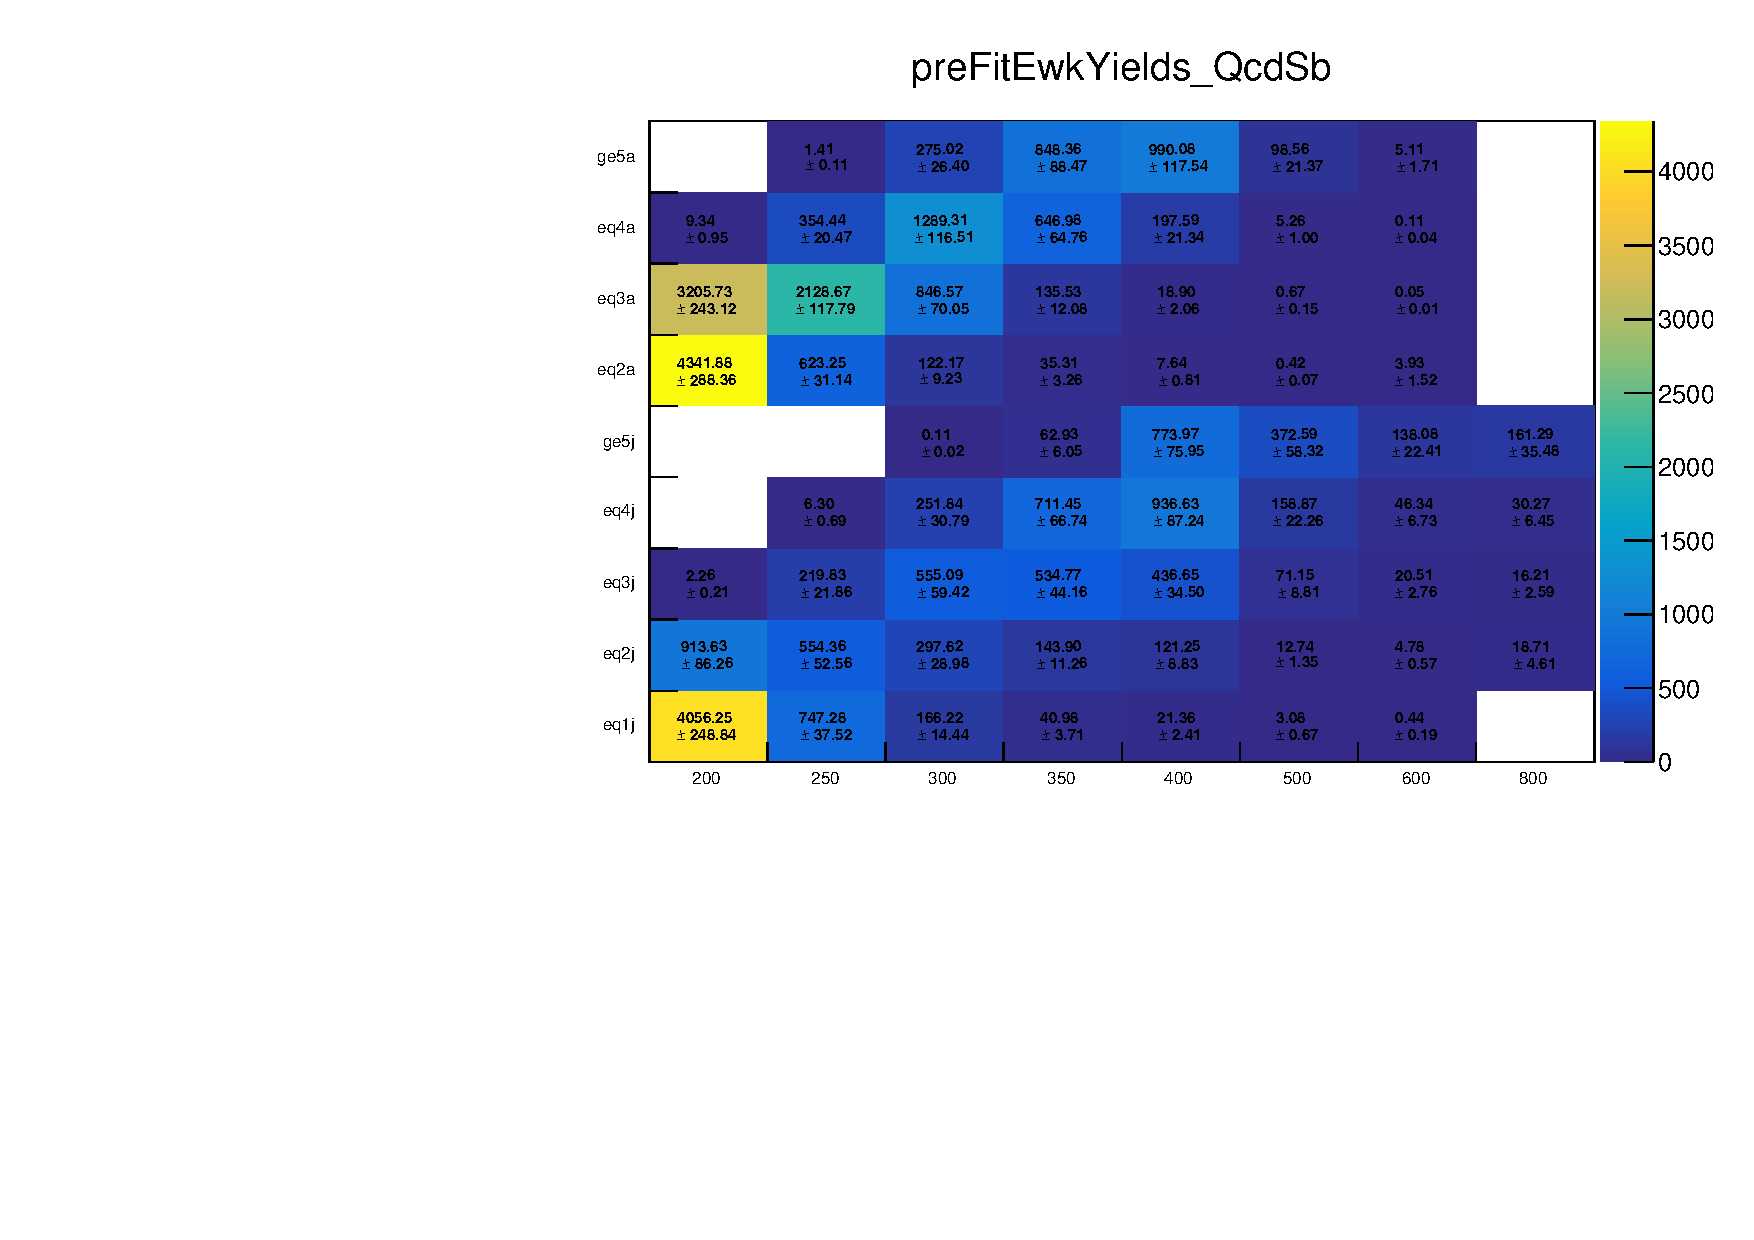
\includegraphics[width=0.4\textwidth]{Figures/qcd/plots/qcdSbEwk_MC}
   %    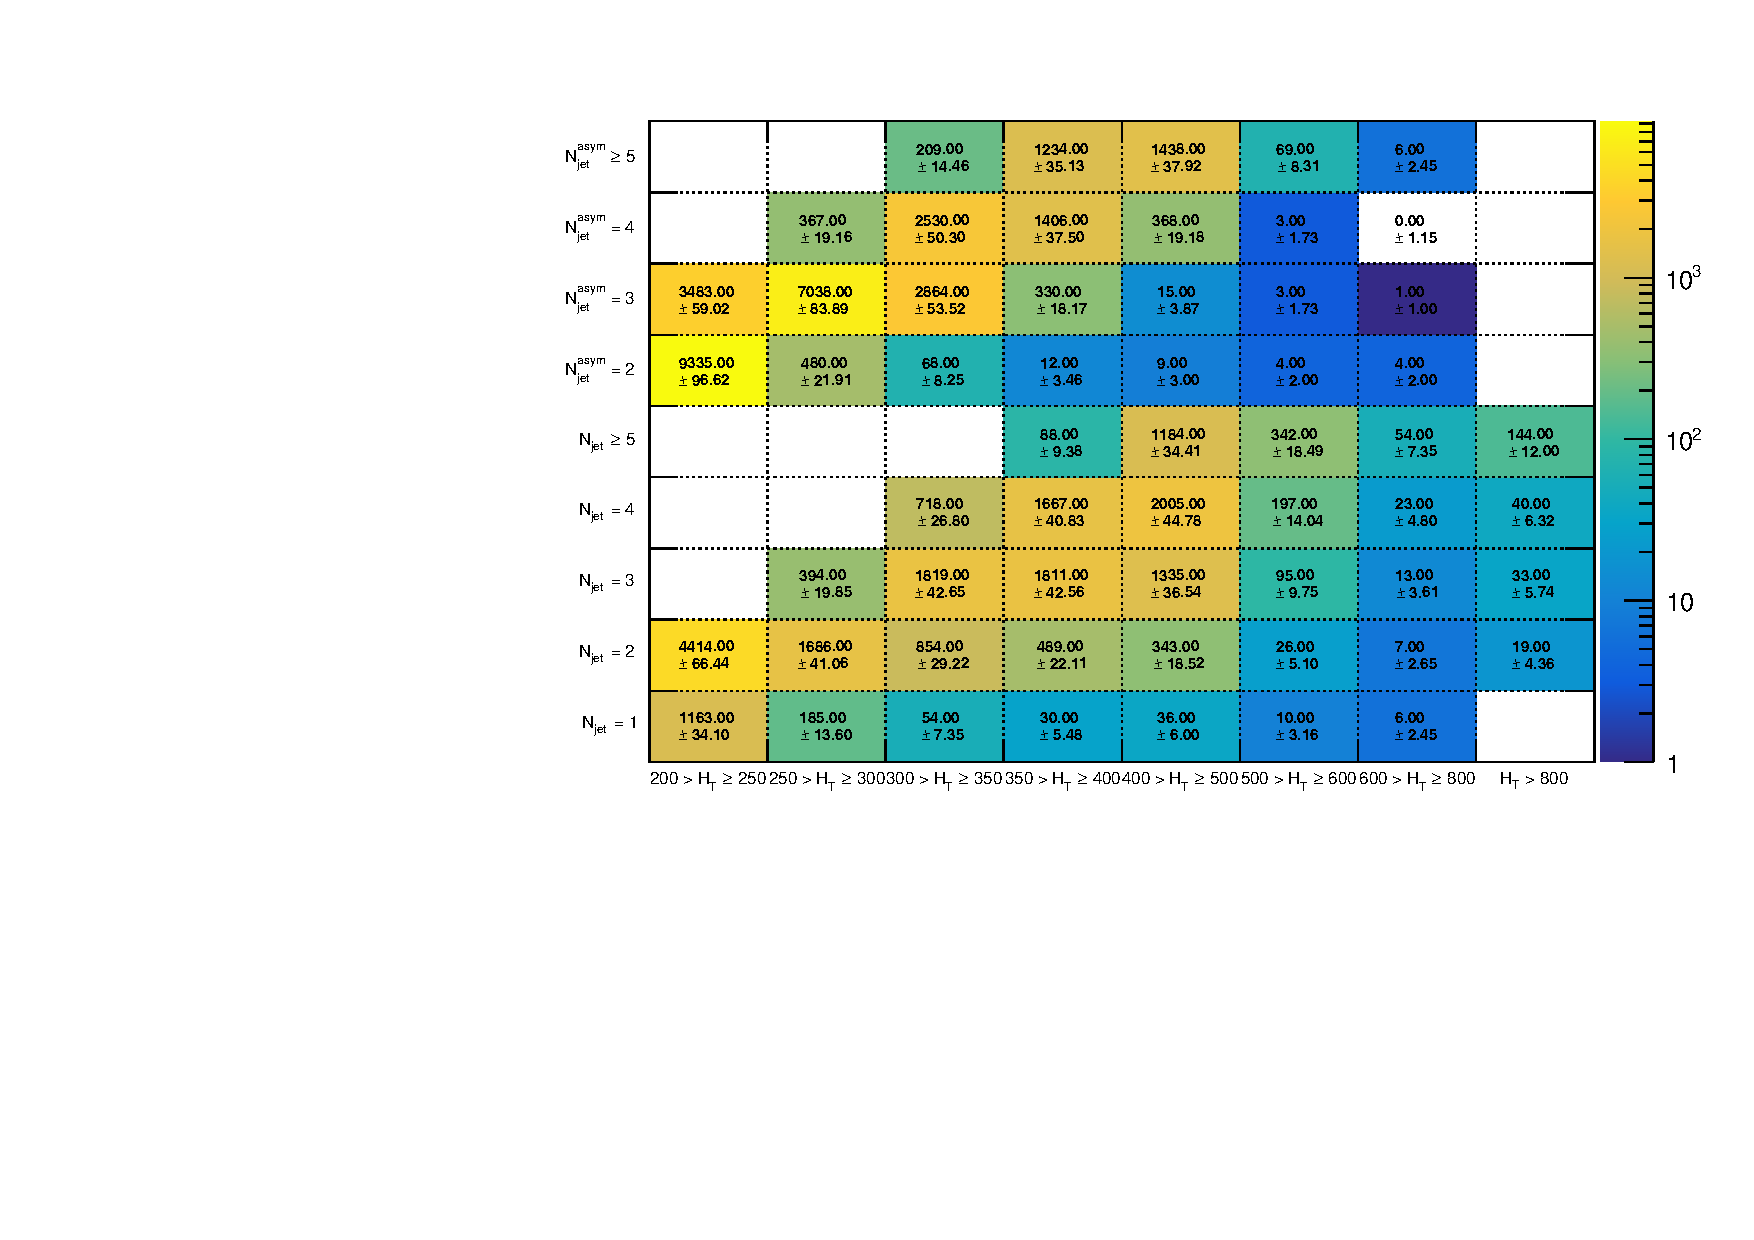
\includegraphics[width=0.4\textwidth]{Figures/qcd/v6/Ewk/SigTrig_FailMoM_NJet_vs_HT_bDPhigt0p5_Log}
  } \\
  \caption{Expected number of QCD multijet events determined from
    simulation, binned according to \njet and \scalht, that (a) satisfy
    and (b) fail the requirement $\mhtmet < 1.25$. Also shown in (c)
    is the transfer factor for QCD multijets from hadronic control to signal region, 
    again determined from simulation. Finally, (d) shows the expected number of EWK events
    (V+jets and \ttbar, plus other residual non-multijet backgrounds)
    that fail the $\mhtmet < 1.25$ requirement, again determined from
    simulation and binned according to \njet and \scalht.}
  \label{fig:qcd_plots}
\end{figure}

To detrmine the electroweak predictions in the hadronic control region transfer factors 
from the \mhtmet electroweak control regions are constructed and a simultaneous
fit is carried out, as described in Section ??. This fit includes all systematic variations discussed in Section ??, derived with
the \mhtmet~selection inverted. $N_{QCD}^{\rm control}$ is derived by including an unconstrained
contribution uncorrelated in each \njet~and \scalht~category which measures the difference between 
the electroweak prediction and the observation. The values of $N_{QCD}^{\rm control}$ are shown, 
including systematic and statistical uncertainty in Figure~\ref{fig:data_corr}. 

The signal region prediction is then made by multiplying the QCD multijet component in the hadronic 
control region by the transfer factors shown in Figure~\ref{fig:qcd_ratio}. The results of this prediction
are shown in Figure~\ref{fig:qcd_pred} with the ratio between the multijet and non-multijet background
predictions shown in Figure~\ref{fig:qcd_ewk_ratio}. The multijet component is typically $\le 1\%$. 

\begin{figure}[!h]
  \centering
  % \subfigure[Binned data counts in \mhtmet sideband.\label{fig:data_fail}]{
  %   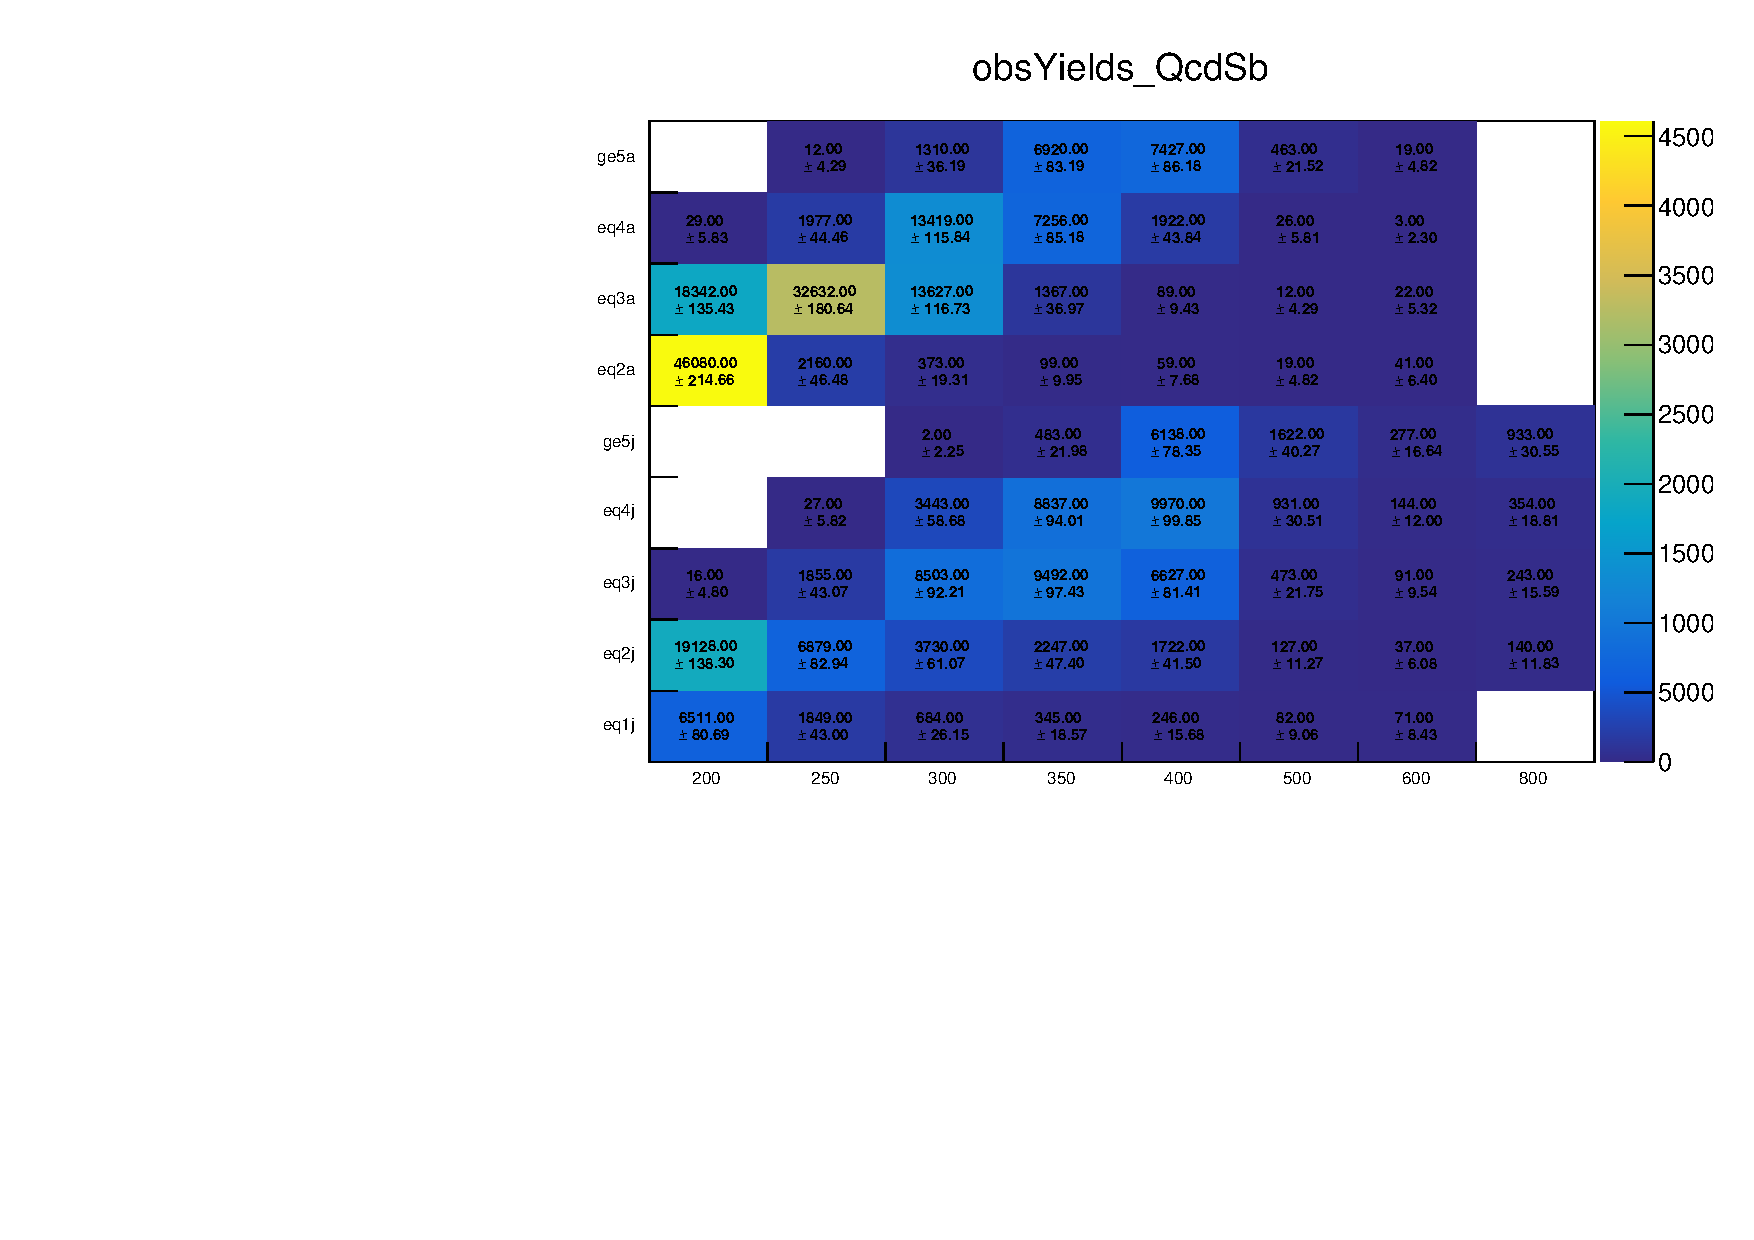
\includegraphics[width=0.4\textwidth]{Figures/qcd/plots/obsYields_QcdSb}
  % } 
  \subfigure[Predicted QCD counts in \mhtmet hadronic control region.\label{fig:data_corr}]{
    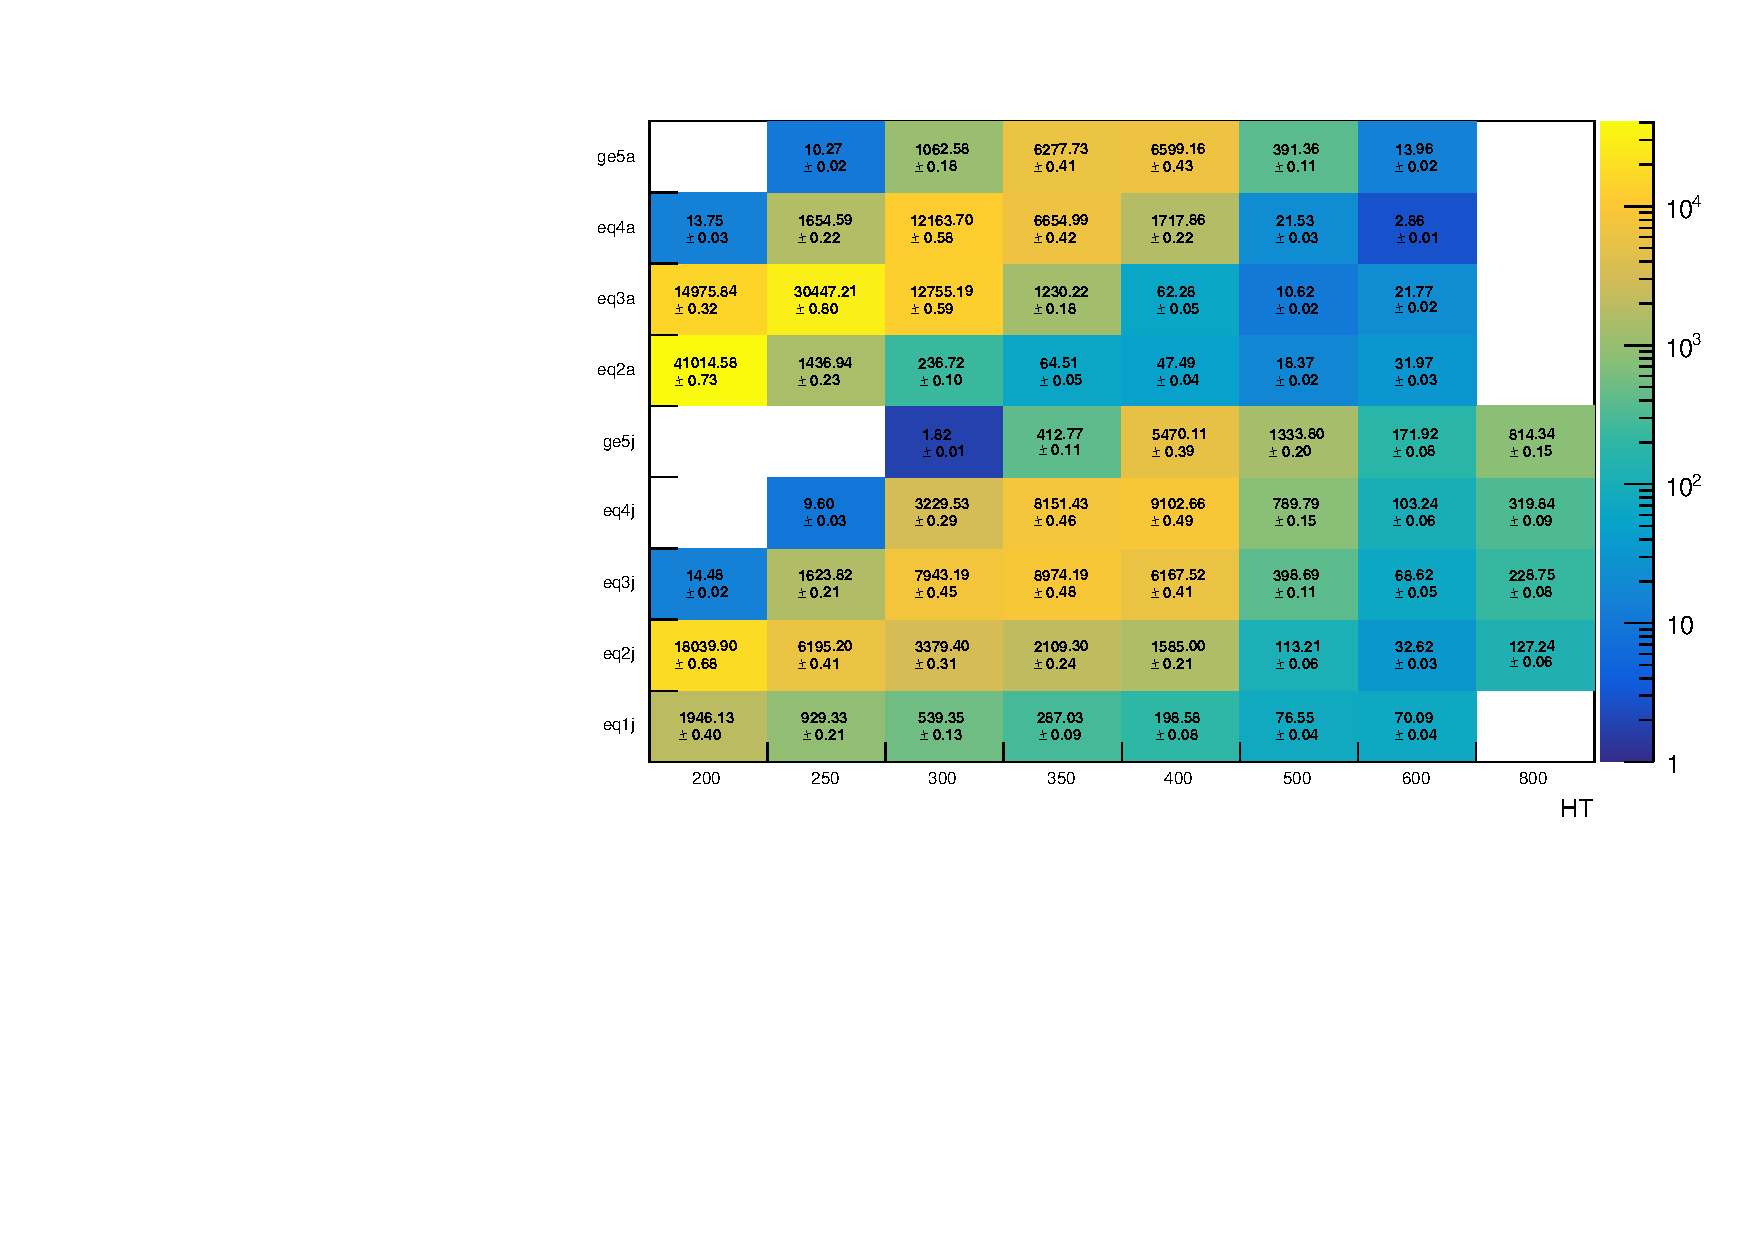
\includegraphics[width=0.4\textwidth]{Figures/qcd/plots/postFitQcdYields_QcdSb}
  } ~
  \subfigure[QCD multijet predictions in the signal region.\label{fig:qcd_pred}]{
    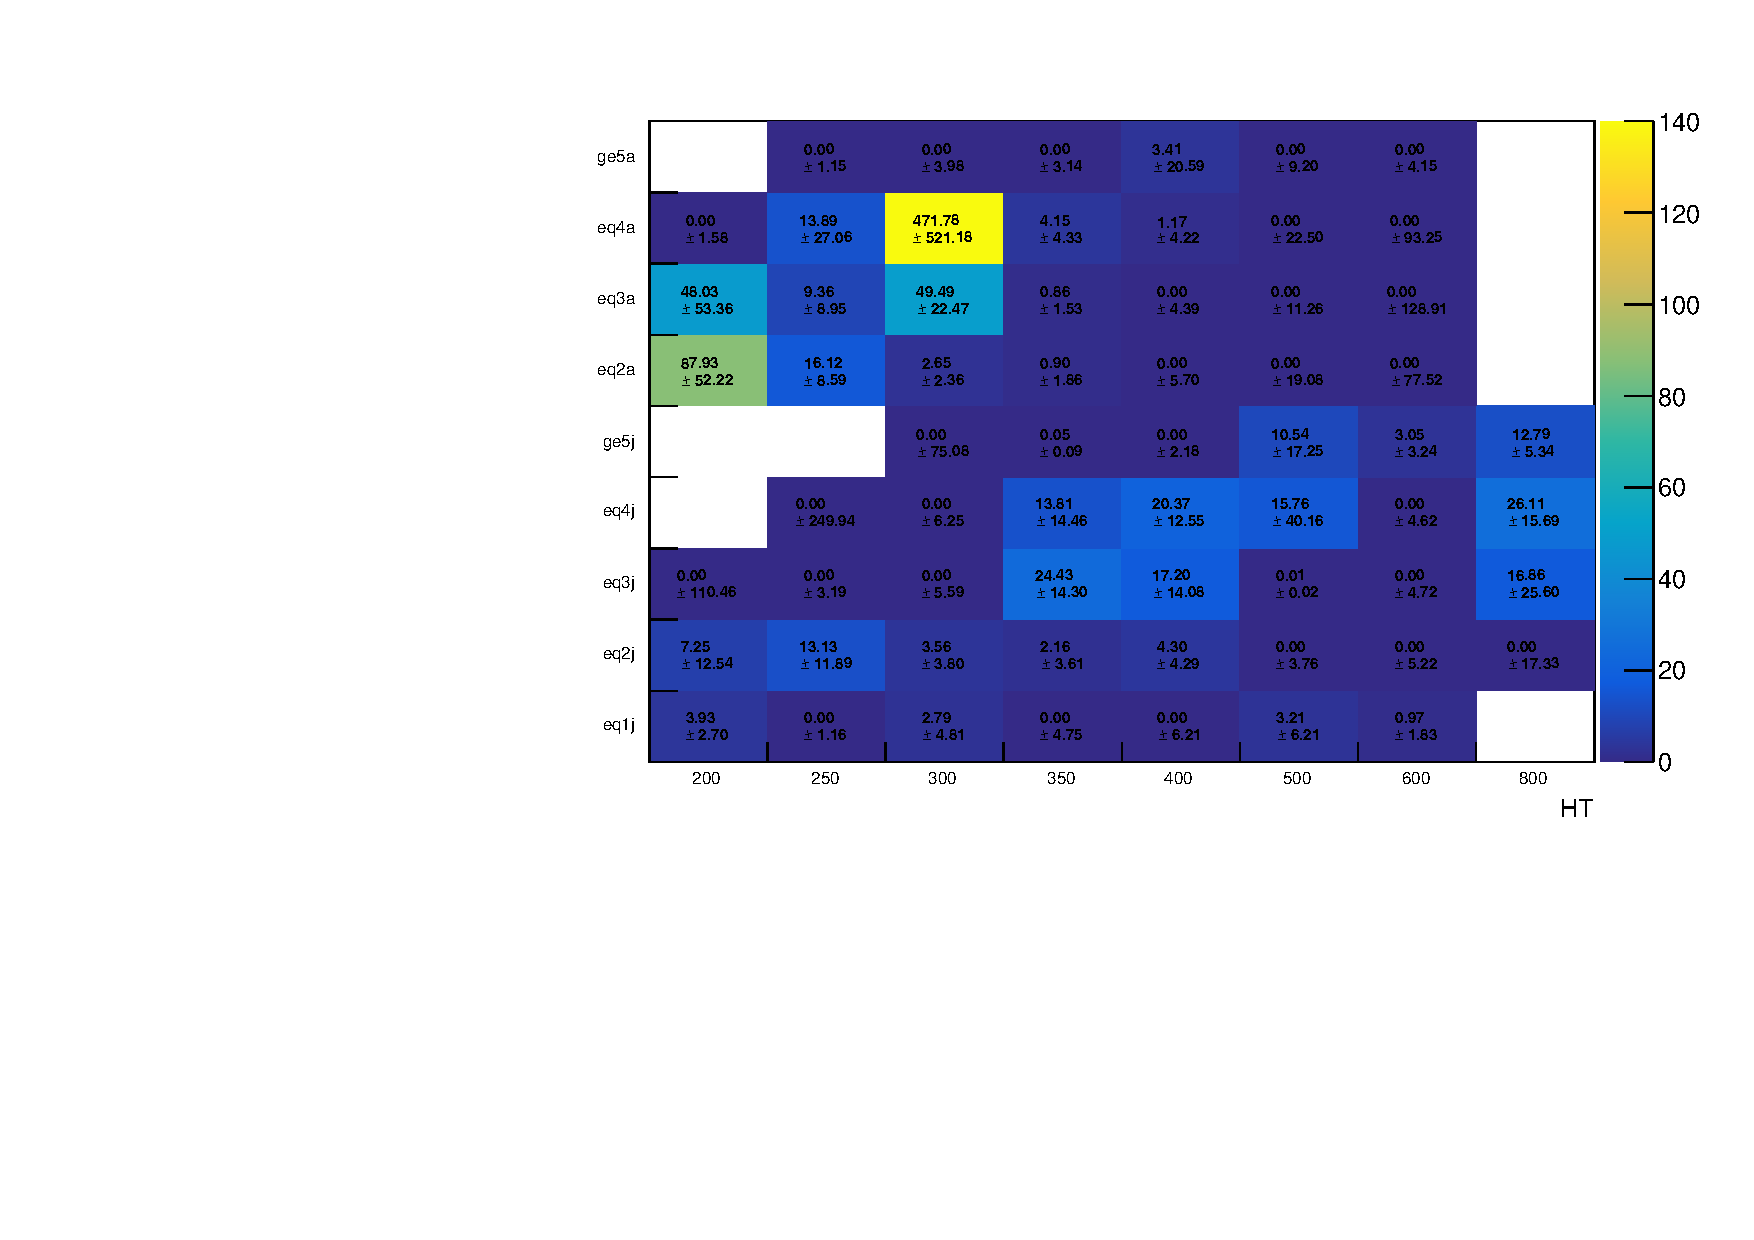
\includegraphics[width=0.4\textwidth]{Figures/qcd/plots/predictedQcdYields_Signal}
  } \\
  \subfigure[Ratio of predicted multijet and non-multijet yields.\label{fig:qcd_ewk_ratio}]{
    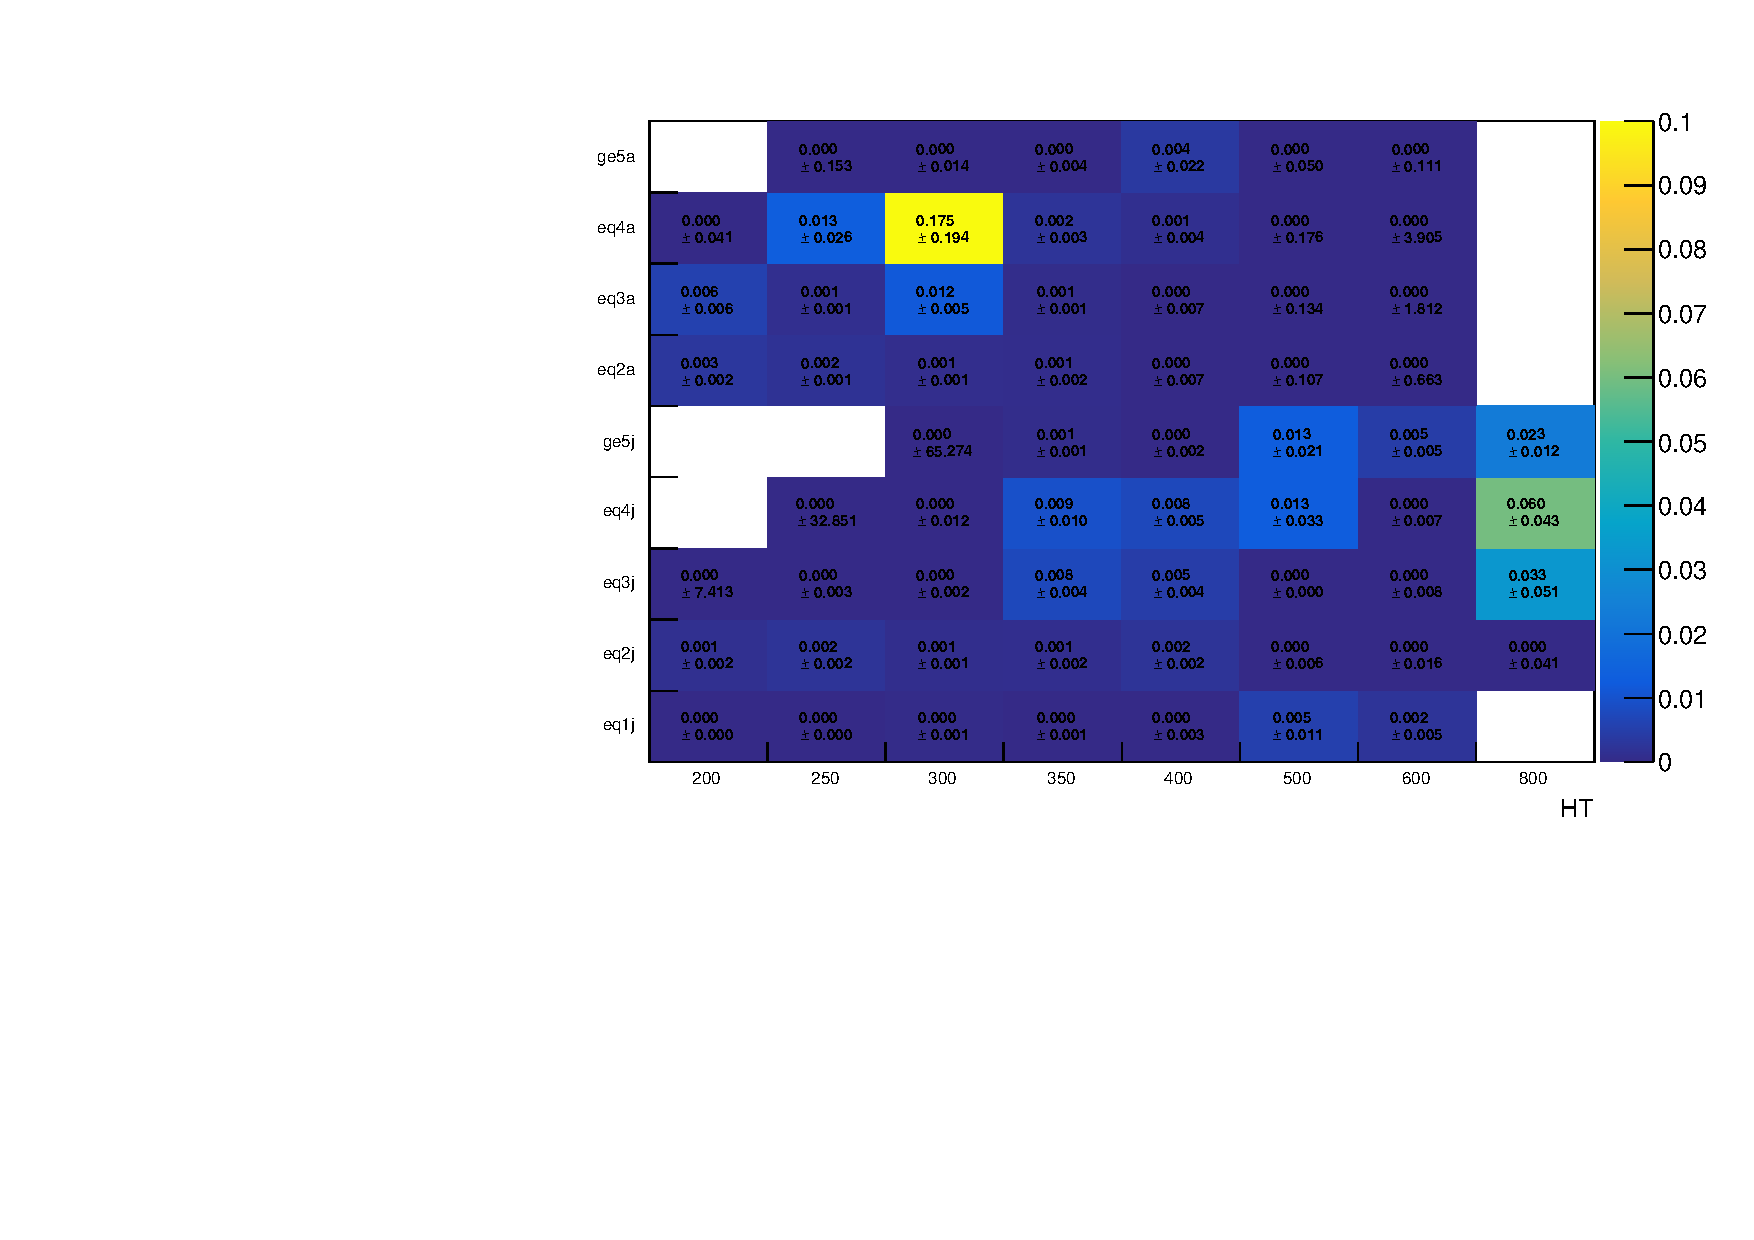
\includegraphics[width=0.4\textwidth]{Figures/qcd/plots/predictedQcdDivEwk_Signal}
  } \\
  \caption{
    The QCD yields taken from the simultaneous fit binned according to \njet and \scalht are shown in (a).
    Shown in (b) is the result of multiplying the observed multijet events predicted
    in (a) by the translation factor from the sideband to the signal
    region determined with simulation (shown in
    Fig.~\ref{fig:qcd_plots}). This gives a data driven expectation of
    the quantity of multijet background events in the signal region. 
    Finally, (c), shows the ratio of expected
    multijet background events in the signal region divided by
    non-multijet backgrounds. The multijet background is therefore
    shown to be at the percent level.}
  \label{fig:qcd_plots2}
\end{figure}

The distribution of the QCD multijet contribution in \nb~and \mht~in each \scalht~and \njet~category
is predicted using the distribution of the electroweak background. The validation 
for this approximation is discussed in Appendix ??.

\subsubsection{Validation of the multijet prediction}

The QCD multijet prediction relies on an extrapolation in the \mhtmet requirement.
Significant mismodelling of this variable can bias the QCD prediction and therefore a validation
of this extrapolation is carried out in data. This is carried out using an additional hadronic control 
region defined by inverting the $\bdphi > 0.5$ requirement. The ratio of events passing and failing 
the requirement $\mhtmet < 1.25$ is made in data and simulation, $\mathcal{R}^{data}$ and $\mathcal{R}$,
in categories of \njet~and \scalht. The ratio of $\mathcal{R}^{data}$ to $\mathcal{R}$ is shown in
Fig ?? (excluding bins with insufficient statistics). Given the small contributions ($<\sim 1\%$)
contribution of QCD multijet events, agreement within 100\% of unity is deemed acceptible. 
Given the level of agreement, a fully correlated systematic of $100\%$ is included on
the QCD contamination. This is included in addition to the uncertainty shown in 
Figure ??, taken as uncorrelated in each category.

\section{Systematic uncertainties in the transfer factors}
\label{sec:syst-uncs}
This section describes the determination of systematic uncertainties 
in the transfer factors though both variations of simulation
and using the data driven \emph{closure tests}. 

\subsection{Variation method}
In section ?? the corrections applied to the simulated samples are summarised. For each 
simulated event the correction may apply to the weight carried by that events (such as b tag efficiency
or pileup reweighting) or to the property of objects in the event (such as the jet energy scale). 
These corrections carry uncertainties that may effect the predictions of the \alphat~analysis.
To determine their effect, for each source of uncertainty the correction is varied to their
value at $\pm$ 1 $\sigma$ and the prediction from simulation re-evaluated. These uncertainties are
propagated to the likelihood as described in section ??.The inclusion of the systematic uncertainty 
in these predictions, in particular how the modifier term morphs between alternative \emph{templates} 
for $\pm$ 1 $\sigma$ variations is described in Section ??. In this section the systematic variations
of the transfer factor for each effect is discussed. The corresponding figures referenced in
this section are in ??. The effect of these systematics on the \mht shape is discussed in Section ??

\subsubsection{Pileup reweighting}

The uncertainty on the inelastic pp cross section of $\pm5\%$ is propagated by rederiving the pileup
weights for the cross section at the $\pm1\%$ sigma values. These weights are used to derive
alternative predictions for each variation. The effect on the transfer factors is shown in ??, 
typically the uncertainty introduced by pileup reweighting is small, varying from around XX\% to YY\%.

\subsubsection{Jet energy scale}
\label{sec:tfSyst_jec}
The energies of jets used in the analysis are corrected as a function of their \pt and
$\eta$ via the procedure described in Section~\ref{}. The uncertainty on
this correction is propagated through the analysis. As the \scalht and jet multiplicity binning is 
mirrored in signal and control regions, the variation in the transfer factors is small.
To avoid statistical fluctuations the variation is averaged across~\nb. The relative change 
in the transfer factors is presented as a function of \scalht and jet category 
in Fig~??. The changes are typically in the range of $1-5\%$.

\subsubsection{B-tagging efficiency}

Scale factors are applied to simulation to correct for differences in the 
b-tagging efficiencies and misidentifications between simulation and data. 
Since no extrapolation is performed in the background prediction across different 
\nb multiplicities, the analysis is expected to be robust against variations in the 
b tagging efficiency. The scale factors associated with b and c jets are varied together 
(since their measurements are correlated), while those associated with light jets are varied separately.
The relative change in the transfer factors is presented as a function of \scalht and jet category 
in Fig ~. They are typically in the range of $1-3\%$.

\subsubsection{Lepton trigger/identification/isolation efficiency}
\label{sec:tfSyst_lepton}

Leptons out of \pt and $\eta$ acceptance, or within detector
acceptance but not identified properly by lepton identification or isolation
requirements contribute to the lost lepton background. The variation 
in the lost lepton background is measured using a simulated sample with no lepton veto.
Using this sample, the variation in probability for reconstructing a lepton in the signal region,
and the variation for reconstructing a muon for the \mj control region is determined with 
appropriate correlation. Each source of systematic uncertainty 
on the muon and electron scale factors (trigger, identification and isolation) is varied seperately. 
An additional uncertainty is considered on the \mj control region for the muon tracking
scale factor. The size of the uncertainty for these variations on the transfer factors is 
shown in Fig ??.

\subsubsection{Photon trigger uncertainty}
\label{sec:tfSyst_pho}
The photon trigger correction is derived for the \gj control region. The systematic uncertainty is
taken as the size of the inefficiency measured. The relative change in the \gj transfer factor 
is presented in Fig.~\ref{fig:tfSyst_photonTrigger_gjToZinv} and is typically under $\sim3\%$.

\subsubsection{Signal trigger uncertainty}
\label{sec:tfSyst_trigger}

A systematic is taken as the difference in the efficiency measured using muon and 
electron reference triggers. The relative change in the transfer factors is typically in the range
$1-7\%$, as presented in Figs.
~\ref{fig:tfSyst_trigger_muToZinv}-\ref{fig:tfSyst_trigger_muToTtw}, 
\subsubsection{Top \pt reweighting}

The uncertainty in the top \pt~reweighting is taken as the size of the reweighting
applied to each event.
% \subsubsection{NISR??}
% \subsubsection{NLO??}

\subsection{Closure test method}
\label{sec:closure-tests}
The variations described above cover systematic uncertainties that can be modelled
in simulation. In addition, the \alphat~analysis uses the data driven control samples to
further probe sources of bias in the transfer factors due to limitations in the simulation.
The events of one control sample, B, are predicted using events from another control sample, A,
using a transfer factor from the ratio in simulation, 

\begin{equation}
N^{B}_{\text{pred}} = N^{B}_{\text{sim}}/N^{A}_{\text{sim}} \times N^{A}_{\text{data}} = TF_{\text{AB}} \times N^{A}_{\text{data}},
\end{equation}

the agreement between the samples is then measured by the ratio, 

\begin{equation}
R_{\text{AB}} = \frac{N^{A}_{\text{data}}-N^{B}_{\text{pred}}}{N^{B}_{\text{pred}}}.
\end{equation}


The closure between the samples is defined as the signficance of the deviation of this ratio from zero 
considering statistical uncertainties in both observation and simulation in samples A and B.
The tests are performed seperately per \njet and \scalht category to investigate the level of closure. 
The uncertainties are derived per \scalht bin by merging the \njet categories into 
the symmetric and asymmetric (including monojet) topologies. For each such category, the systematic
uncertainty is defined by the value of $R_{\text{AB}}$ added in quadrature to its statistical uncertainty.
For tests involving the \mmj sample, which has lower statistical power, pairs of \scalht bins 
are merged for the closure tests. 

The systematics derived using these tests are applied to the transfer factors. They are considered
as un-correlated per \scalht and jet topology (correlated in other categorisations). The tests carried 
out and systematic biases probed are discussed below.

\subsubsection{Extrapolation in \alphat and \bdphi}

The control regions do not select on the dedicated variables \alphat and \bdphi. The
bias this may introduce due to potential modelling differences in data and simulation is
probed with tests in data. To test the \alphat (\bdphi) modelling the \mj sample is divided 
into events with an \alphat (\bdphi) requirement and with the requirement inverted (corresponding
to samples A and B in equation ??). This requirement is decided by the signal \scalht bin for 
\alphat and is 0.5 for \bdphi. The systematic is derived from the \alphat closure tests for
bins with $\scalht < 900 \GeV$ and the \bdphi tests for $\scalht > 900 \GeV$.

The results of these tests are shown in figure ?? (AWAITING DECISION FOR HOW THESE SYSTS WILL BE DERIVED)

\subsubsection{Modelling of the W acceptance due to polarisation effects}

The production mechanism of W bosons from pp collisions means high \pt W bosons are predominantly left 
handed~\cite{lhW}. This means that $W^{+}$ bosons will decay to the left handed neutrino \emph{along}
its direction of motion while the lepton points backwards. The $W^{-}$ bosons behave oppositely, decaying
to the lepton along its direction of motion. As the signal region relies on boosted neutrinos 
for acceptance and the \mj control region on a boosted lepton there is a corresponding preponderance
of $W^{+}$ over $W^{-}$ in the signal region compared to \mj control region. This may introduce bias
in the prediction and a data driven test is carried out by splitting the \mj sample into events 
with either a $\mu^{+}$ or $\mu^{-}$ (corresponding to samples A and B in equation ??).

The results of these tests are shown in figure ?? (AWAITING DECISION FOR HOW THESE SYSTS WILL BE DERIVED)

\subsubsection{Modelling of the W/Z ratio}

The \alphat analysis uses \mj events to predict the \znunu background. The extrapolation 
between W and Z is tested by using the \mj control region to predict the \mmj control region.
These tests probe differences in the modelling of the Z and W, potential acceptance and
reconstruction effects (expected to be subdominant) and the effect of 
the \ttbar contribution to \mj.

The results of these tests are shown in figure ?? (AWAITING DECISION FOR HOW THESE SYSTS WILL BE DERIVED)
\subsubsection{Modelling of the Z/$\gamma$ ratio}

The \alphat analysis uses \gj events to predict the \znunu background. The extrapolation 
between $\gamma$ and Z is tested by using the \gj control region to predict the \mmj control region.
These tests probe differences in the modelling of the Z and $\gamma$ as well as potential acceptance and
reconstruction effects for $\mu$ and $\gamma$. 

The results of these tests are shown in figure ?? (AWAITING DECISION FOR HOW THESE SYSTS WILL BE DERIVED)

\subsubsection{Modelling of the W/\ttbar admixture}

The \mj control region is used to predict the \wj and \ttbar processes. However, the admixture
between these processes may not be identical in the signal and control region (see Appendix ??).
To probe potential bias introduced due to this admixture change the sample is split into events with
0 and 1 b-tag (corresponding to samples A and B in equation ??). These tests will also probe 
uncertainties related to the b-tagging efficiency and related scale factors. As this uncertainty 
is explicitely considered this closure test is not used to derive systematic uncertainties.

The results of these tests are shown in figure ?? (AWAITING DECISION FOR HOW THESE SYSTS WILL BE DERIVED)

\subsection{Summary}

The size of the systematic uncertainties and the bins to which they are applied
are summarised in the table below.

\section{The \mht dimension}
\label{sec:syst-on-shape}

The estimate of the number of events per (\njet,~\nb,~\scalht) bin,
integrated over \mht, is derived from data control samples, with
the associated systematic uncertainty determined as 
described in Sec.~\ref{sec:closure-tests}. This section
describes the method used to assess the systematic uncertainties in
the distribution of events according to \mht. A data driven approach is
utilised under the hypothesis of zero bias in the data and MC agreement.
The level of closure in the control regions is used
to derive alternative templates accounting for systematic uncertainties.

When looking at the \mht dimension inclusively in \scalht there are
large theoretical uncertainties that originate from mixing events
at different scales. These uncertainties can be mitigated if the events 
are binned according to a variable, such as \scalht, 
which is strongly correlated with the scale of the event. 
After this categorisation is applied, the uncertainty in 
the distribution of the \mht variable
(as well as any other MET-like variable) is expected to be 
mainly affected by the MC modelling of the particle 
decays and, to a lesser extent, by jet reconstruction effects, 
such as jet energy scale and resolution. 
This approach, which will be often referred to as \textit{scale anchoring}
in the following, is used in this analysis. The distribution in \mht
is measured in data using the control regions and compared to MC
to determine the validity of the zero bias hypothesis after scale anchoring.

In Sec.~\ref{sec:valid13} the 13 \TeV data is used used 
to validate the scale anchoring approach. 
In Sec.~\ref{sec:systMhtDimension} 
the procedure used to extract the systematic uncertainties in the 
\mht dimension is described and results shown with 13 \TeV data. 

The systematic uncertainties extracted from the control regions
are added in addition to systematic from variations in simulation.
The variation in simulation follows the same procedure as described in
?? and a comparason of the different sources of systematic uncertainty
is presented in Section~\ref{sec:mcSystStudiesShape}.

\subsection{Validation using control regions in data}
\label{sec:valid13}
To parameterise the data/MC agreement
for the three electroweak control regions
orthogonal polynomials are used such that odd and even powers 
are decorrelated \cite{cohen2013applied}. 
The $n^{th}$ order orthogonal polynomial which is fitted to the data/MC 
distribution is defined in Eq.~\ref{equ:orthog-polynomial}.

\begin{equation}
  \label{equ:orthog-polynomial}
  f_n(x) = \sum_{k=0}^{k=n}{(p_k)\times(\bar{x}-x)^k}
\end{equation}

where $\bar{x}$ is the weighted mean of the distribution and $p_k = 0$ 
implies the $k^{th}$ order is negligible.
In Fig.~\ref{fig:linearMotiv} the data/MC 
distribution against \mht for the control region selection 
(detailed in \cite{Khachatryan:2016pxa}) is shown inclusive 
in \scalht and categories. By fitting a first order
orthogonal polynomial it can be seen that there is a large bias. 
This bias in the data/MC agreement is expected as events 
at different scales are mixed.
The first order orthogonal polynomial
is used to measure the level of bias remaining 
when the \mht dimension is binned in \scalht.
This allows the normalisation parameter to be
decorrelated from the parameter which controls
the distribution in \mht.
The normalisation in each \scalht bin and its systematics 
is then defined following the data-driven method used in Run 1, see Sec,~\ref{sec:systMhtDimension} for details.
\begin{figure}[h!]
  \centering
  \subfigure[\mj]{
    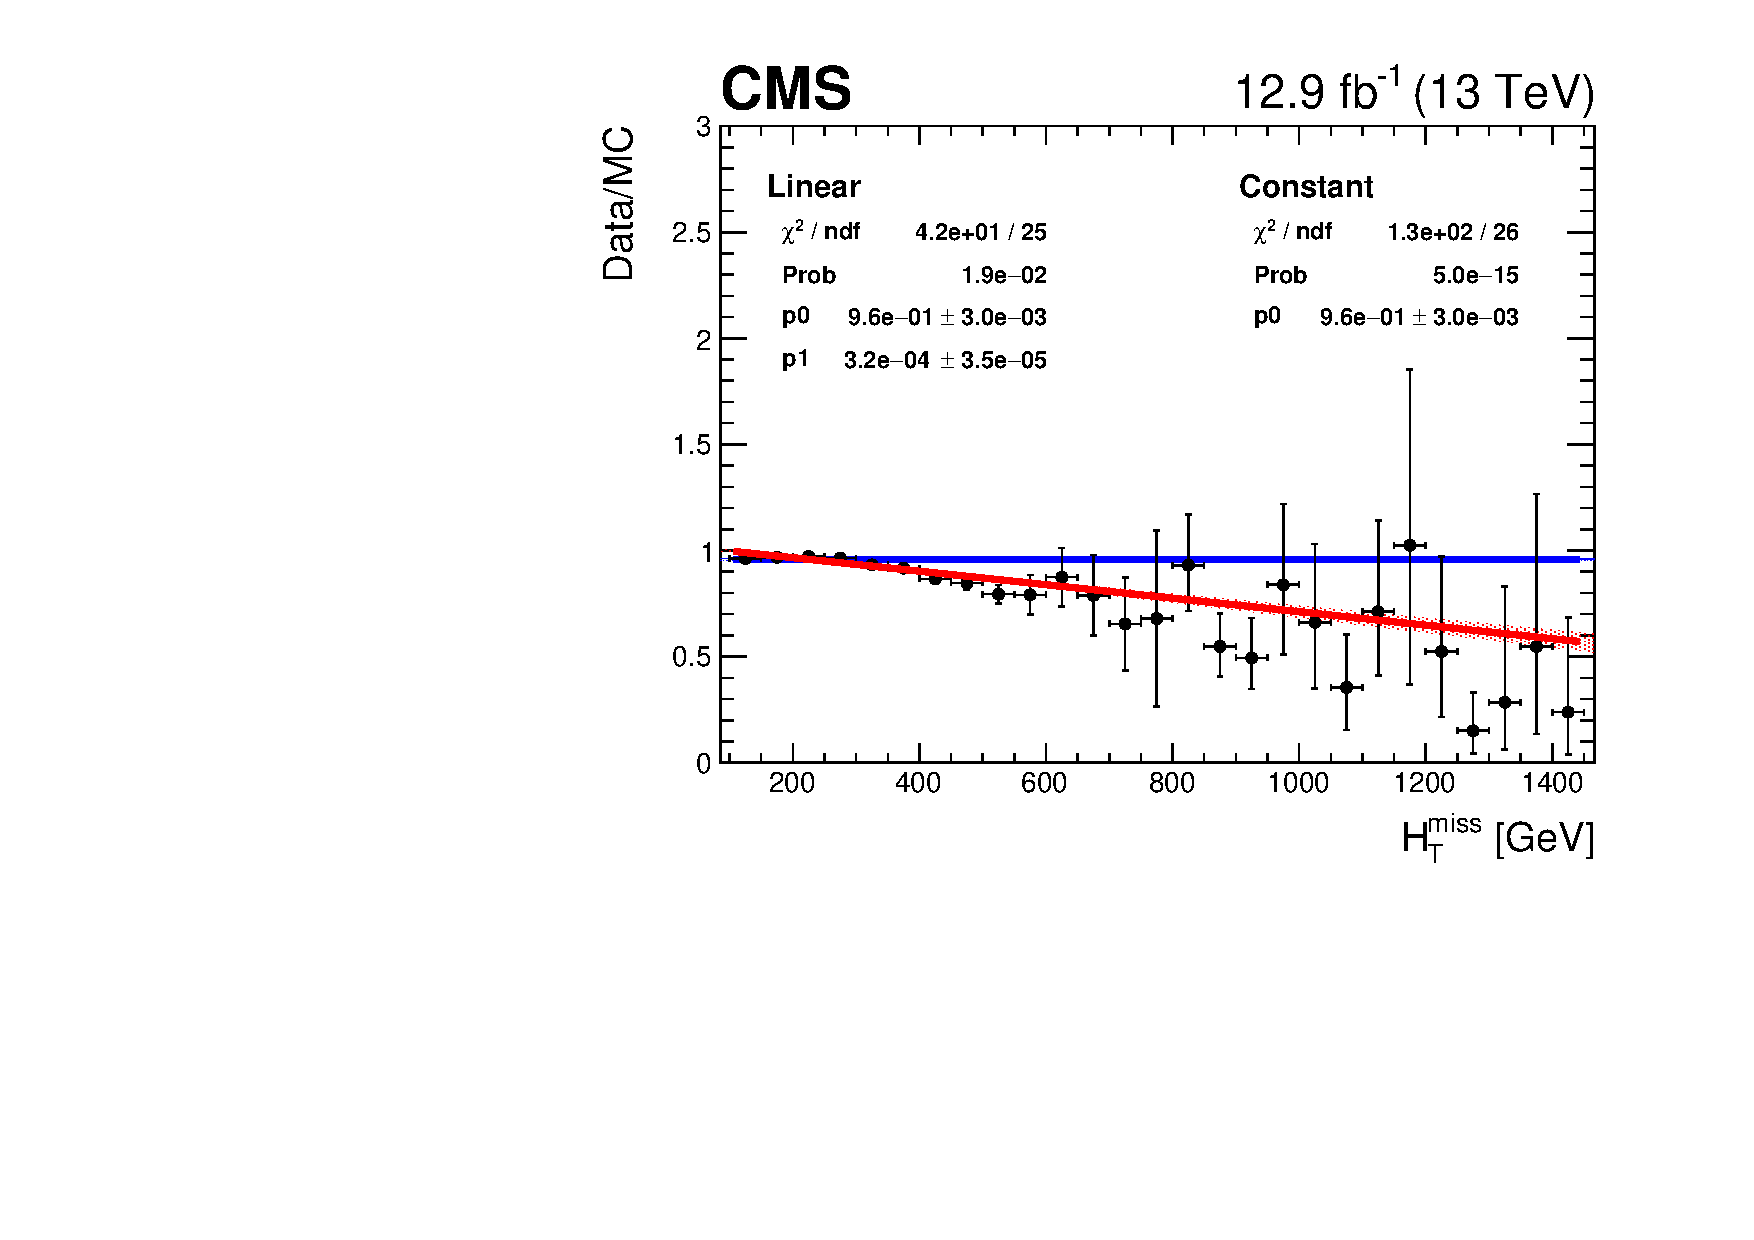
\includegraphics[width=0.5\textwidth]{Figures/backgroundPrediction/shapeOutput12FbInc/scale_ht_variable_mht/SingleMu/Inc_Inc/finalFits/mht_Inc_Inc_ht_Inc_SingleMu_Graph.pdf}
  }~~
  \subfigure[\gj]{
    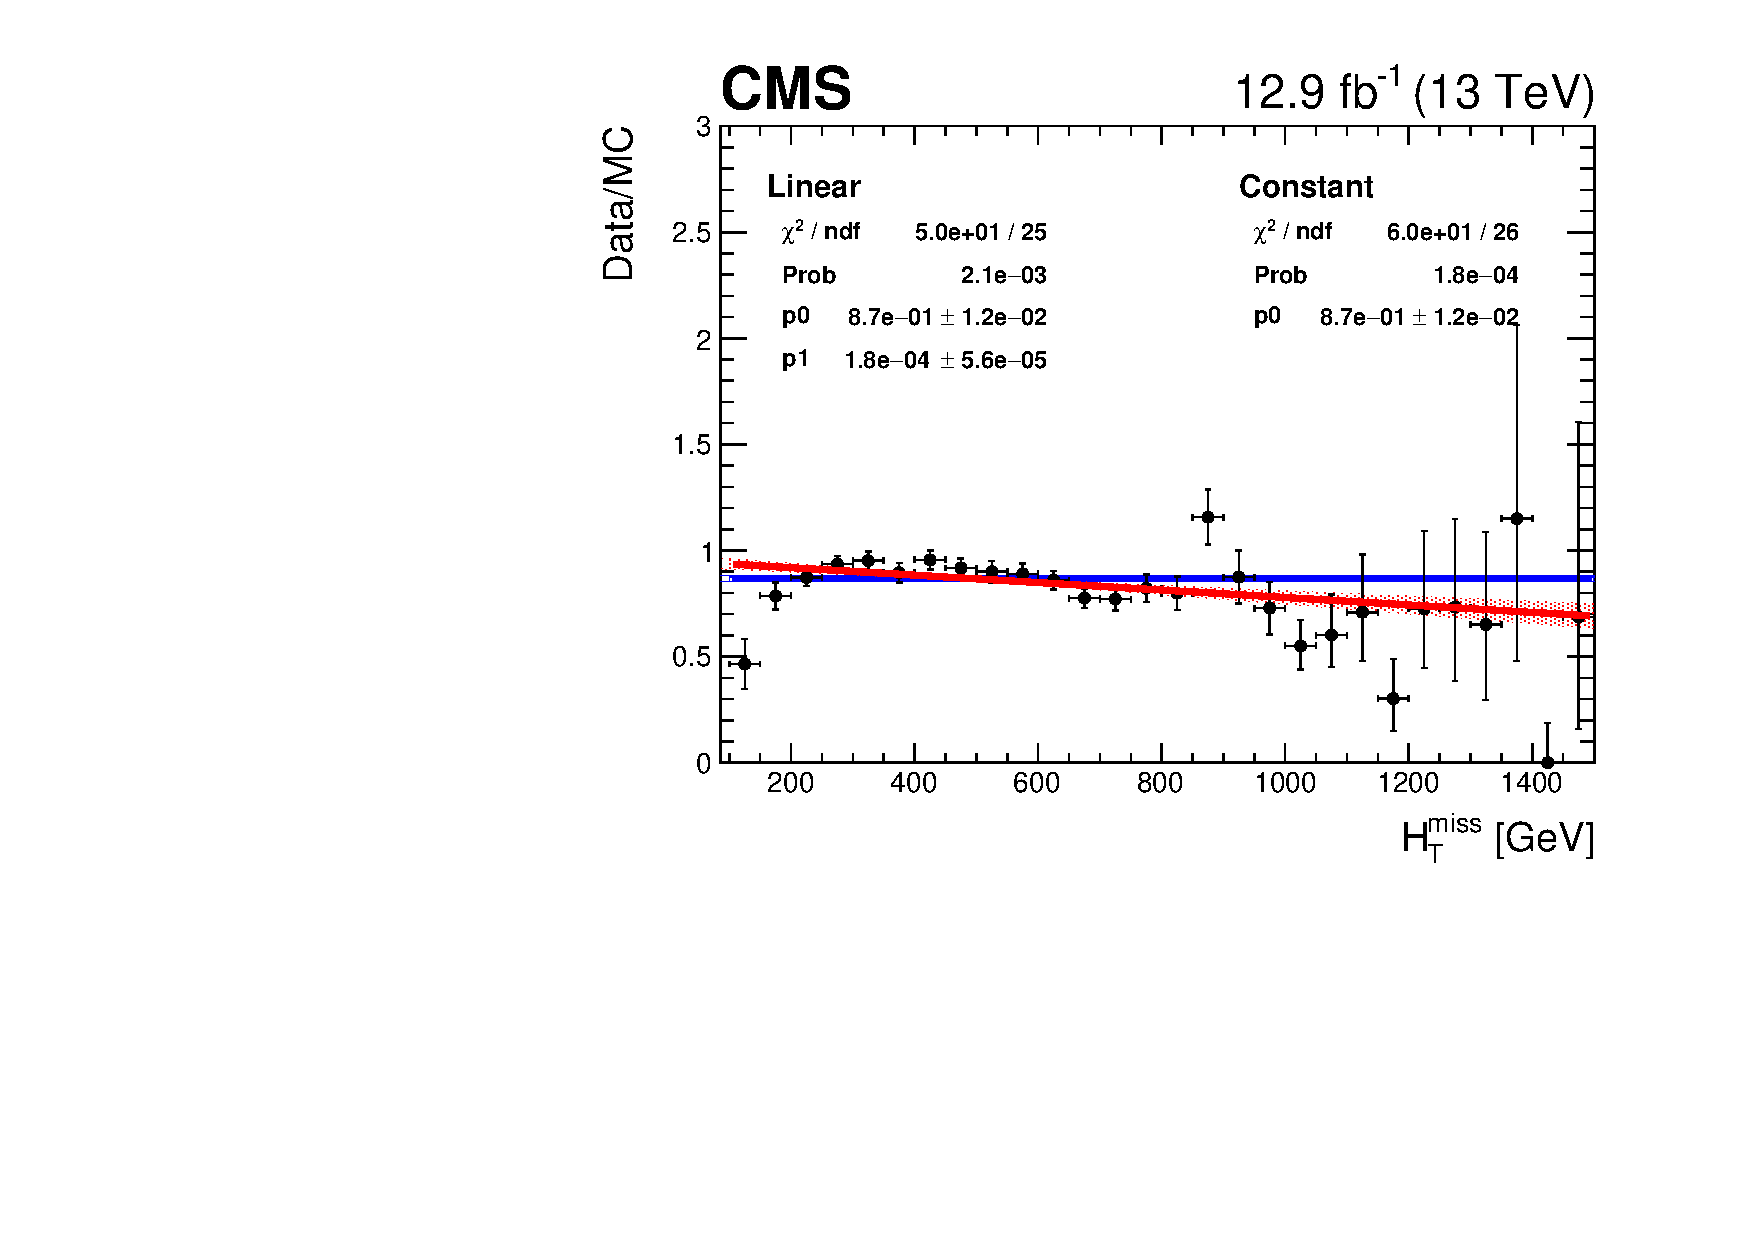
\includegraphics[width=0.5\textwidth]{Figures/backgroundPrediction/shapeOutput12FbInc/scale_ht_variable_mht/SinglePhoton/Inc_Inc/finalFits/mht_Inc_Inc_ht_Inc_SinglePhoton_Graph.pdf}
  }\\
  \subfigure[\mmj]{
    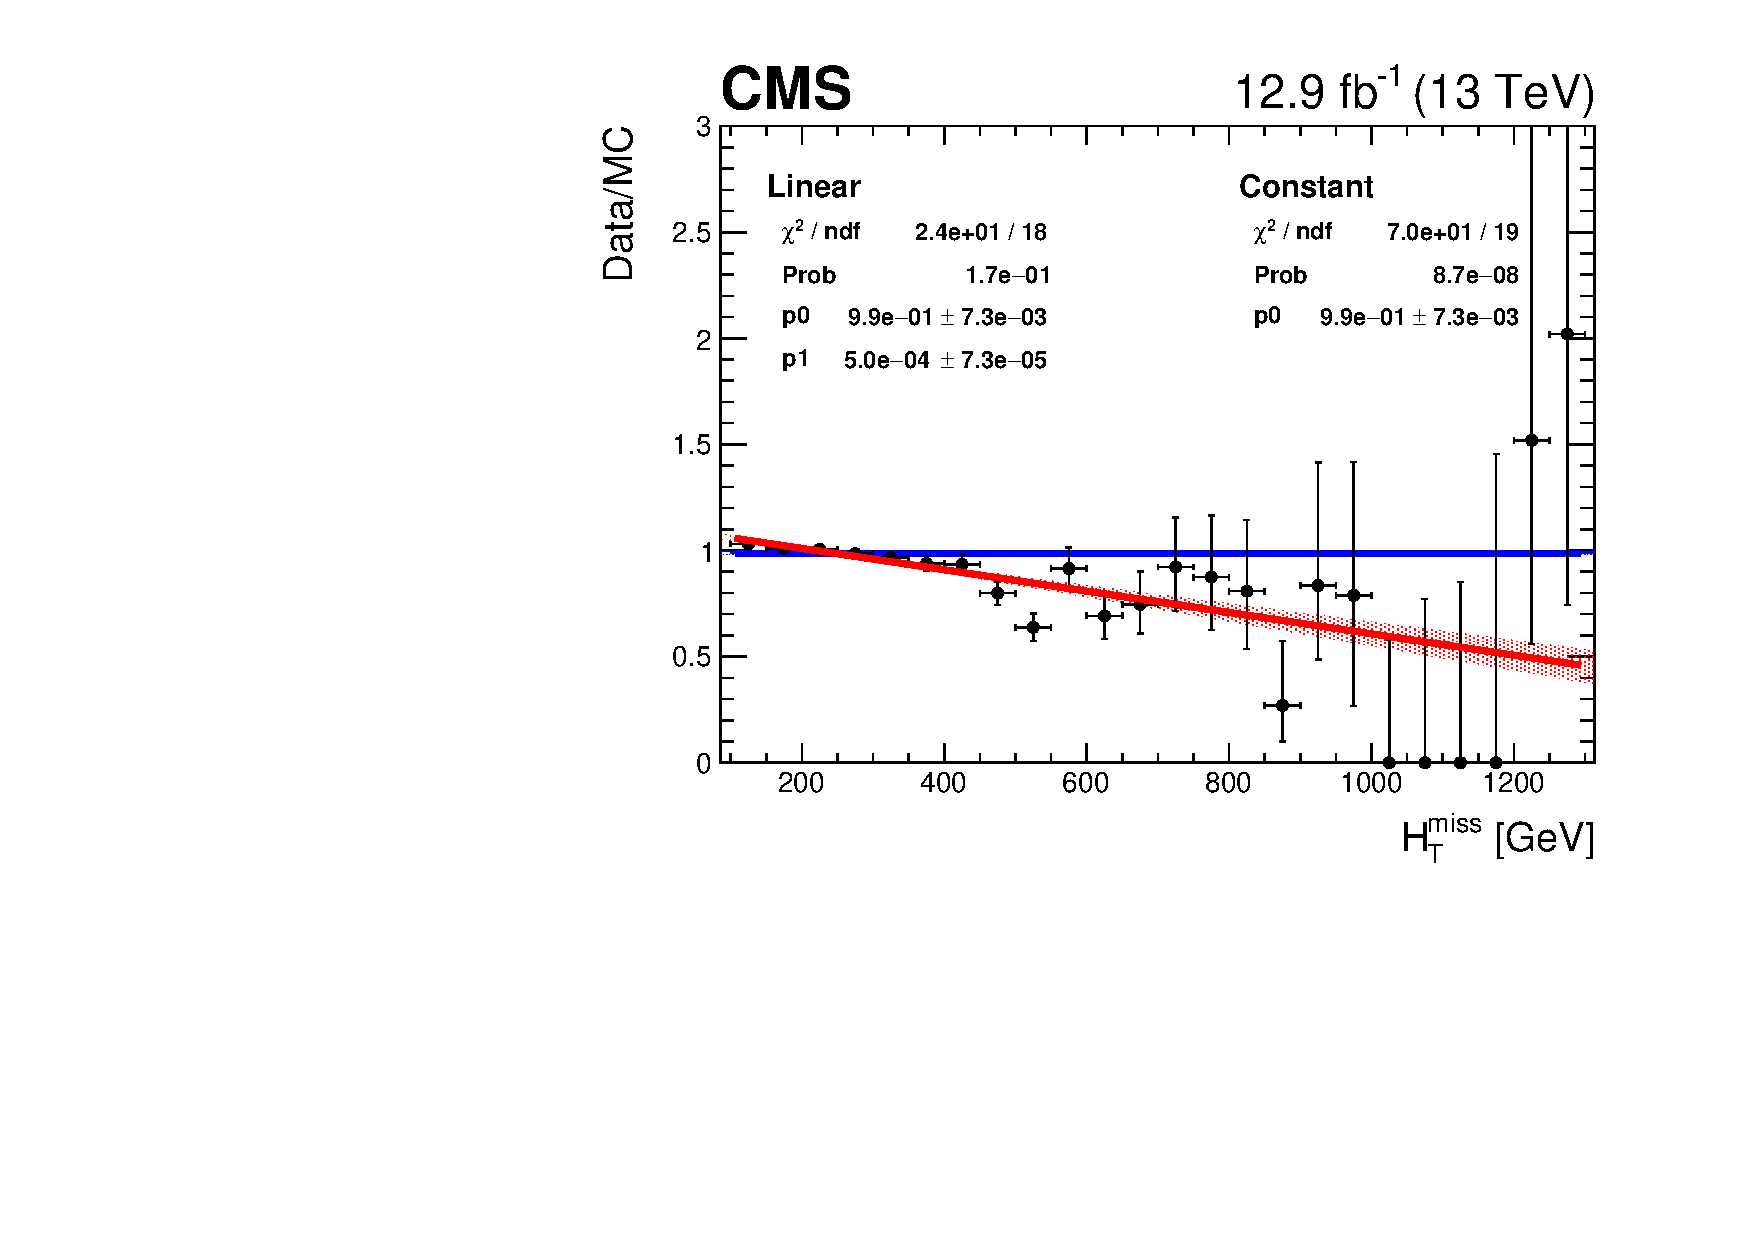
\includegraphics[width=0.5\textwidth]{Figures/backgroundPrediction/shapeOutput12FbInc/scale_ht_variable_mht/DoubleMu/Inc_Inc/finalFits/mht_Inc_Inc_ht_Inc_DoubleMu_Graph.pdf}
  }\\
  \caption{\label{fig:linearMotiv} 
  The data/MC distribution against \mht for an inclusive selection on category and \scalht
  showing the results of a linear fit. A large bias is observed as well as a low pValue for the constant fits. 
 }
\end{figure}

By anchoring the scale using binning in the \scalht dimension the remaining
bias is assumed to be negligible. In Fig.~\ref{fig:linearFitExamples} 
example fits of an orthogonal linear function to the data/MC ratio 
are shown for the three control regions. Comparing to the inclusive distribution 
the linear component can be seen to be compatible with the null hypothesis, 
i.e. no bias. In order to formalise this assertion 
the pull of the linear component from zero is calculated.
This pull distribution is shown for each of the three control regions in
in Fig.~\ref{fig:pulls} and can be seen in each case to have mean and sigma fairly 
consistent with zero and one respectively. 
and the uncertainty on the parameter is correctly estimated by the fit.
Fig.~\ref{fig:frenchFlagPulls} shows the distribution of the pulls 
in category and \scalht bins showing no areas of obvious bias.
The linear fits to the data/MC ratio additionally show a p-value following 
a uniform distribution between 0 and 1 as shown in Fig.~\ref{fig:pValues}.
This confirms that the linear component is reasonably compatible with zero ($p_1 = 0$), %i.e. no significant bias is observed, 

%Finally, an additional validation 
%can be seen from the p-value distribution of the constant fits
% -- should add p value of constant fit but currently not flat due to
% non guassian behaviour.

\begin{figure}[h!]
  \centering
  \subfigure[\gj, 1b, 2j category and \scalht 400-500\GeV bin]{
    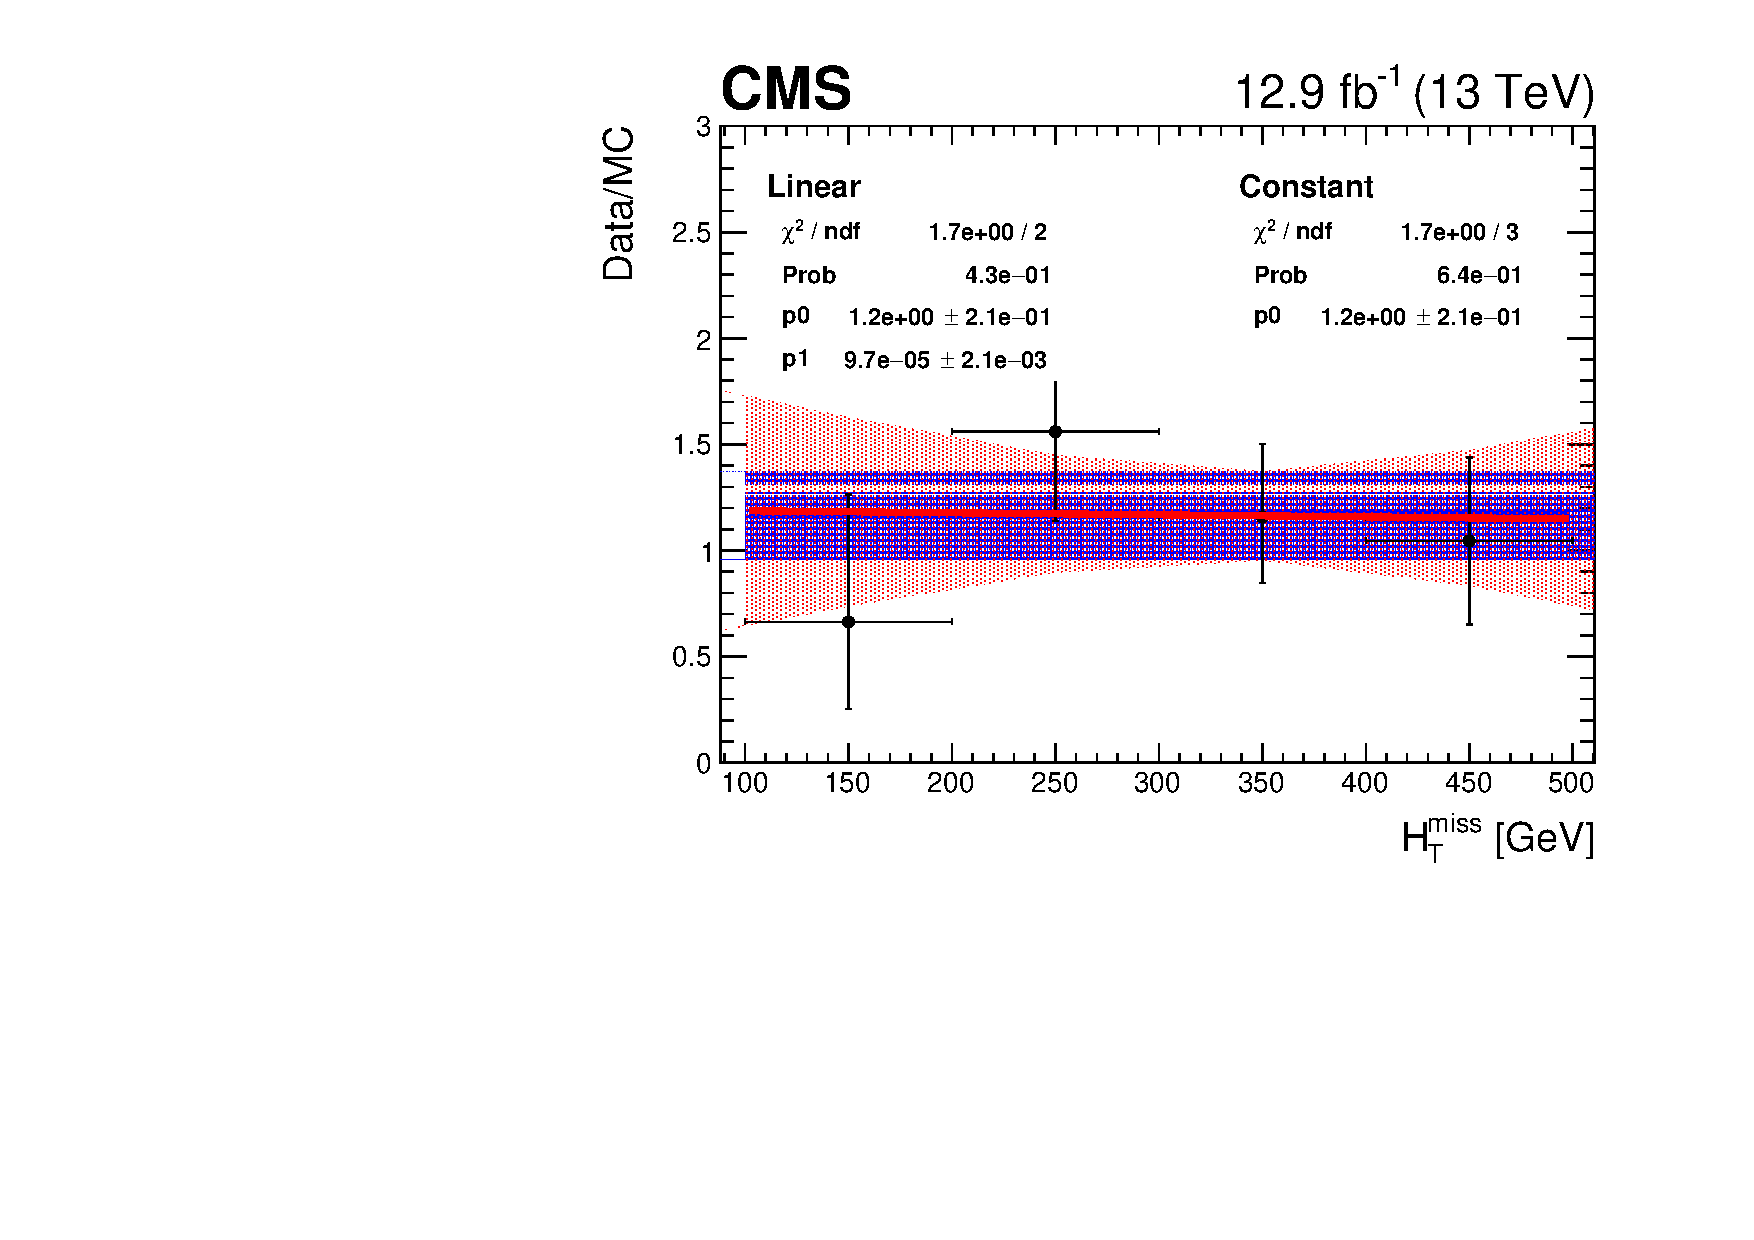
\includegraphics[width=0.5\textwidth]{Figures/backgroundPrediction/shapeOutput12Fb/scale_ht_variable_mht/representativeFits/mht_eq1b_eq2j_ht_400_500_SinglePhoton_Graph.pdf}
  }~~
  \subfigure[\mj, 1b, 4a category and \scalht 600-800\GeV bin]{
    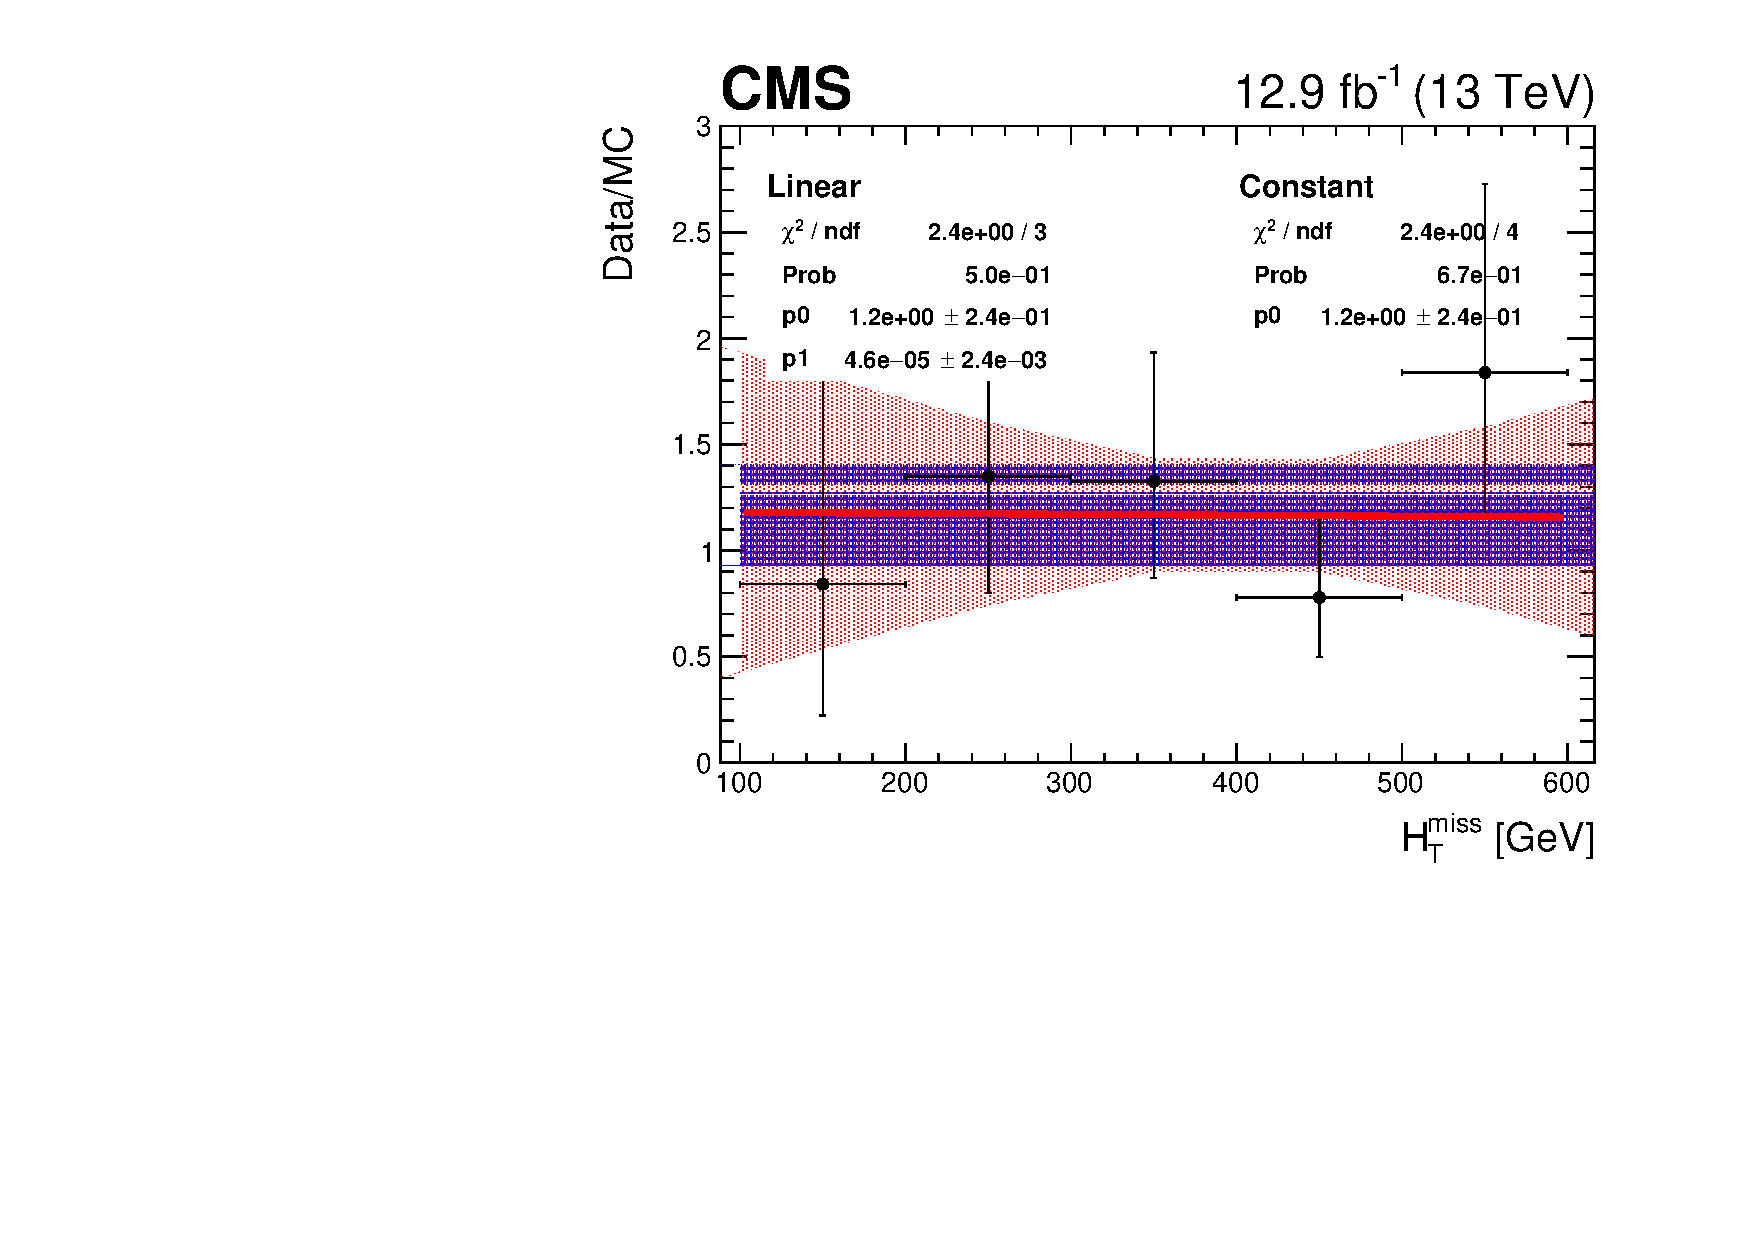
\includegraphics[width=0.5\textwidth]{Figures/backgroundPrediction/shapeOutput12Fb/scale_ht_variable_mht/representativeFits/mht_eq1b_eq4a_ht_600_800_SingleMu_Graph.pdf}
  }\\
  \subfigure[\mmj, 0b, 4j category and \scalht 300-350\GeV bin]{
    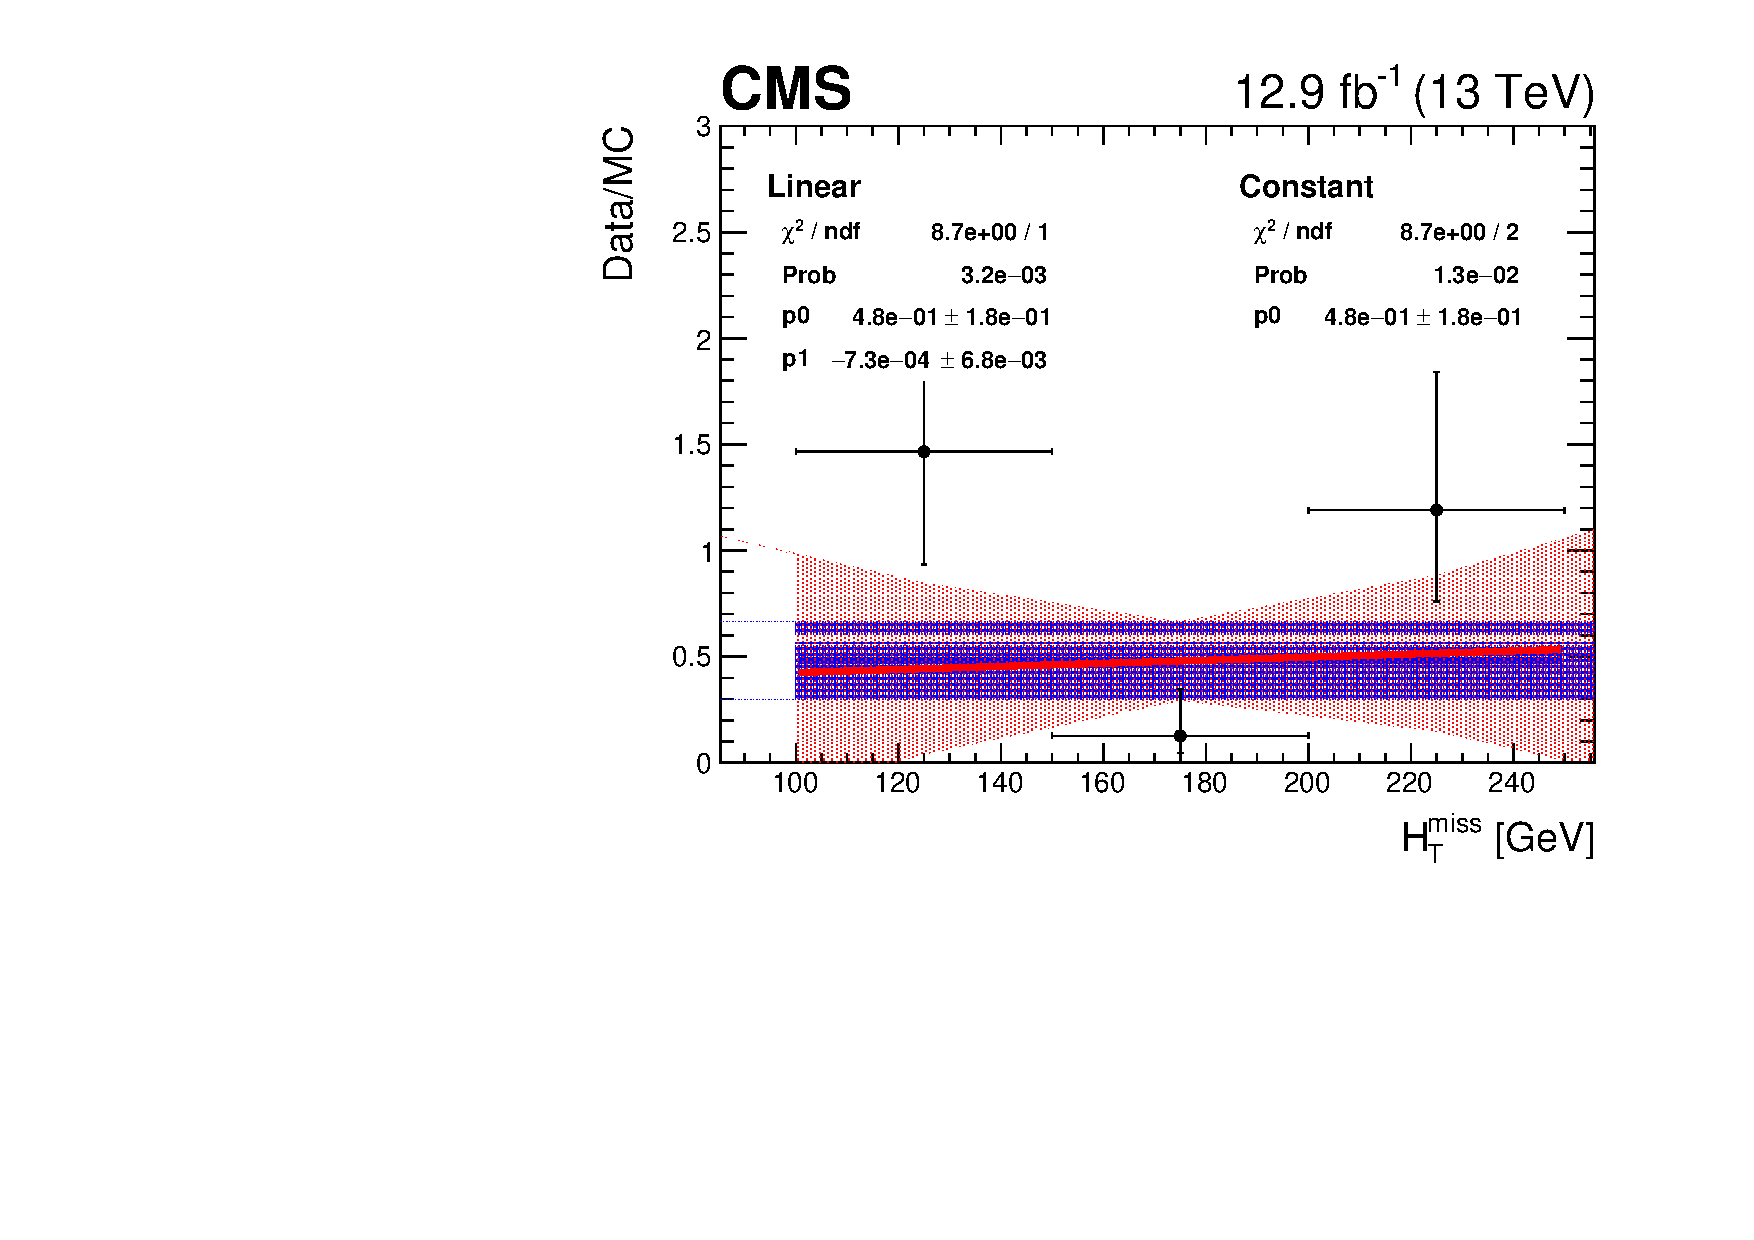
\includegraphics[width=0.5\textwidth]{Figures/backgroundPrediction/shapeOutput12Fb/scale_ht_variable_mht/representativeFits/mht_eq0b_eq4j_ht_300_350_DoubleMu_Graph.pdf}
  }~~
  \subfigure[\gj, 1b, 3j category and \scalht 600-800\GeV bin]{
    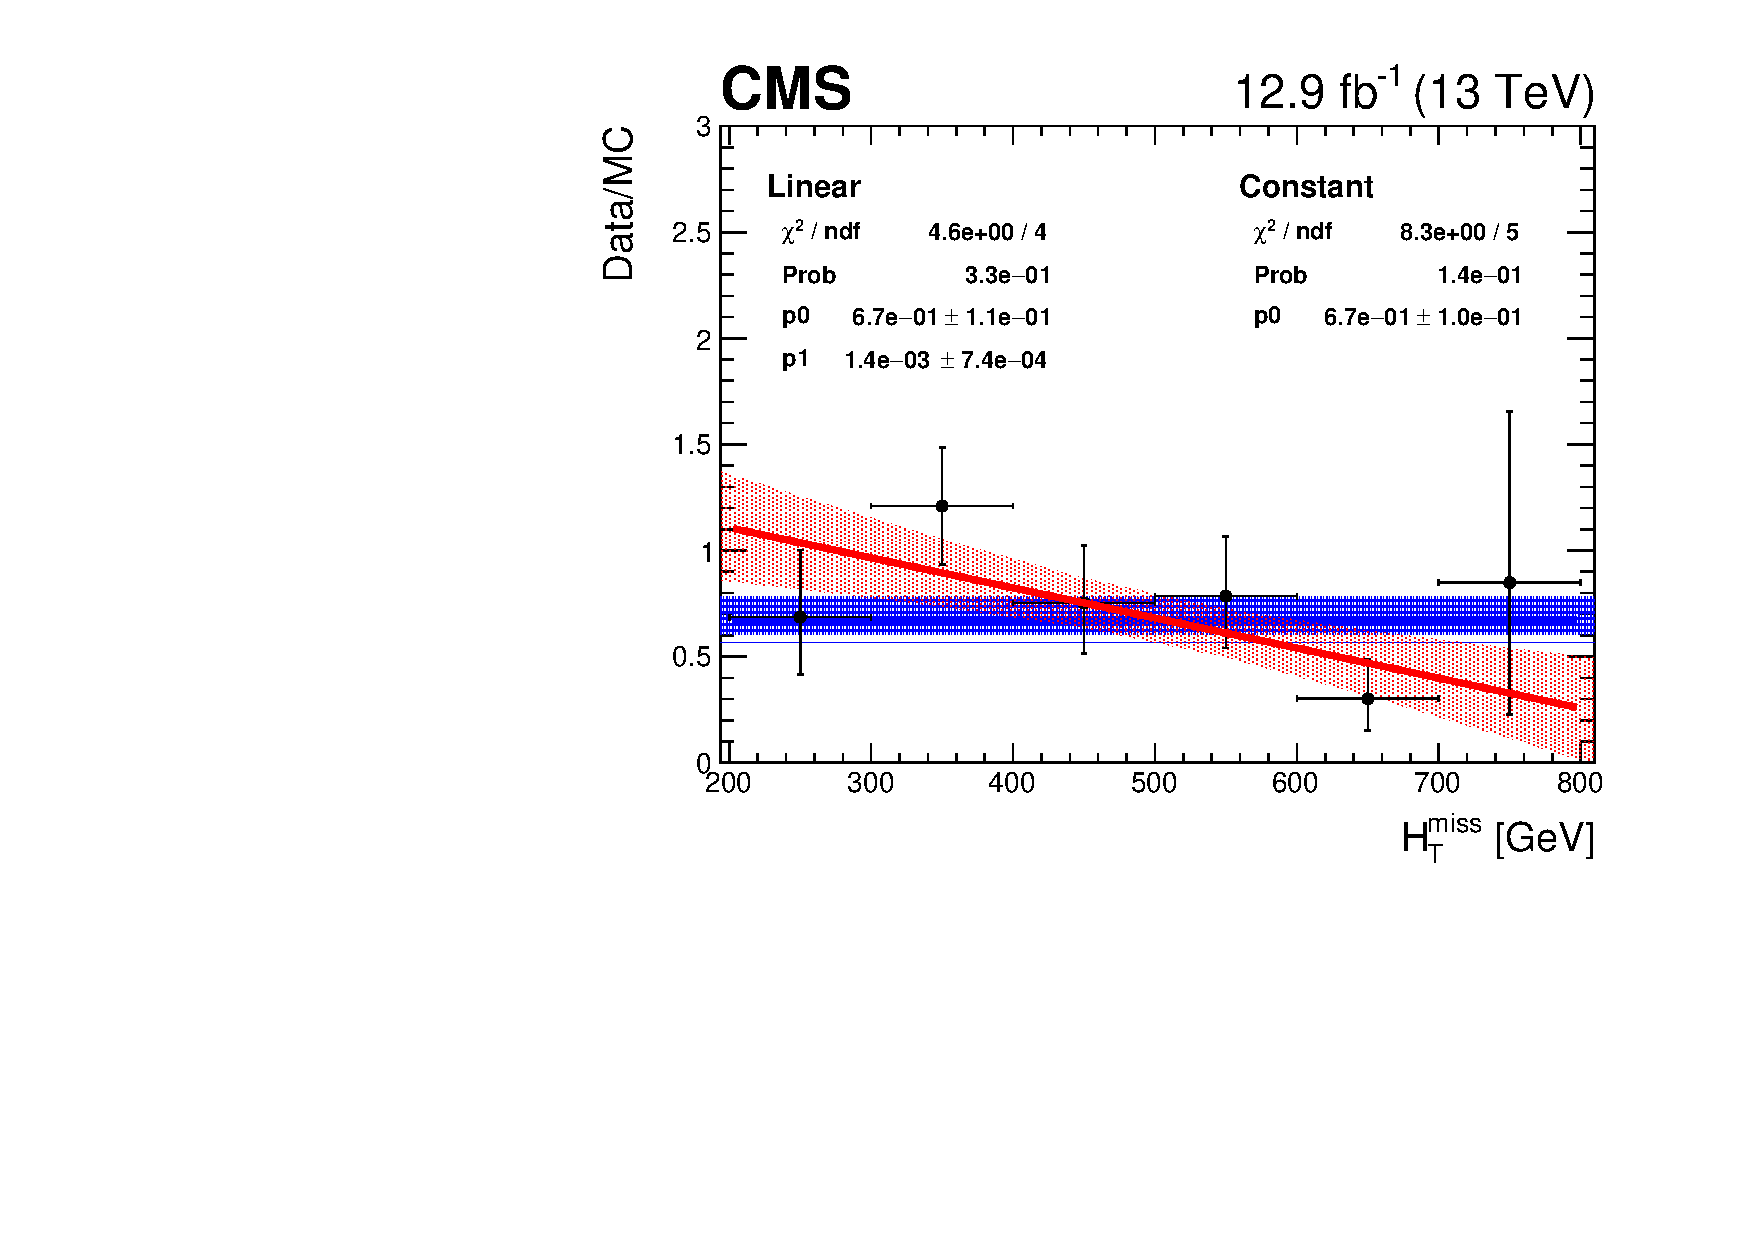
\includegraphics[width=0.5\textwidth]{Figures/backgroundPrediction/shapeOutput12Fb/scale_ht_variable_mht/SinglePhoton/eq1b_eq3j/finalFits/mht_eq1b_eq3j_ht_600_800_SinglePhoton_Graph.pdf}
  }\\
  \subfigure[\mj, 2b, 4j category and \scalht 600-800\GeV bin]{
    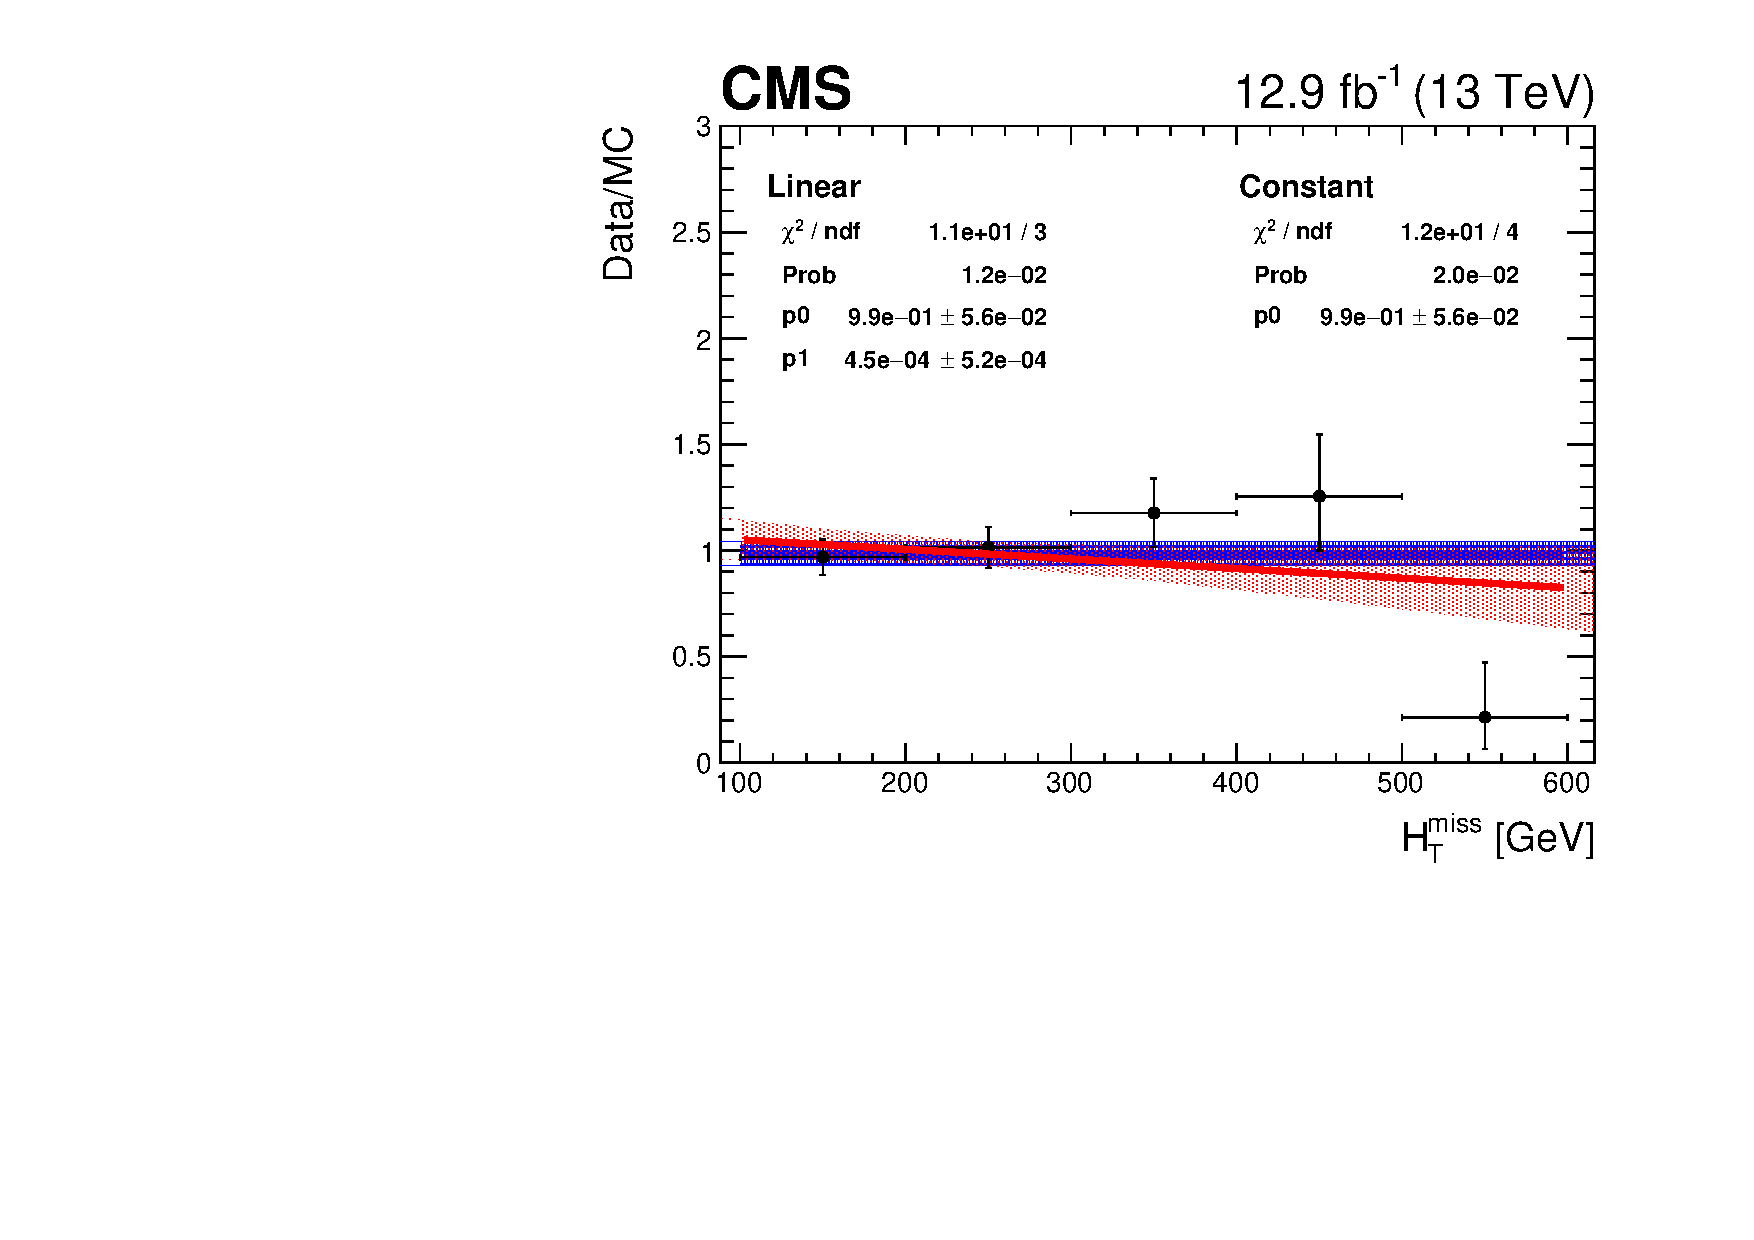
\includegraphics[width=0.5\textwidth]{Figures/backgroundPrediction/shapeOutput12Fb/scale_ht_variable_mht/SingleMu/eq2b_eq4j/finalFits/mht_eq2b_eq4j_ht_600_800_SingleMu_Graph.pdf}
  }~~
  \subfigure[\mmj, 0b, 3a category and \scalht 300-350\GeV bin]{
    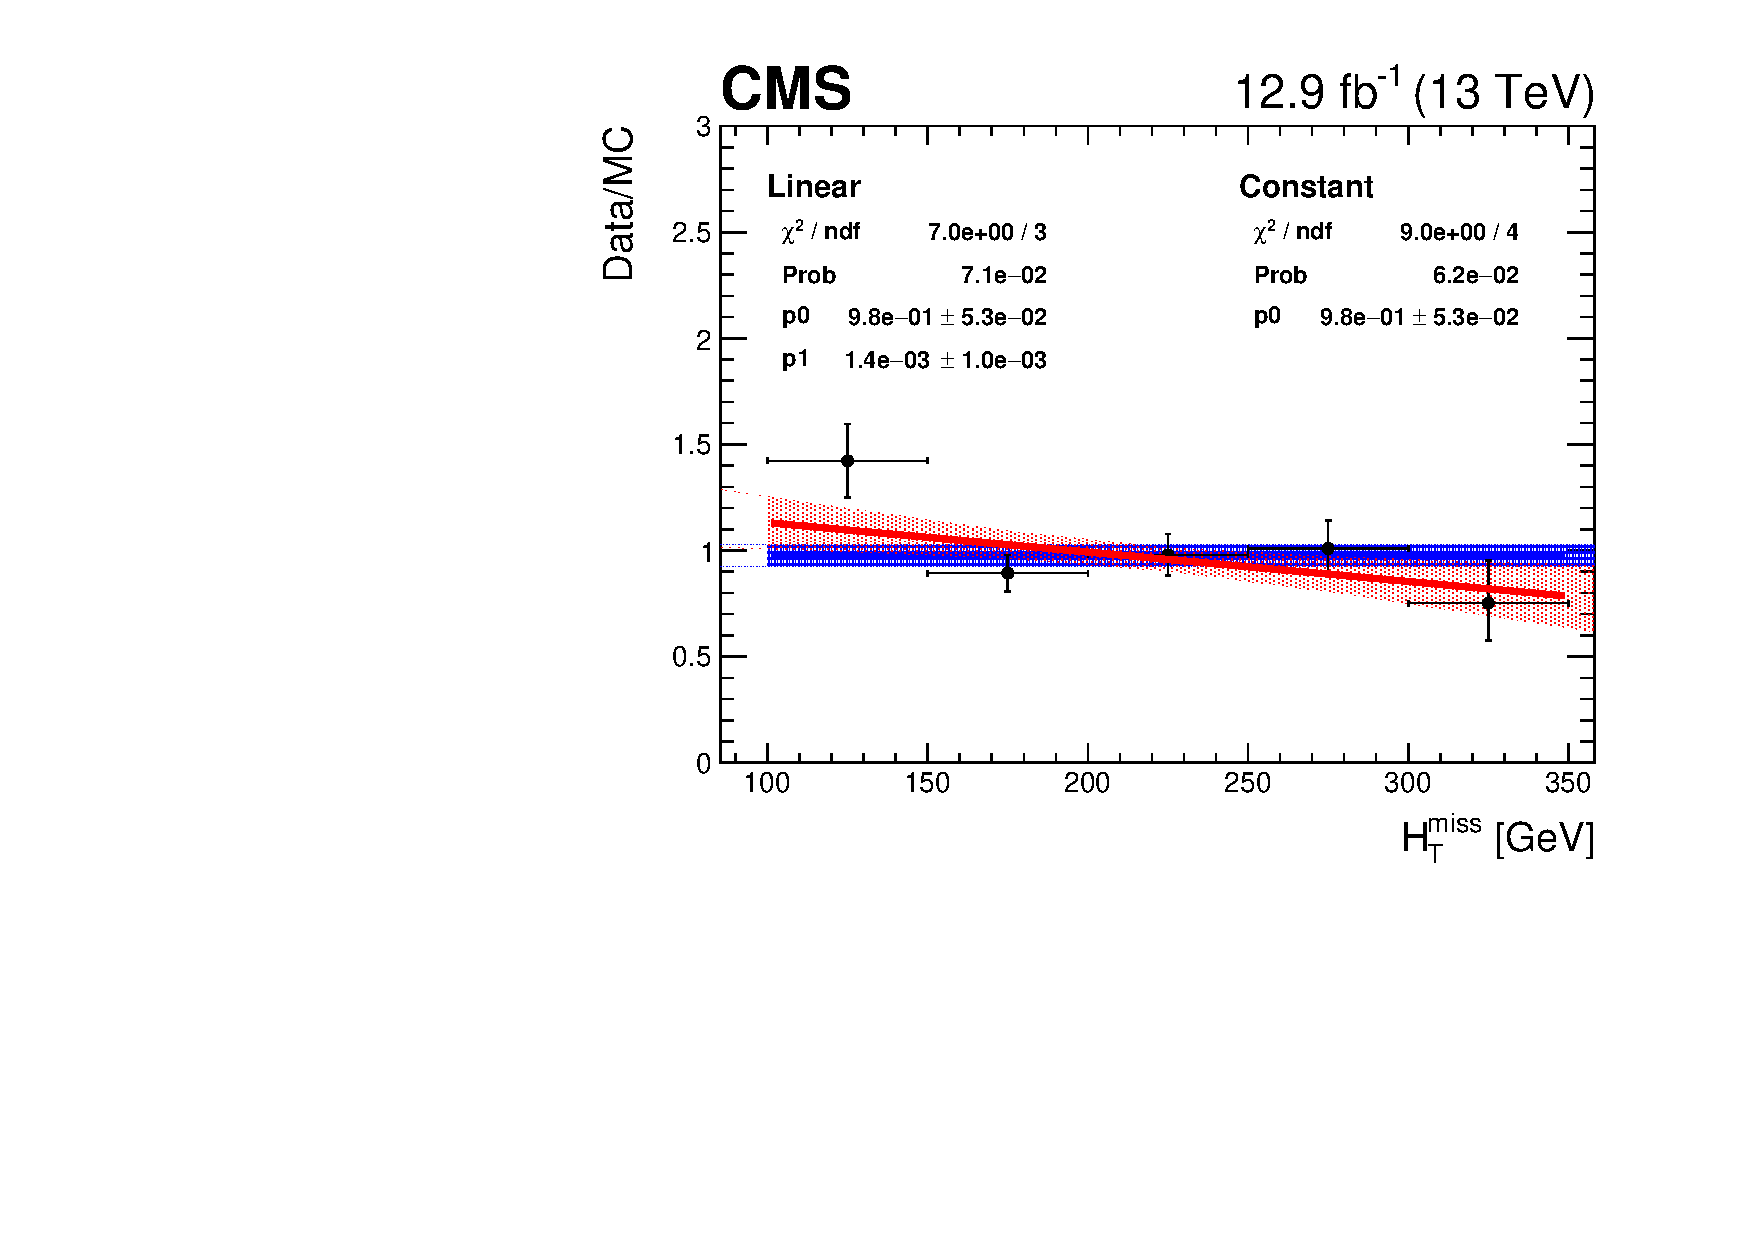
\includegraphics[width=0.5\textwidth]{Figures/backgroundPrediction/shapeOutput12Fb/scale_ht_variable_mht/DoubleMu/eq0b_eq3a/finalFits/mht_eq0b_eq3a_ht_300_350_DoubleMu_Graph.pdf}
  }\\
  \caption{\label{fig:linearFitExamples} 
  The data/MC distribution against \mht for example categories and control regions.
  The large bias in the linear component seen in Fig.~\ref{fig:linearMotiv} is mitigated.}
\end{figure}

\begin{figure}[h!]
  \centering
  \subfigure[\mj]{
    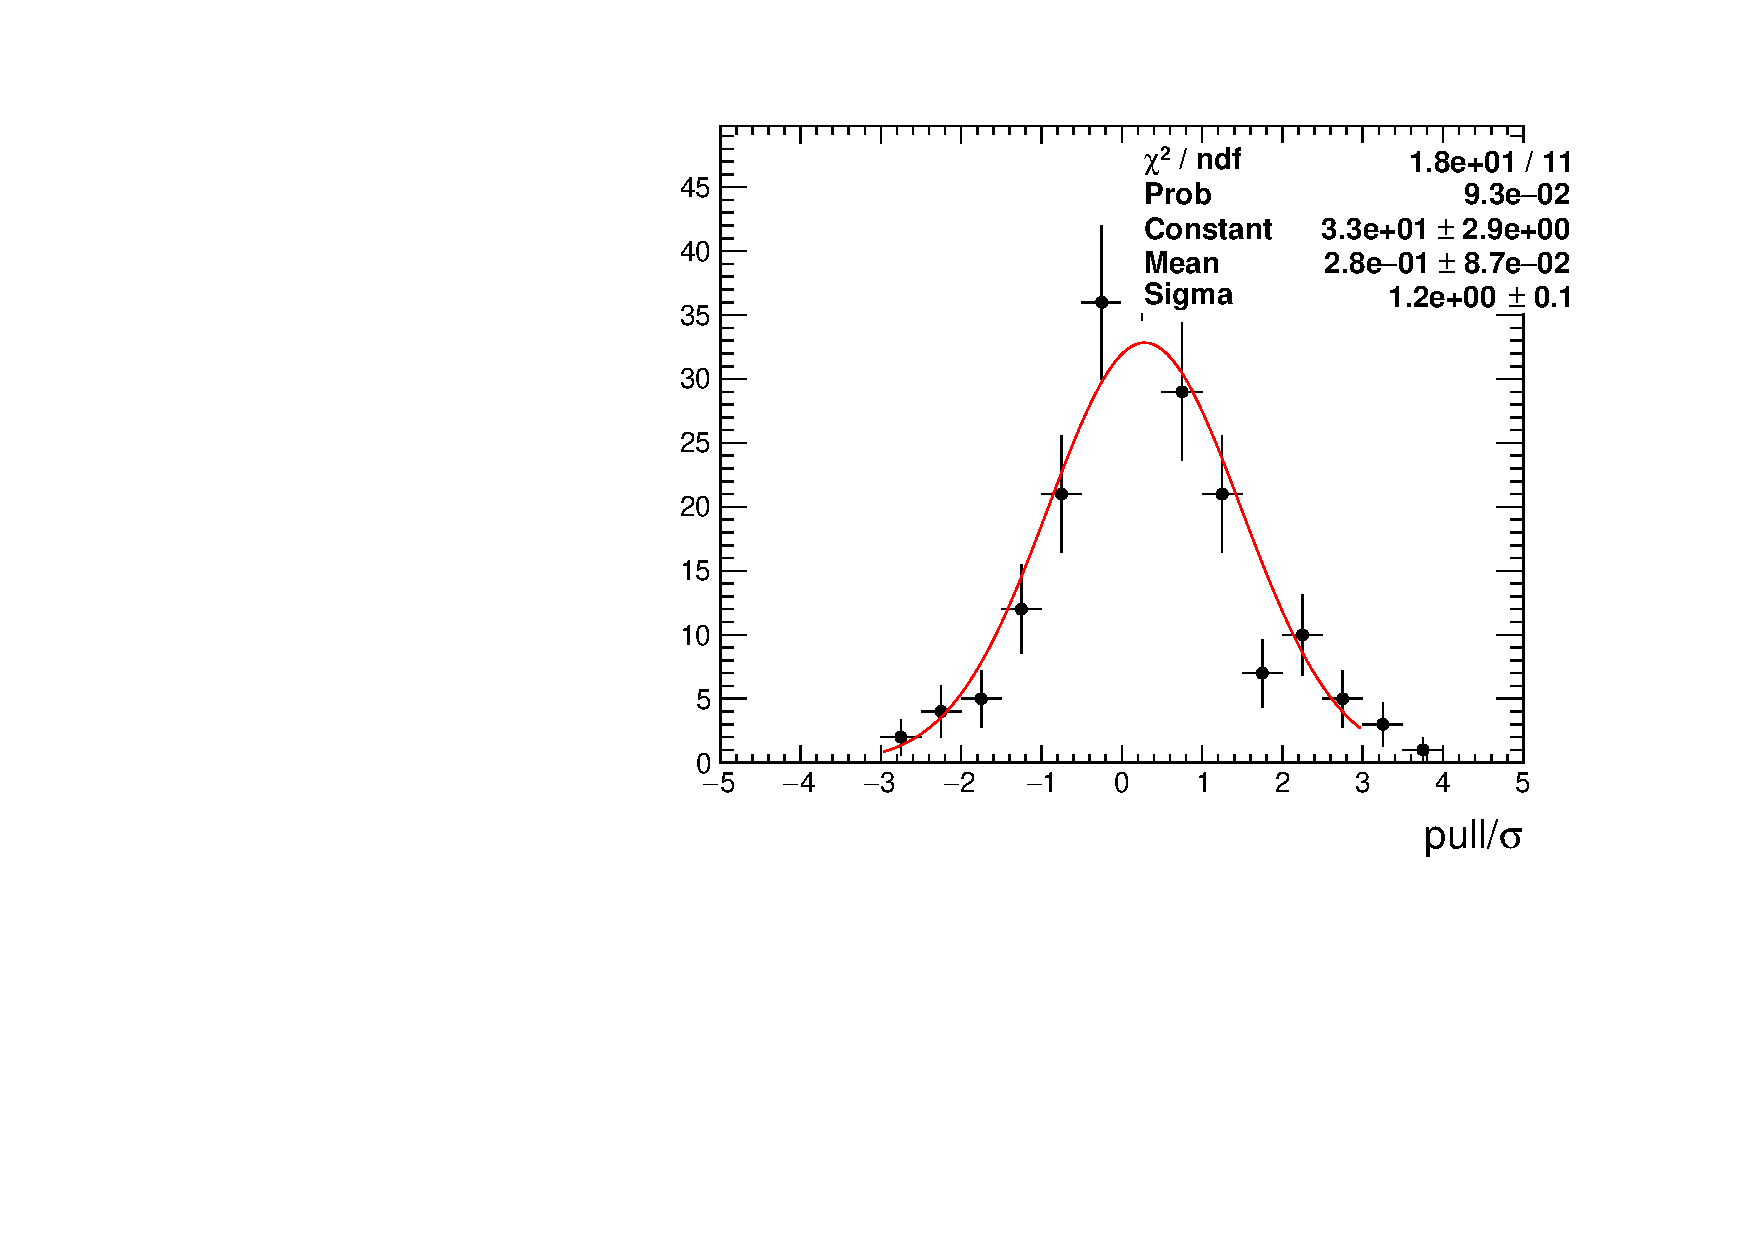
\includegraphics[width=0.5\textwidth]{Figures/backgroundPrediction/shapeOutput12Fb/scale_ht_variable_mht/SingleMu/fitOut/Linear2DShiftMean/pull_Linear2DShiftMean_p1_SingleMu.pdf}
  }~~
  \subfigure[\gj]{
    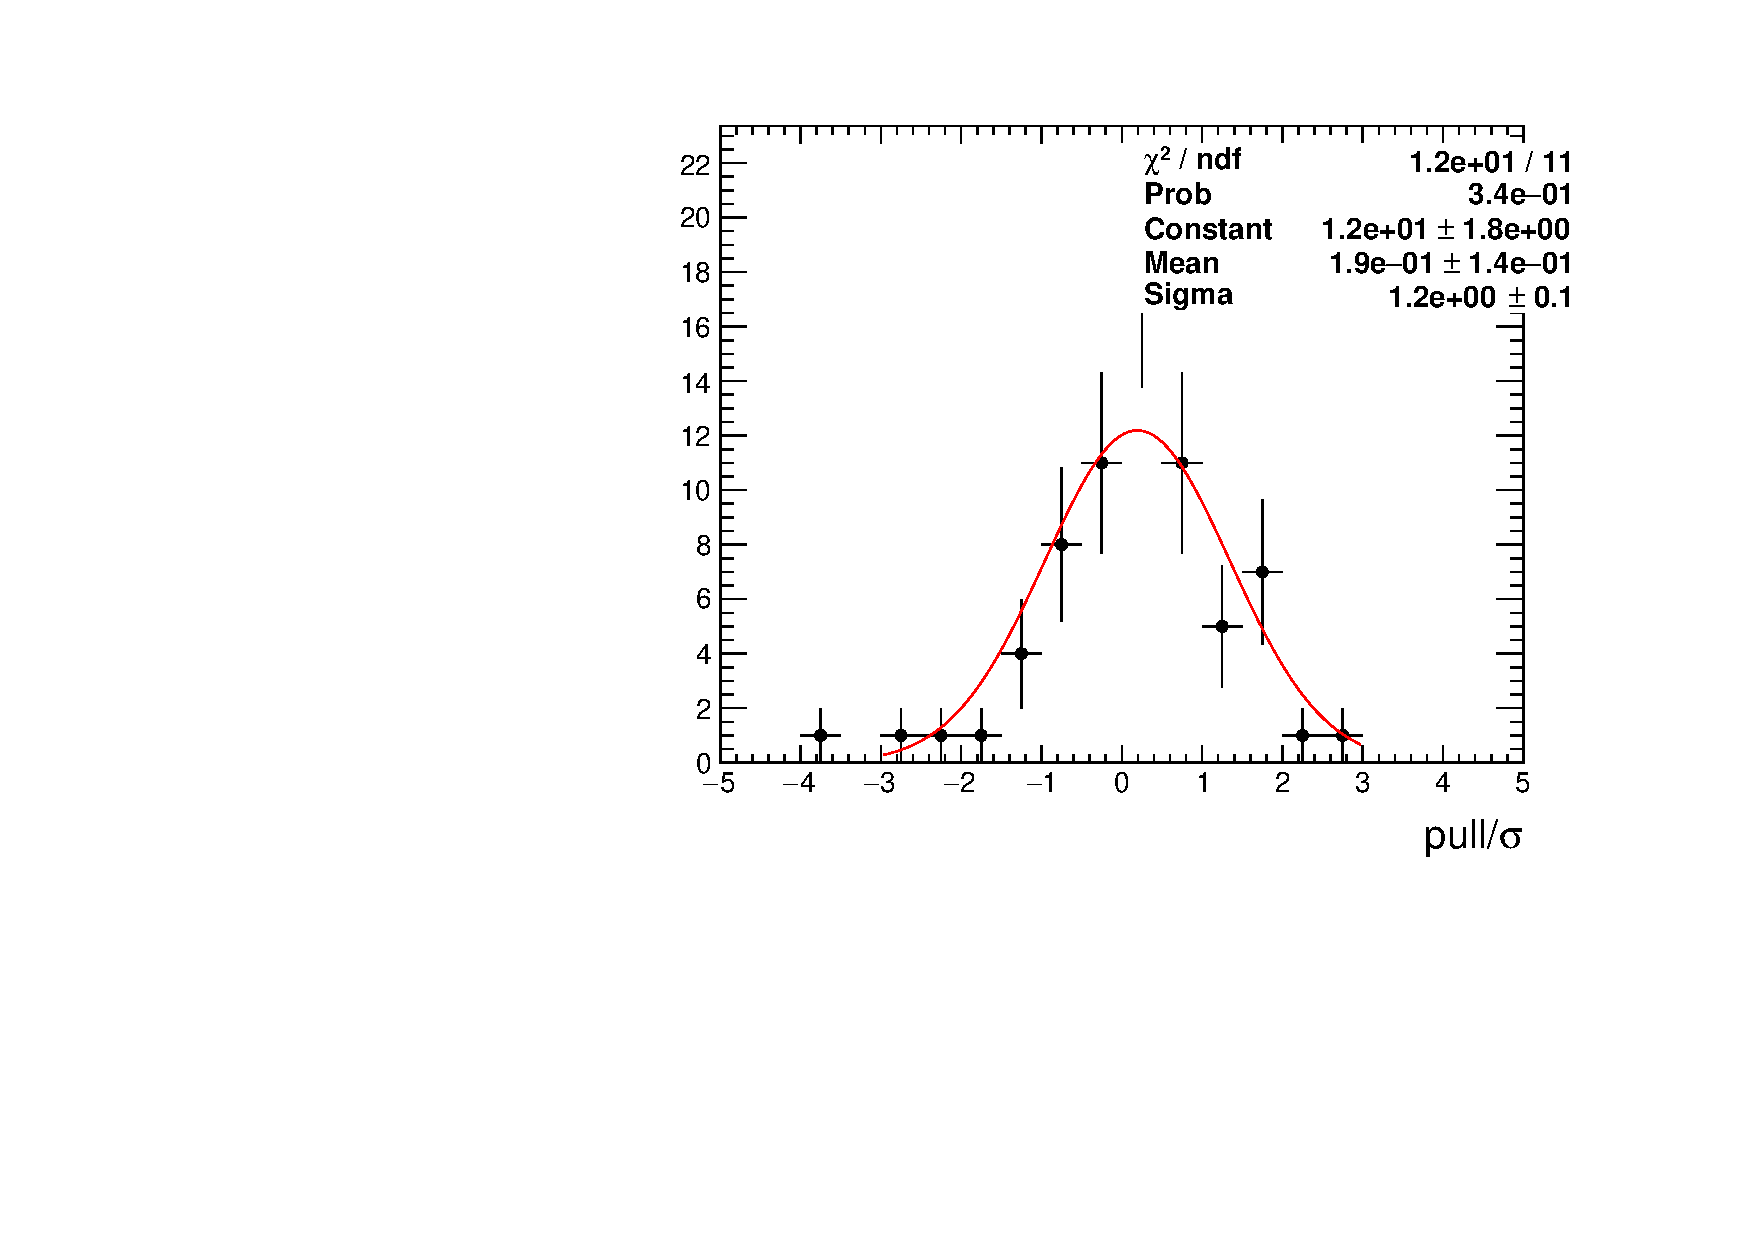
\includegraphics[width=0.5\textwidth]{Figures/backgroundPrediction/shapeOutput12Fb/scale_ht_variable_mht/SinglePhoton/fitOut/Linear2DShiftMean/pull_Linear2DShiftMean_p1_SinglePhoton.pdf}
  }\\
  \subfigure[\mmj]{
    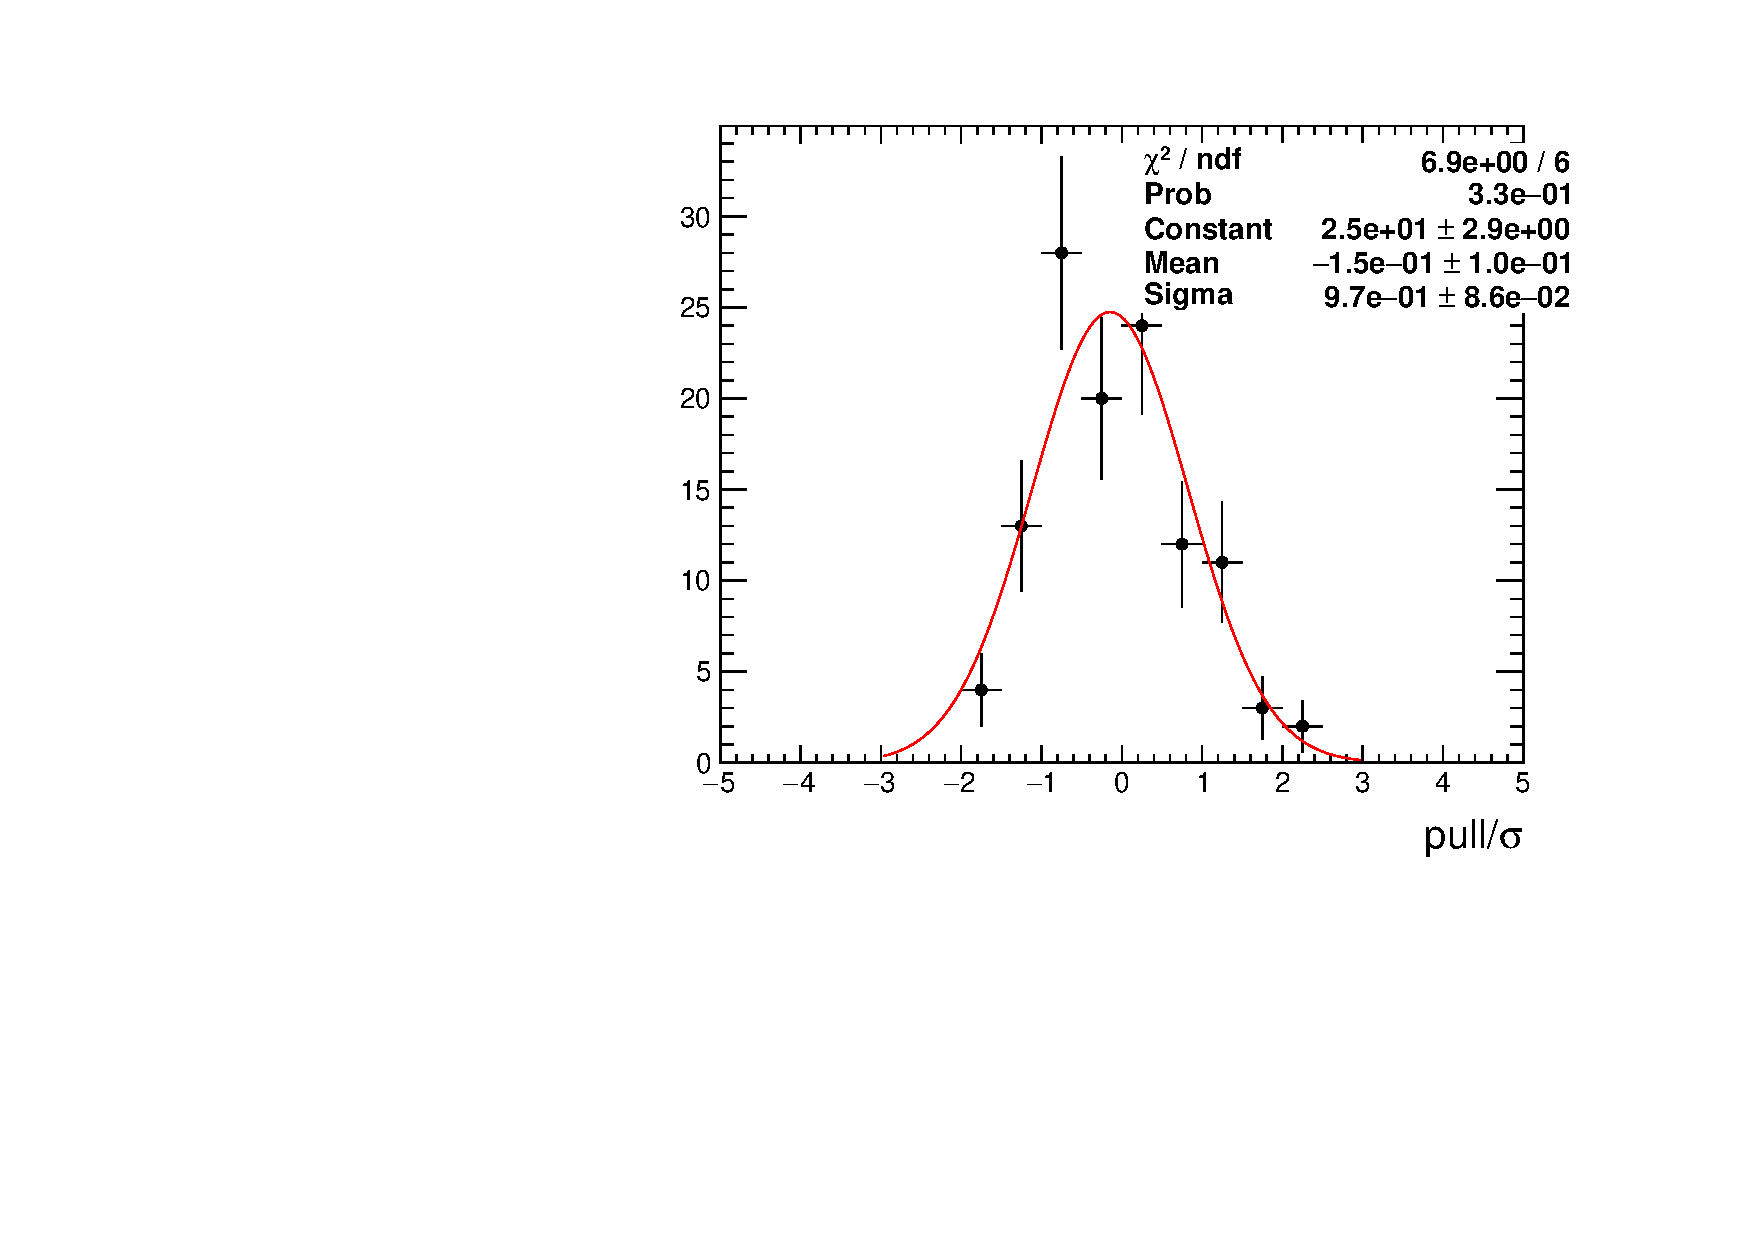
\includegraphics[width=0.5\textwidth]{Figures/backgroundPrediction/shapeOutput12Fb/scale_ht_variable_mht/DoubleMu/fitOut/Linear2DShiftMean/pull_Linear2DShiftMean_p1_DoubleMu.pdf}
  }~~
  \\
  \caption{\label{fig:pulls} 
  The pull distribution of the linear parameter from the flat hypothesis showing no significant bias.}
\end{figure}
\begin{figure}[h!]
  \centering
  \subfigure[\mj]{
    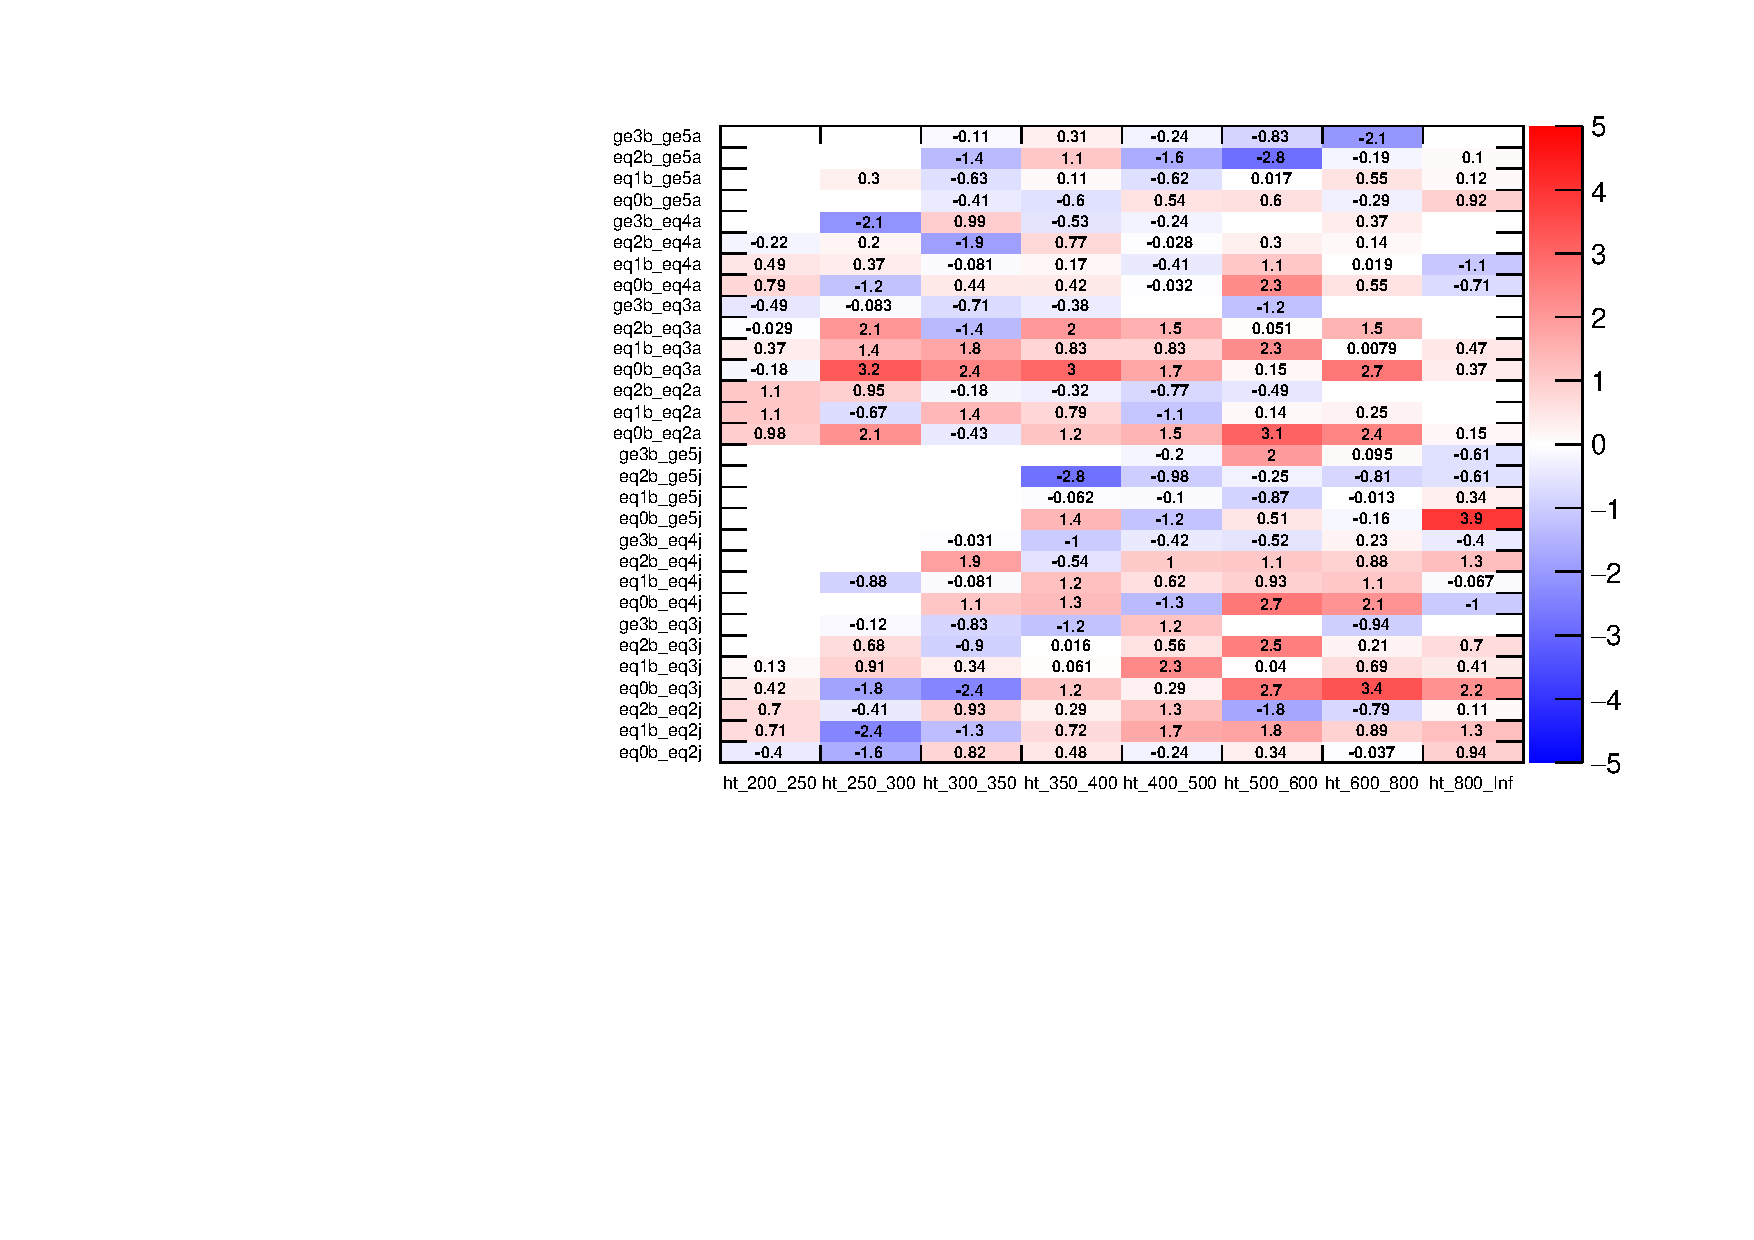
\includegraphics[width=0.5\textwidth]{Figures/backgroundPrediction/shapeOutput12Fb/scale_ht_variable_mht/SingleMu/fitOut/Linear2DShiftMean/frenchFlagPull_Linear2DShiftMean_p1_SingleMu.pdf}
  }~~
  \subfigure[\gj]{
    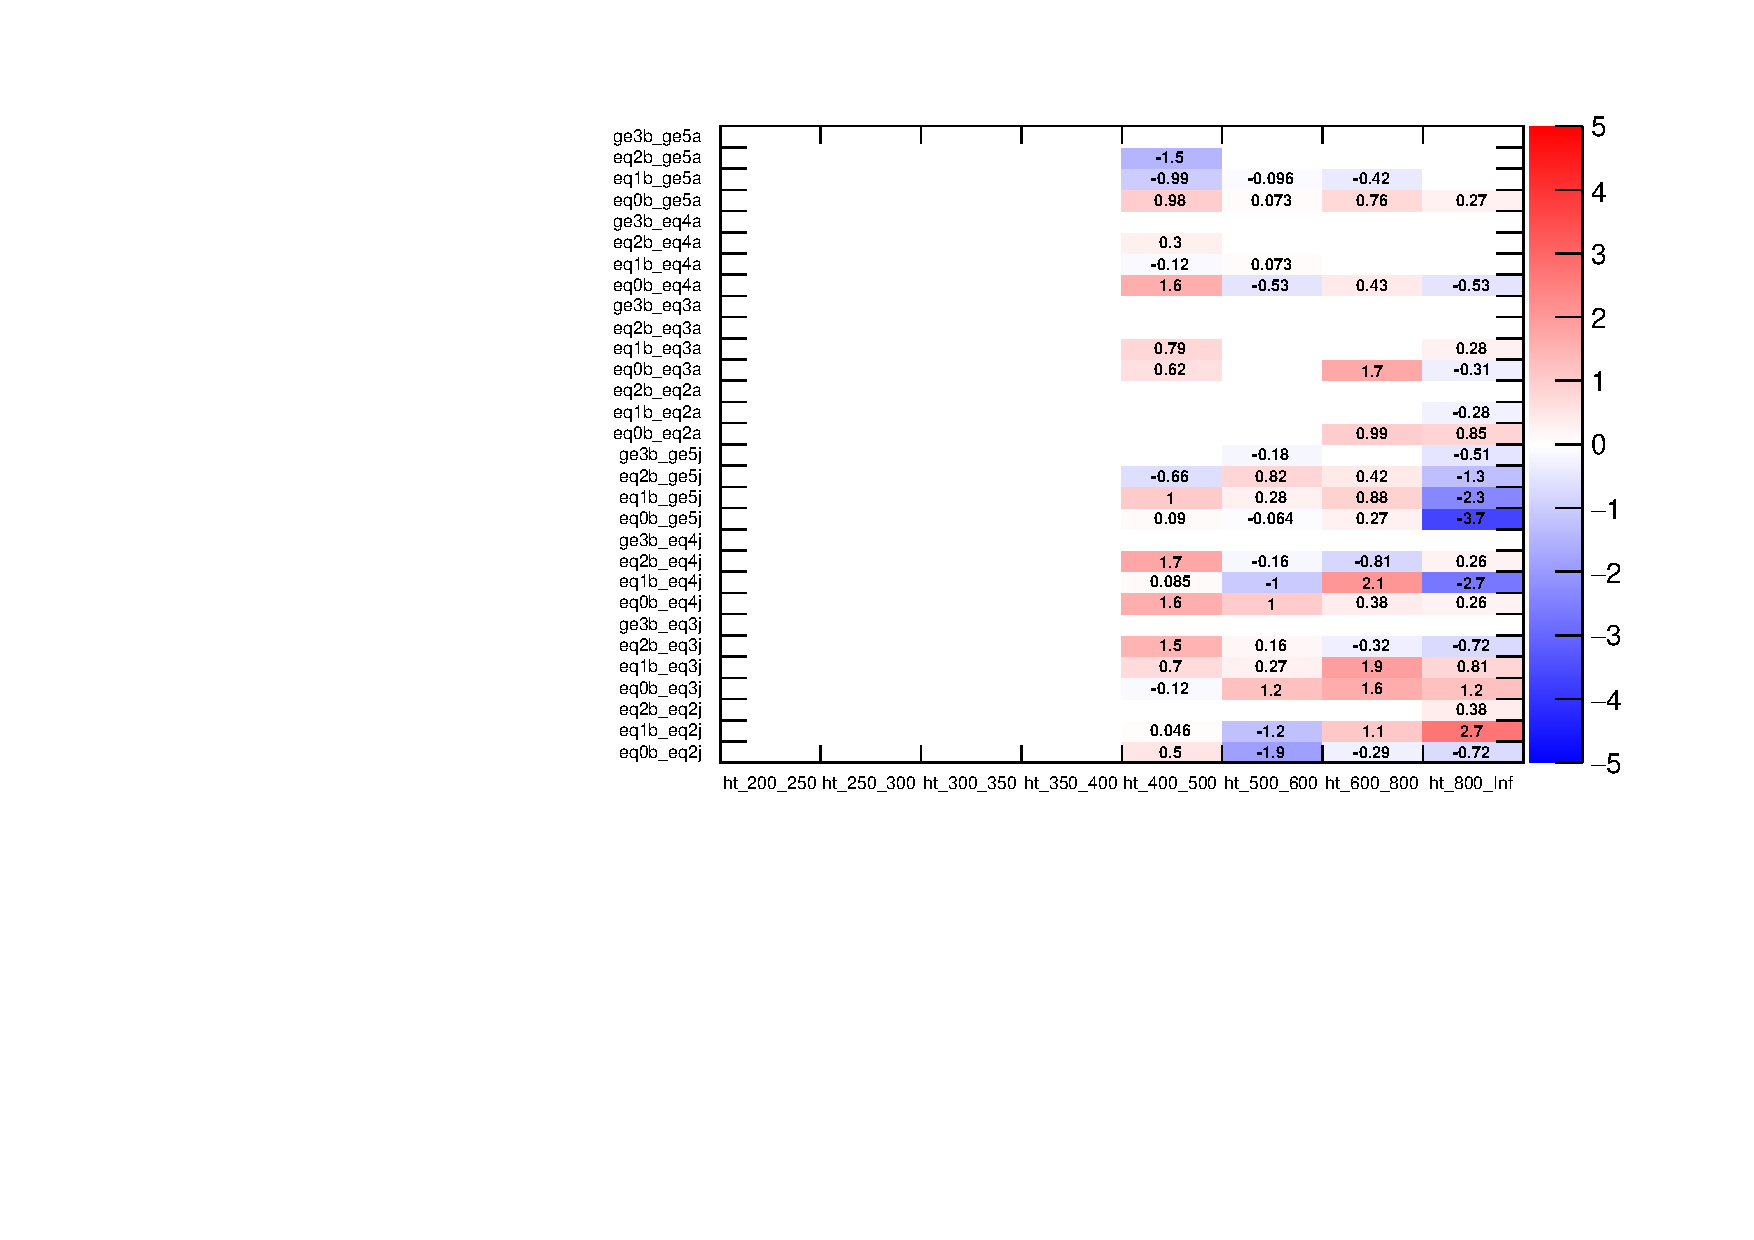
\includegraphics[width=0.5\textwidth]{Figures/backgroundPrediction/shapeOutput12Fb/scale_ht_variable_mht/SinglePhoton/fitOut/Linear2DShiftMean/frenchFlagPull_Linear2DShiftMean_p1_SinglePhoton.pdf}
  }\\
  \subfigure[\mmj]{
    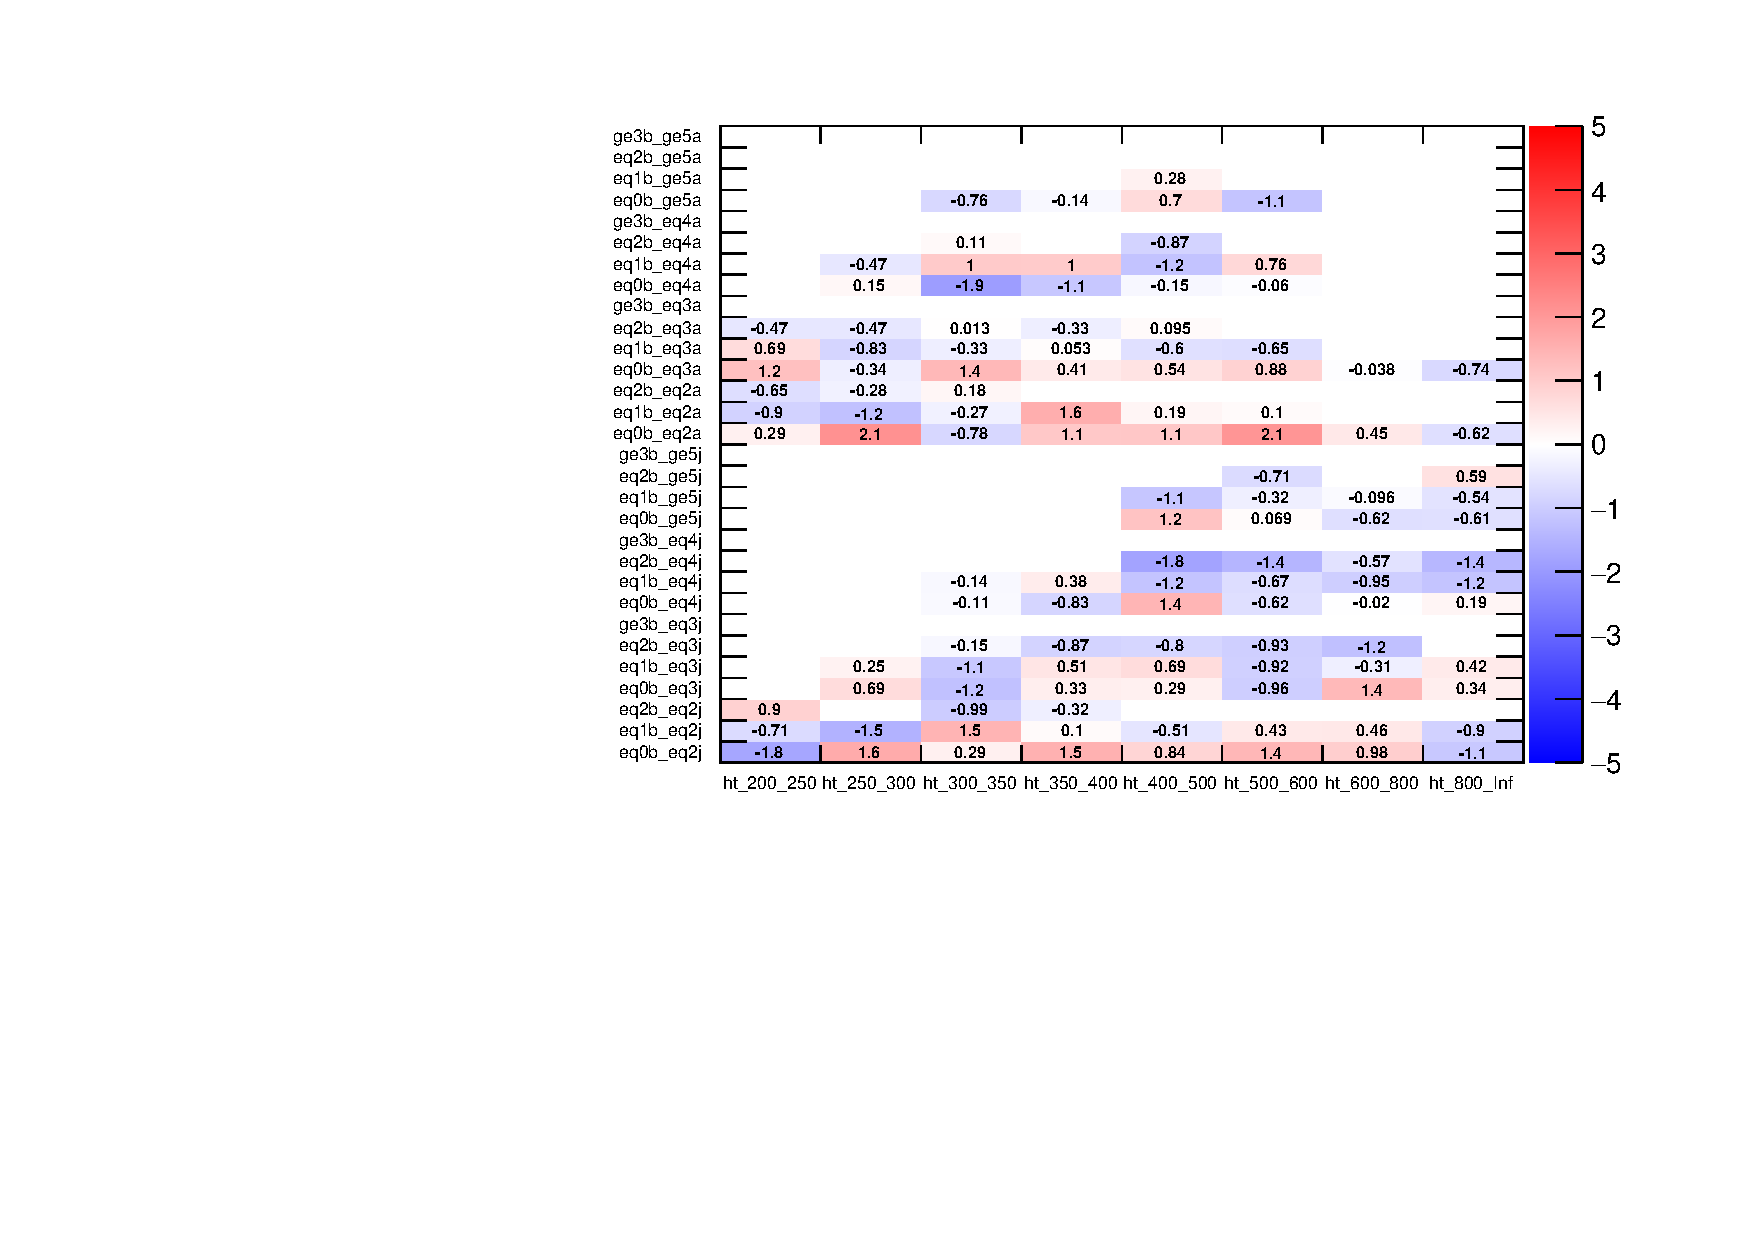
\includegraphics[width=0.5\textwidth]{Figures/backgroundPrediction/shapeOutput12Fb/scale_ht_variable_mht/DoubleMu/fitOut/Linear2DShiftMean/frenchFlagPull_Linear2DShiftMean_p1_DoubleMu.pdf}
  }~~
  \\
  \caption{\label{fig:frenchFlagPulls} The pull distribution of the linear parameter from the flat hypothesis across all
  \scalht bins and categories. There are no significant pulls for the \scalht binned
  fits while the \scalht inclusive case shows very large pulls as expected.}
\end{figure}

\begin{figure}[h!]
  \centering
  \subfigure[\mj]{
    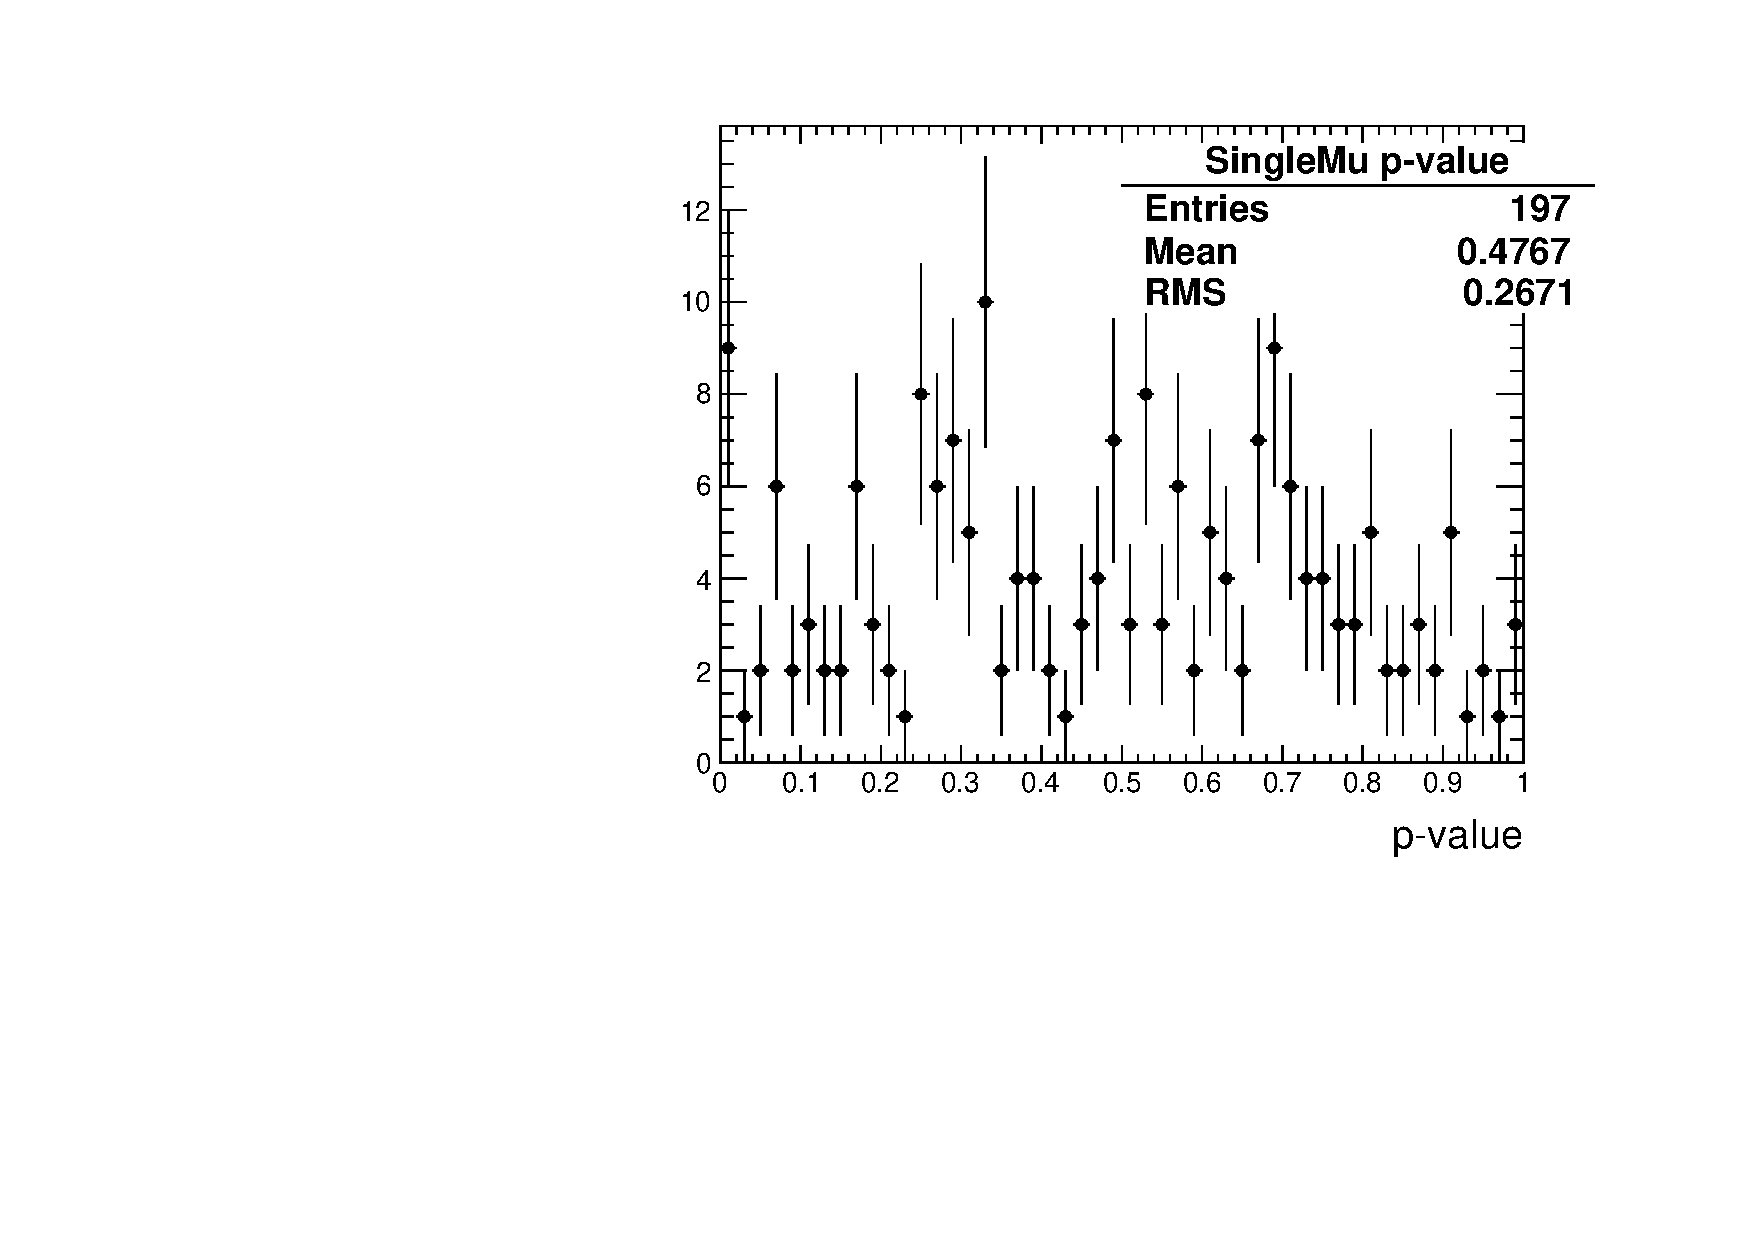
\includegraphics[width=0.5\textwidth]{Figures/backgroundPrediction/shapeOutput12Fb/scale_ht_variable_mht/SingleMu/fitOut/Linear2DShiftMean/pValue_Linear2DShiftMean_SingleMu.pdf}
  }~~
  \subfigure[\gj]{
    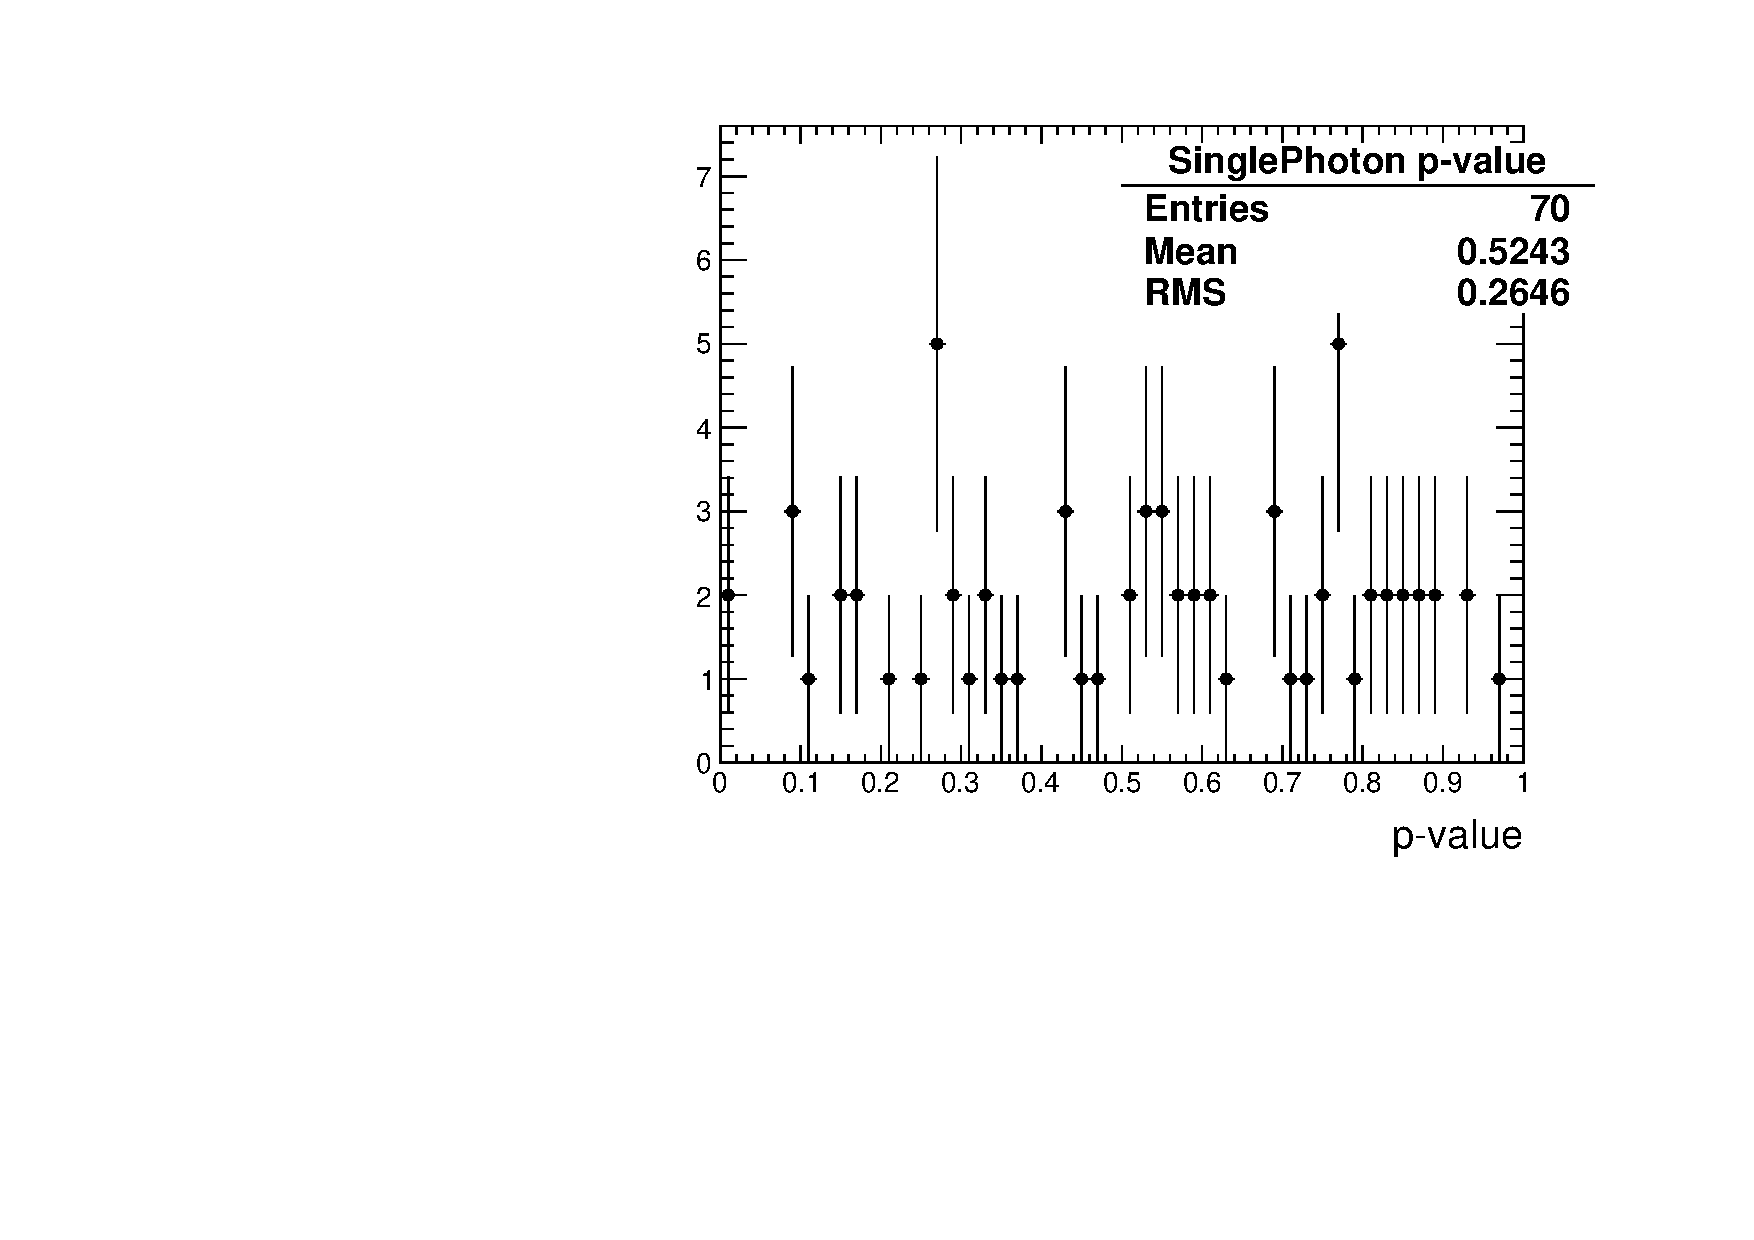
\includegraphics[width=0.5\textwidth]{Figures/backgroundPrediction/shapeOutput12Fb/scale_ht_variable_mht/SinglePhoton/fitOut/Linear2DShiftMean/pValue_Linear2DShiftMean_SinglePhoton.pdf}
  }\\
  \subfigure[\mmj]{
    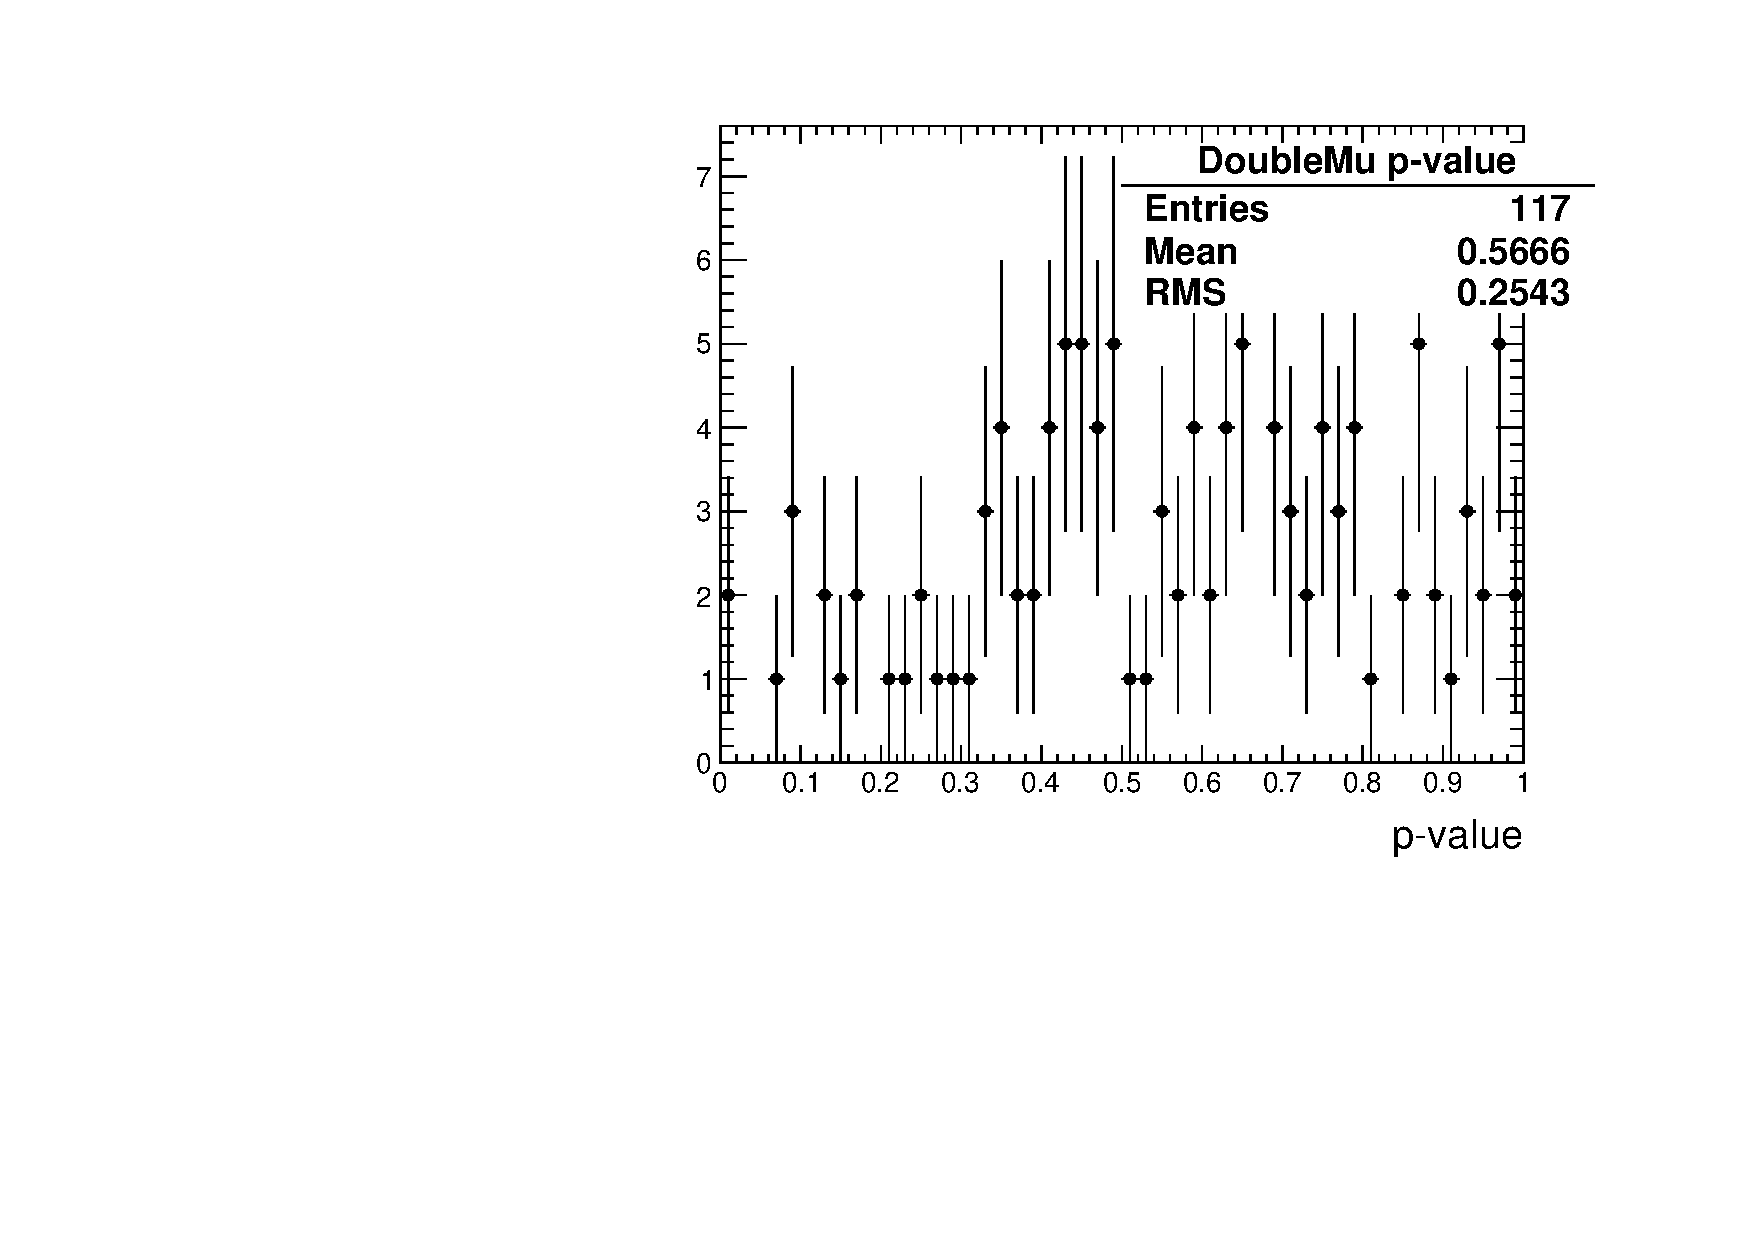
\includegraphics[width=0.5\textwidth]{Figures/backgroundPrediction/shapeOutput12Fb/scale_ht_variable_mht/DoubleMu/fitOut/Linear2DShiftMean/pValue_Linear2DShiftMean_DoubleMu.pdf}
  }~~
  \\
  \caption{\label{fig:pValues} The distributions of the p-value for the linear fit.} 
\end{figure}
\subsection{Deriving systematics on the \mht~dimension}
\label{sec:systMhtDimension}
The systematic in the \mht dimension is extracted from the hypothesis
of no bias. This is done by using the control regions 
to determine the statistical precision to which this hypothesis can
be confirmed. This information is then used to derive the systematic 
uncertainty, as described in the following. 

Each background in the signal region (\ttbar/W  and \zInv~) is predicted 
using several control regions. In order to determine the uncertainty in
the \mht dimension a combined linear fit is made over all relevant control regions
of the linear function. A requirement of at least 10 events and a non-trivial
number of degrees of freedom is made to ensure a reasonable fit. Where this
requirement is not satisfied the \mht distribution is not used in the signal region.
An \mht requirement of 130 \GeV is made to ensure a similar phase space to 
the signal region (this maps the minimum \mht due to the \alt requirements in the signal region).
The uncertainty on the linear parameter from the fit is then
used to define the up and down one sigma variations of the nominal template.
As a conservative estimate, the best fit value of the parameter is 
added in quadrature to its uncertainty in order to derive the overall variation.

Example templates with this uncertainty are shown in Fig.~\ref{fig:mht-templates-sym}, \ref{fig:mht-templates-asym} 
in Sec.~\ref{sec:results}. Here the template variations for both relevant 
backgrounds are combined to show the overall uncertainty on the \mht dimension. 
The scatter of the points around one is compatible with statistical fluctuations.

An additional validation is carried out by comparing expected and observed uncertainties
on the linear parameter defining the template variations.
The expected uncertainties are derived by using a linear fit to the MC/MC ratio where the numerator
is treated as data. The relative uncertainties per 100 \GeV from the weighted mean of \mht
for \ttbar/W and \zInv~ are shown in Fig.~\ref{fig:expectedObservedTtw} 
and Fig.~\ref{fig:expectedObservedZinv} and compared to those observed.
These show good agreement which provides additional motivation for the 
zero bias hypothesis as well as validating the method for deriving expected uncertainties.
%%%ADD WHEN UNLIND!!
% As an additional gauge of the effect of the template variations the uncertainty parameter 
% can be translate to an uncertainty on the last bin. This is typically
% of the order of 10-100\% depending on the category and is shown
% in Fig.~\ref{fig:frenchFlagLastBin}.


\begin{figure}[h!]
  \centering
  \subfigure[\label{fig:expectedTtw} Expected uncertainties]{
    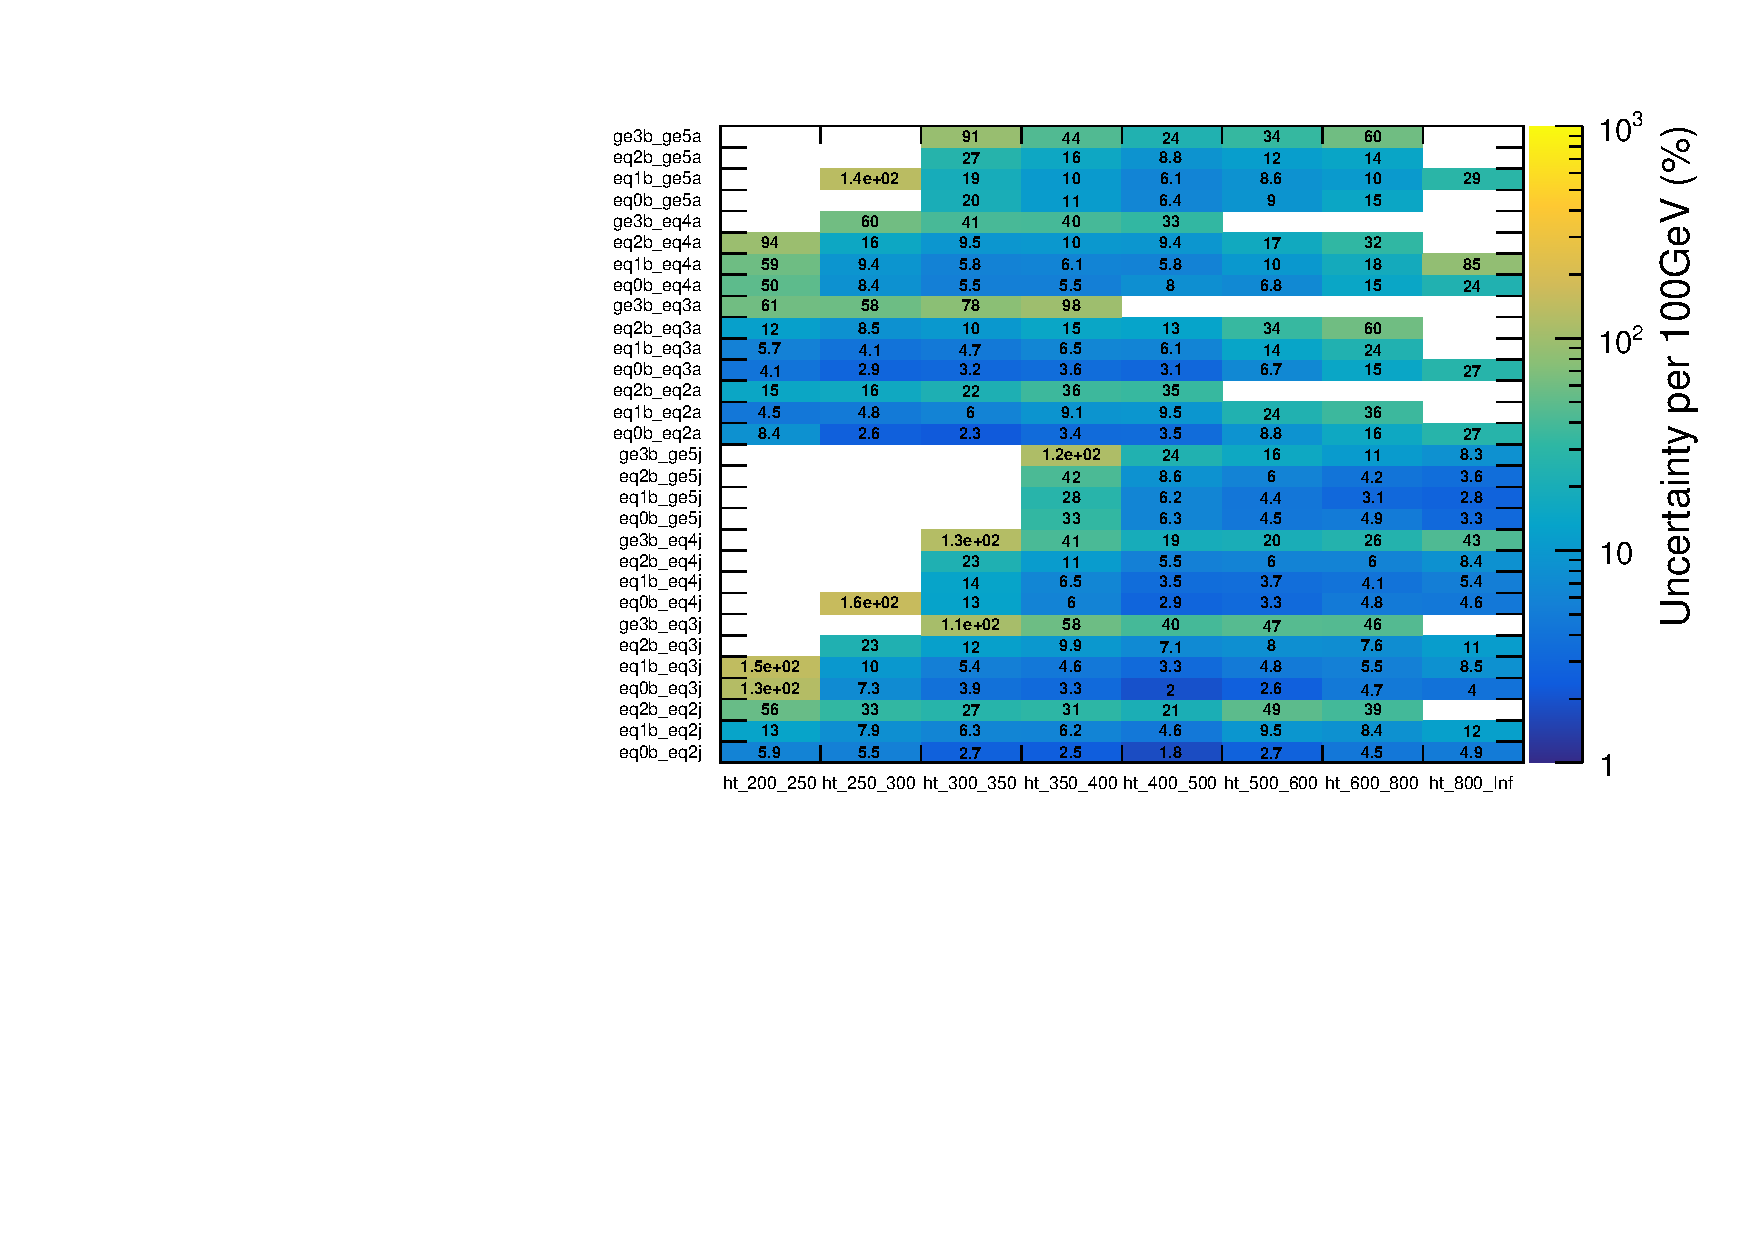
\includegraphics[width=0.5\textwidth]{Figures/backgroundPrediction/shapeOutput12FbMC/scale_ht_variable_mht/Ttw/fitOut/Linear2DShiftMean/frenchFlagErrComplete_Linear2DShiftMean_p1_Ttw.pdf}
  }~~
  \subfigure[\label{fig:observedTtw} Observed uncertainties]{
    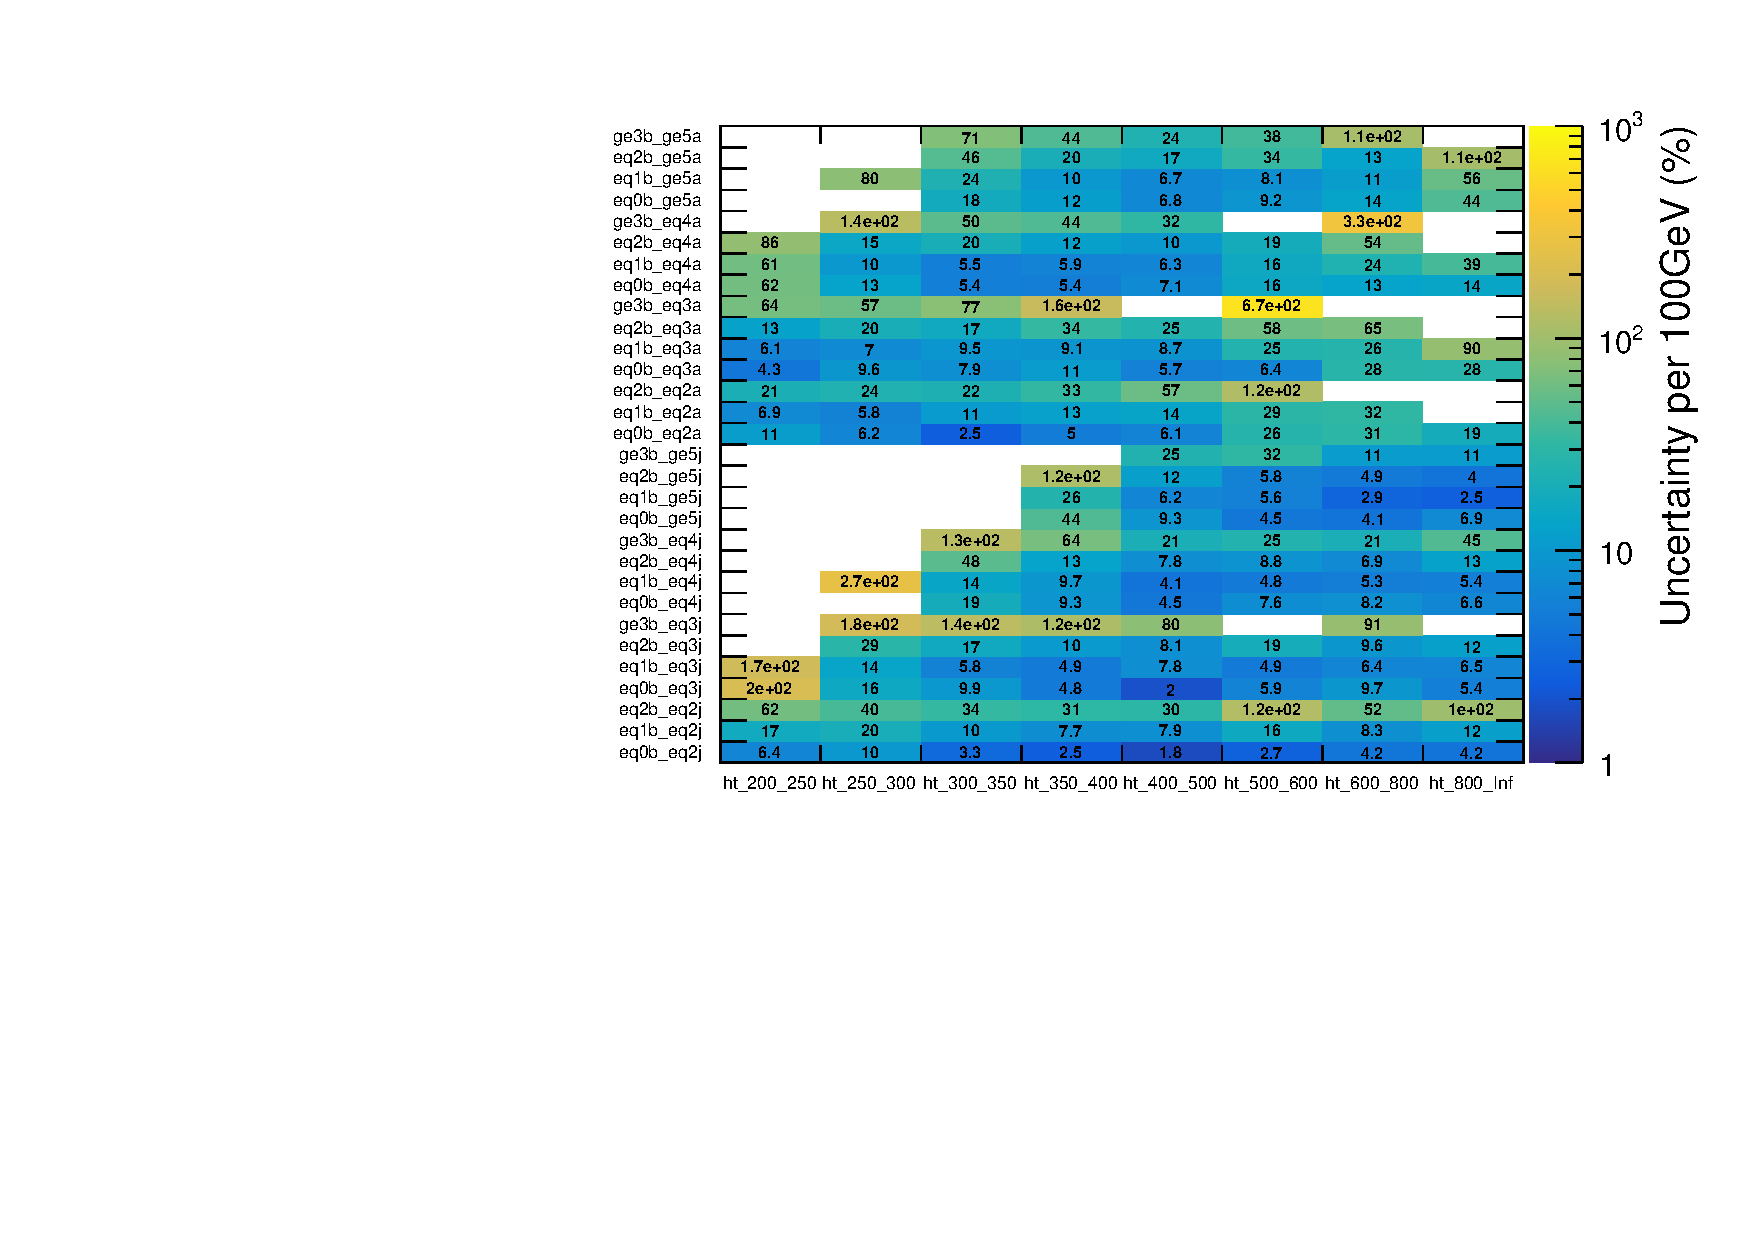
\includegraphics[width=0.5\textwidth]{Figures/backgroundPrediction/shapeOutput12Fb/scale_ht_variable_mht/Ttw/fitOut/Linear2DShiftMean/frenchFlagErrComplete_Linear2DShiftMean_p1_Ttw.pdf}
  }\\
  \caption{\label{fig:expectedObservedTtw} Expected relative uncertainties per 100 \GeV shown for \ttbar/W in Fig.~\ref{fig:expectedTtw} are consistent
  with observed uncertainties shown in Fig.~\ref{fig:observedTtw}.}
\end{figure}

\begin{figure}[h!]
  \centering
  \subfigure[\label{fig:expectedZinv} Expected uncertainties]{
    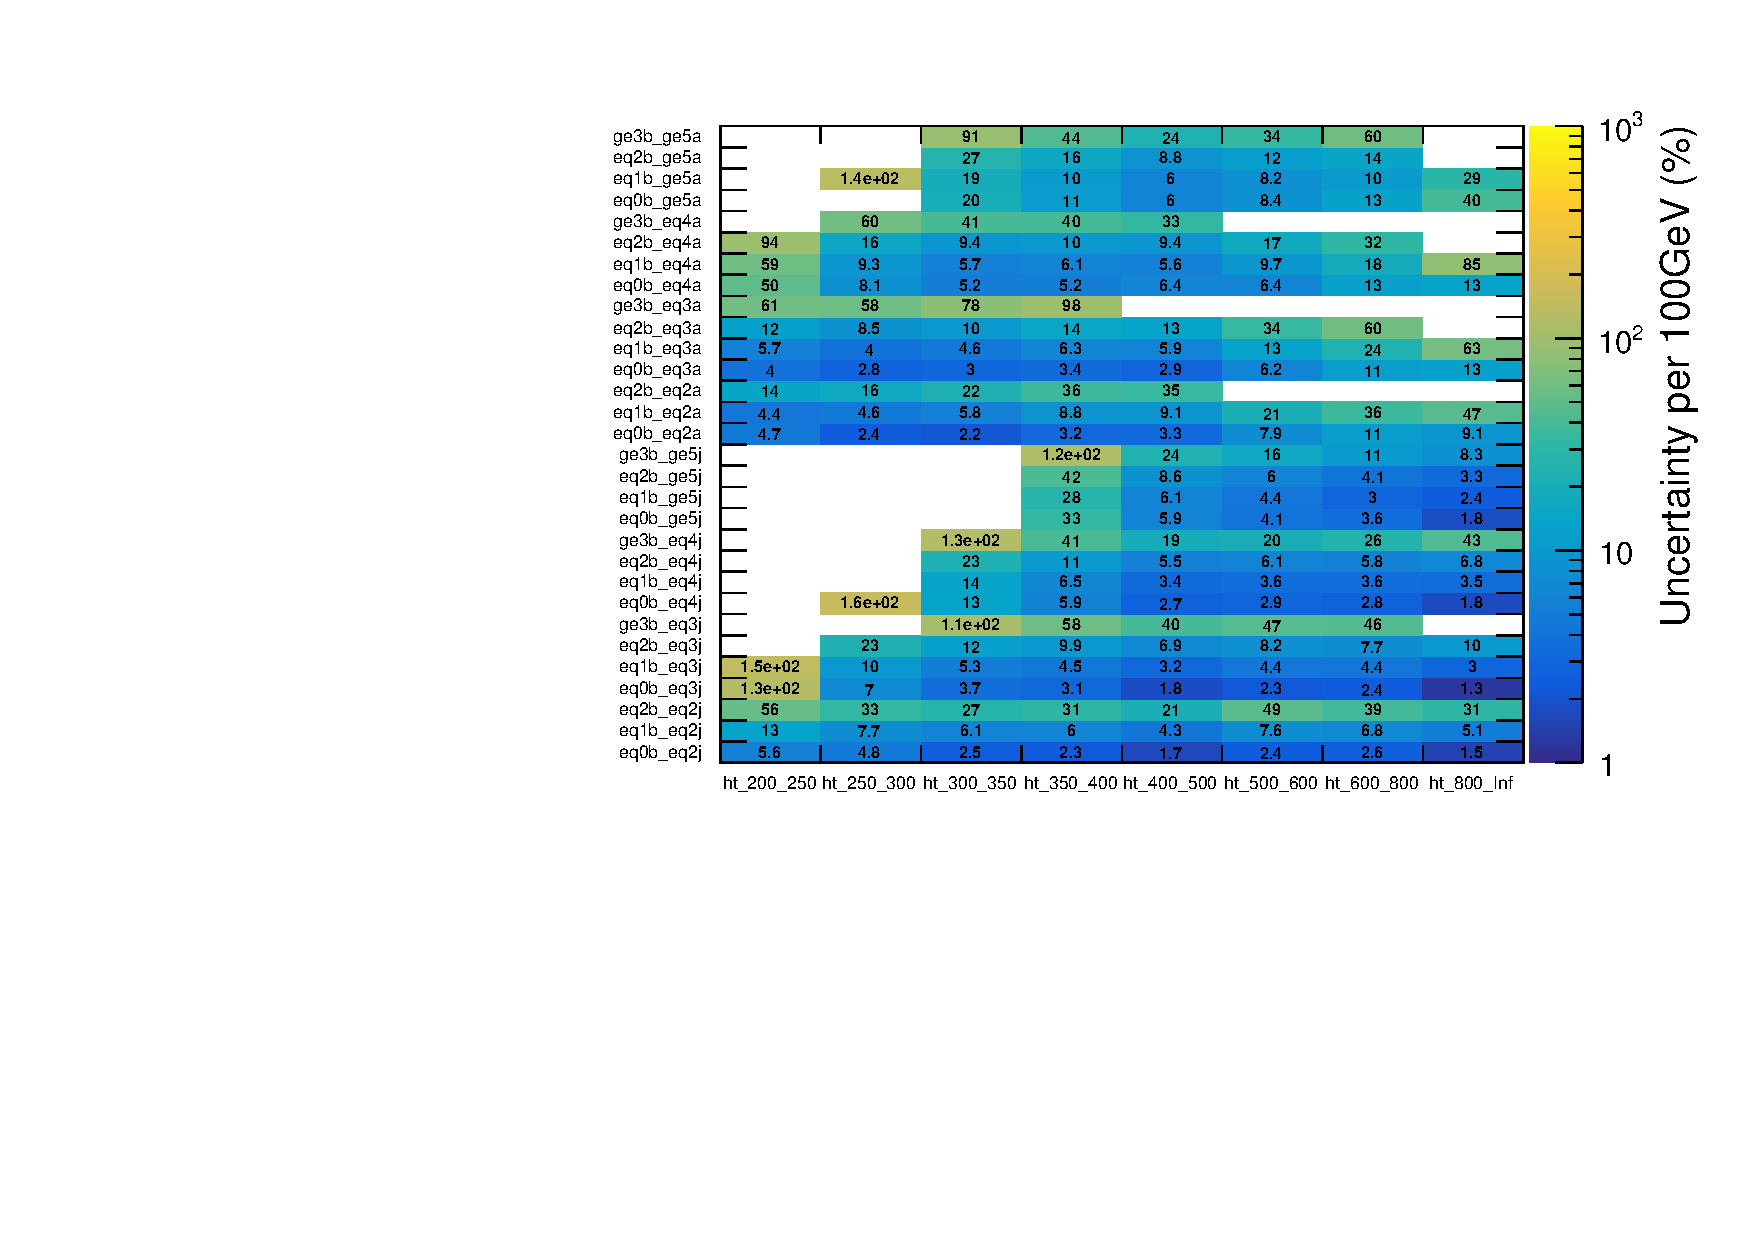
\includegraphics[width=0.5\textwidth]{Figures/backgroundPrediction/shapeOutput12FbMC/scale_ht_variable_mht/Zinv/fitOut/Linear2DShiftMean/frenchFlagErrComplete_Linear2DShiftMean_p1_Zinv.pdf}
  }~~
  \subfigure[\label{fig:observedZinv} Observed uncertainties]{
    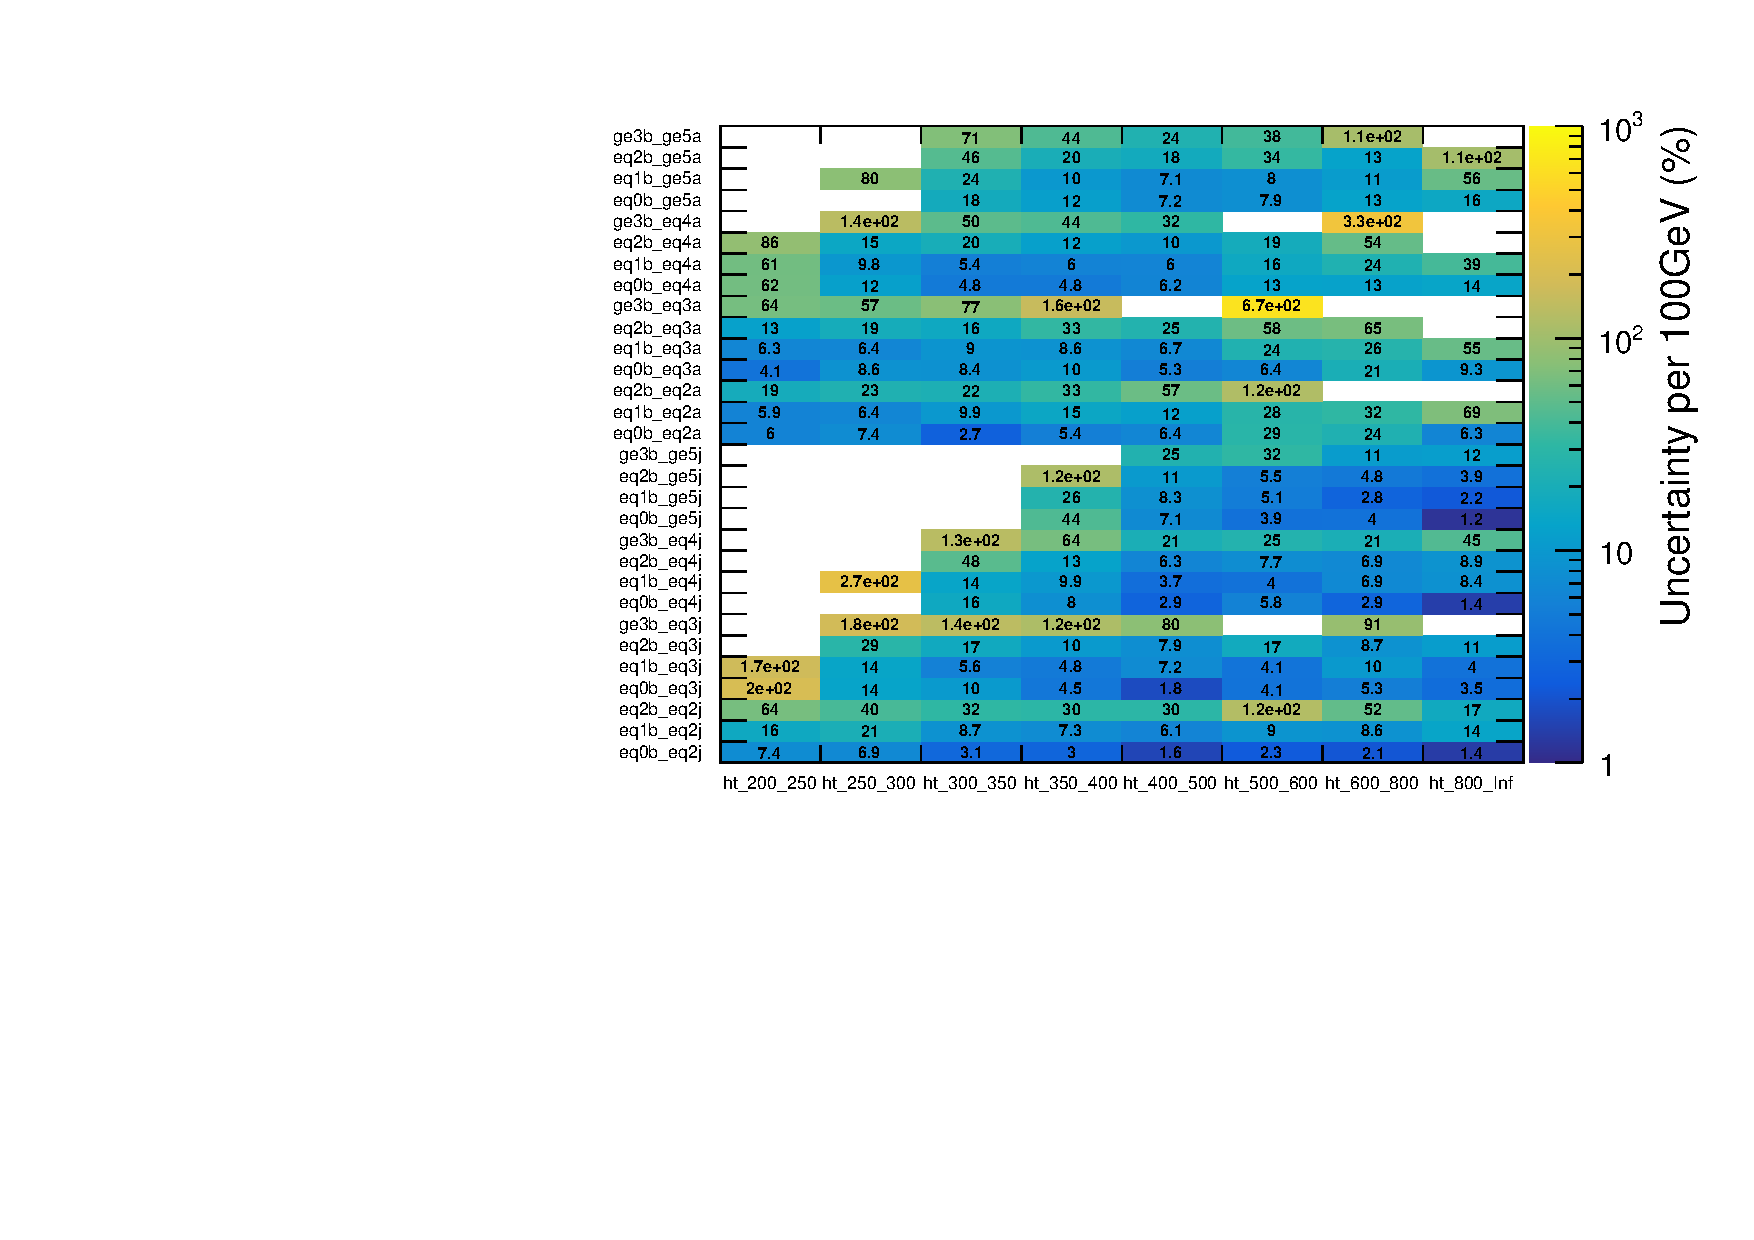
\includegraphics[width=0.5\textwidth]{Figures/backgroundPrediction/shapeOutput12Fb/scale_ht_variable_mht/Zinv/fitOut/Linear2DShiftMean/frenchFlagErrComplete_Linear2DShiftMean_p1_Zinv.pdf}
  }\\
  \caption{\label{fig:expectedObservedZinv}Expected relative uncertainties per 100 \GeV shown for \zInv~ in Fig.~\ref{fig:expectedZinv} are consistent
  with observed uncertainties shown in Fig.~\ref{fig:observedZinv}.}
\end{figure}


% \begin{figure}[h!]
%   \centering
%   \includegraphics[width=0.8\textwidth]{figures/template13TeV/2p2fb/frenchFlagLastBin.pdf}
%   \caption{\label{fig:frenchFlagLastBin} Observed uncertainties in the 
%   last bin of \mht over all categories and \scalht bins for 2.2\ifb.}
% \end{figure}

\newpage
\subsection{Inclusion of systematic sources from simulation}
\label{sec:mcSystStudiesShape}

The size of the variation of the \mht distribution under $\pm1\sigma$ shifts of the
sources of systematic uncertainty described in Section ?? is compared 
to that of the orthogonal polynomial systematic described in \ref{sec:valid13}.
As for the transfer factor variations, for each source of systematic the prediction 
is varied by $\pm1\sigma$. In the likelihood, the \mht shape and transfer factors
are varied simultaneously for each source of uncertainty, as discussed in Section ??.

To study the effect of the systematic variations on the \mht shape (and not normalisation) 
the resulting template is normalised to the nominal template in each jet category and \scalht bin. 
Figures~\ref{fig:mcCompLow} and \ref{fig:mcCompHigh} show the variations for two representative \scalht 
bins and jet-categories. 
% To show the effect across all jet categories, except the monojet categories for which the \mht dimension is not used,
% and \scalht bins Fig~\ref{fig:lastBinVar} shows the maximum upwards/downwards variation in the last 
% \mht bin as a proportion of the orthogonal polynomial variation.

\begin{figure}[h!]
  \centering
  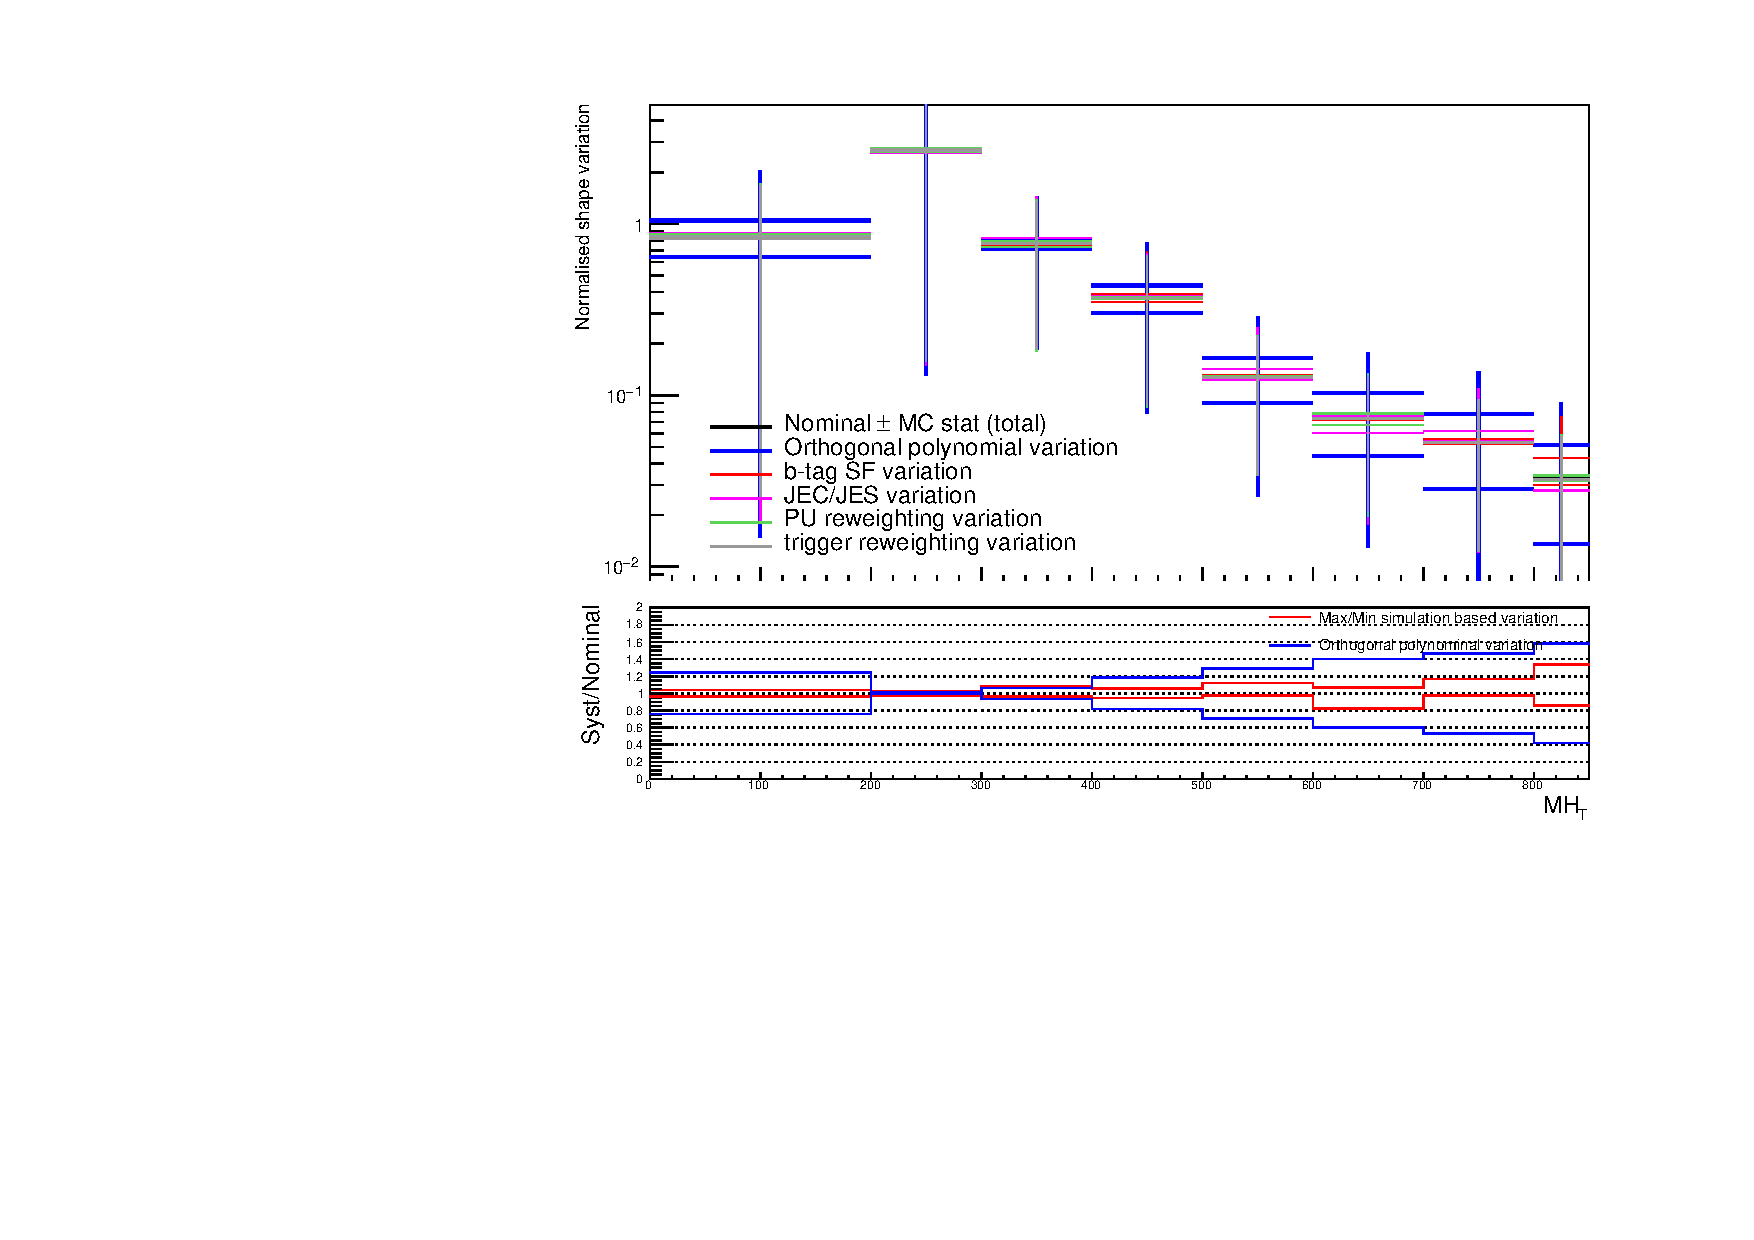
\includegraphics[width=0.8\textwidth]{Figures/backgroundPrediction/mcComparison6fb/totalSMS-T1tttt_mGluino-1000_mLSP-100_25ns_mht_ge5j_ge3b_800.pdf}
  \caption{\label{fig:mcCompLow} MC based systematic variations shown to be considerably smaller 
  than the orthogonal polynomial data-driven systematic for an example bin \scalht $800-\infty$, \njet $\geq 5$, \nb $\geq 2$.}
\end{figure}
\begin{figure}[h!]
  \centering
  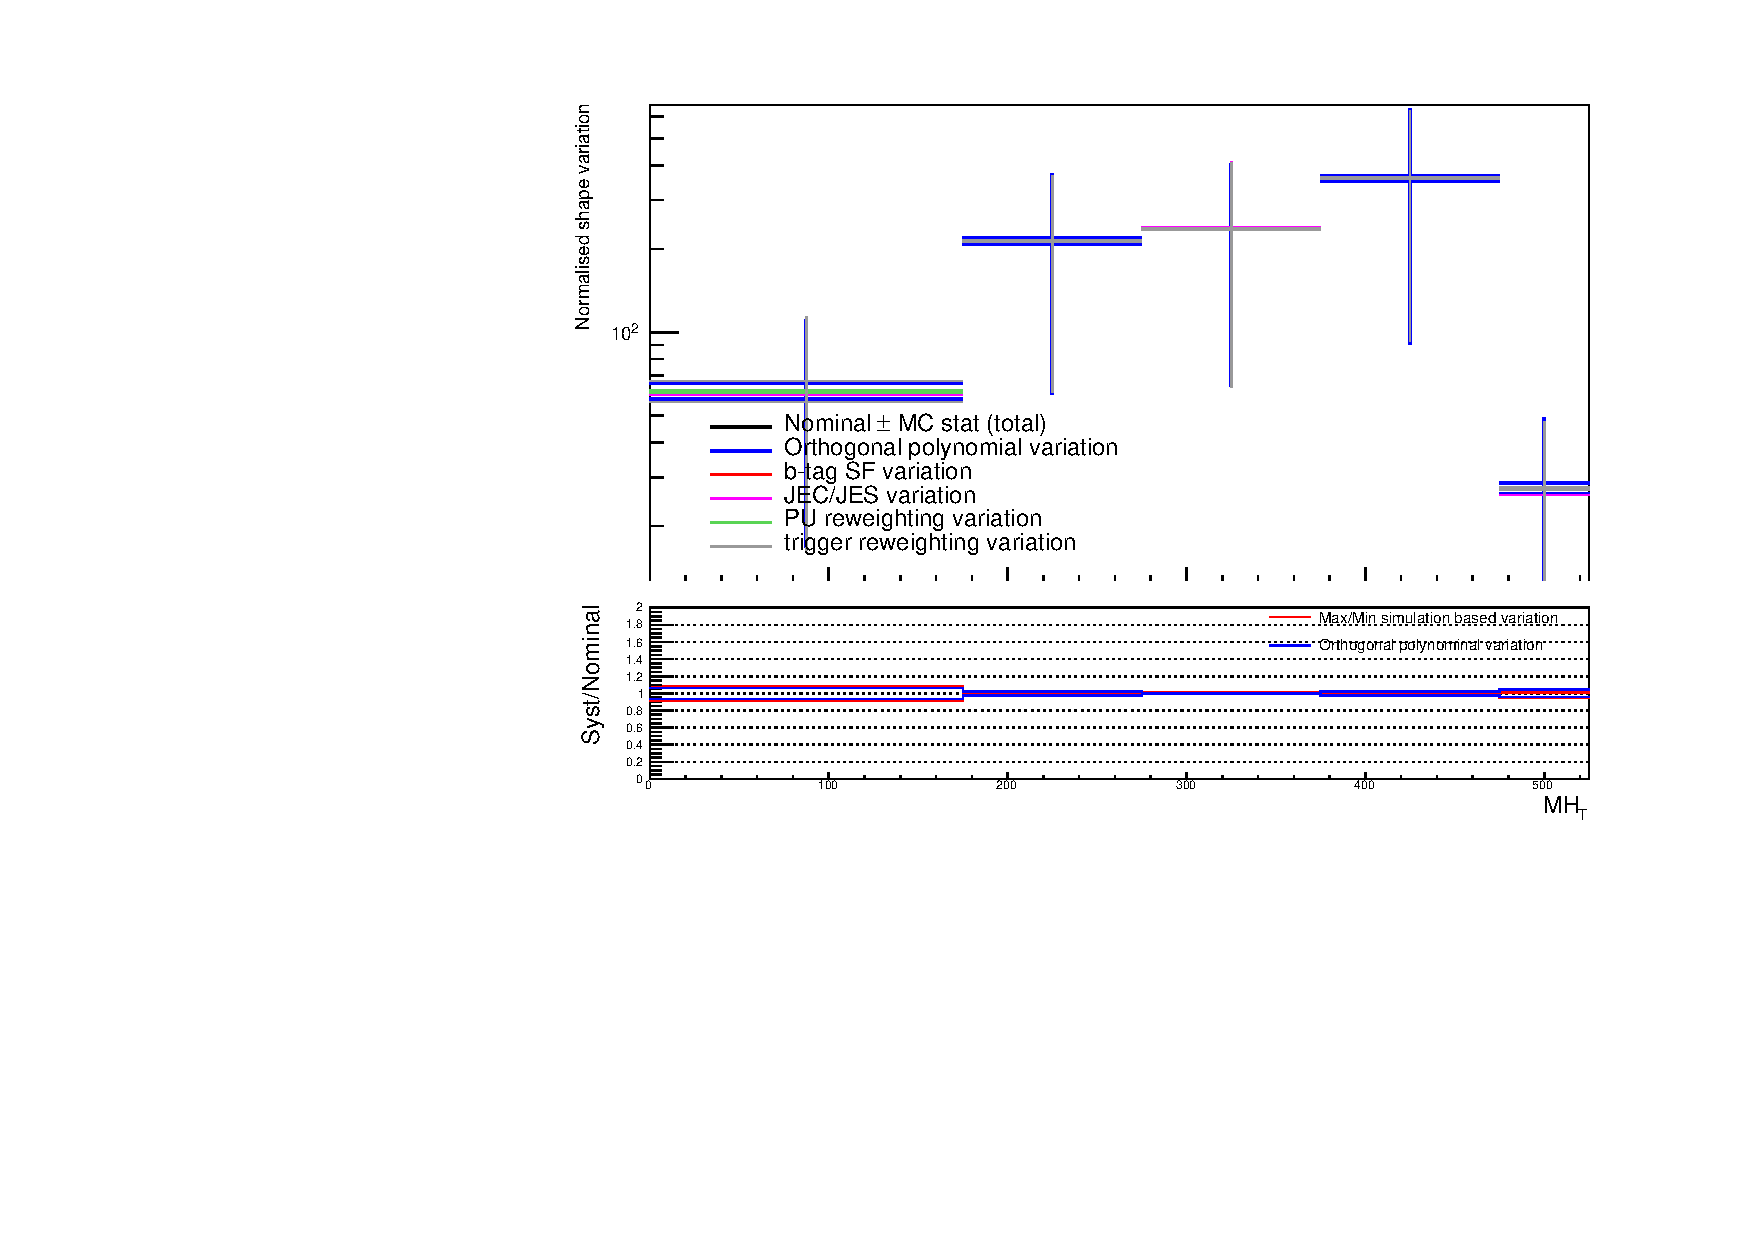
\includegraphics[width=0.8\textwidth]{Figures/backgroundPrediction/mcComparison6fb/totalSMS-T1tttt_mGluino-1000_mLSP-100_25ns_mht_eq2j_eq0b_400.pdf}
  \caption{\label{fig:mcCompHigh} MC based systematic variations shown to be considerably smaller 
  than the orthogonal polynomial data-driven systematic for an example bin \scalht 400-500, \njet $= 2$, \nb $= 0$.}
\end{figure}

% \begin{figure}[h!]
% \centering
% \subfigure[Upwards deviation]{
% \includegraphics[width=0.5\textwidth]{Figures/backgroundPrediction/mcComparison6fb/lastBinRatioMax.pdf}
% }
% \subfigure[Downwards deviation]{
% \includegraphics[width=0.5\textwidth]{Figures/backgroundPrediction/mcComparison6fb/lastBinRatioMin.pdf}
% }\\
% \caption{\label{fig:lastBinVar} Maximum upwards and downwards variations in the last \mht bin as a proportion of the orthogonal polynomial deviation}
% \end{figure}


